%!TEX root = ./ERL Industrial Robots-rulebook.tex

%--------------------------------------------------------------------
%--------------------------------------------------------------------
%--------------------------------------------------------------------

\section{Introduction to \erlir}
\label{sec:Intro}
The objective of the \erl is to organize several indoor robot competition events per year, ensuring a
scientific competition format, around the following two challenges: \erlsr and \erlir.
Those indoor robot competitions will be focused on two major challenges addressed by H2020: societal
challenges (service robots helping and interacting with humans at home, especially the elderly and
those with motor disabilities) and industrial leadership (industrial robots addressing the flexible factories of the future and modern automation issues). These challenges were addressed by \ro and \rockeutwo and will be extended in the \erl by building on the current version of the
rule books and testbeds designed and used during RockEU2’s project lifetime.


Greater automation in broader application domains than today is essential for ensuring European industry remains competitive, production processes are flexible to custom demands and factories can operate safely in harsh or dangerous environments.  
In the \erlir competition, robots will assist with the assembly of a drive axle - a key component of the robot itself and therefore a step towards self-replicating robots. 
Tasks include locating, transporting and assembling necessary parts, checking their quality and preparing them for other machines and workers. 
By combining the versatility of human workers and the accuracy, reliability and robustness of mobile robot assistants, the entire production process is able to be optimized. 

The \erlir competition is looking to make these innovative and flexible manufacturing systems, such as that required by the \rollin factory, a reality. 
This is the inspiration behind the challenge and the following scenario description.
A more detailed account of the \erlir competition, but still targeted towards a general audience, is given in the \erlir in a Nutshell document, which gives a brief introduction to the very idea of the \erl and the \erlir competition, the underlying user story, and surveys the scenario, including the environment for user story, the tasks to be performed, and the robots targeted.
Furthermore, this document gives general descriptions of the task benchmarks and the functional benchmarks that make up \erlir. 
The document on hand is the rule book for \erlir, and it is assumed that the reader has already read the nutshell document. 
The audience for the current document are teams who want to participate in the competition, the organizers of events where the \erlir competition is supposed to be executed, and the developers of simulation software, who want to provide their customers and users with ready-to-use models of the environment. 


The remainder of this document is structured as follows:
Section \ref{sec:AwardCategories}, \emph{\textbf{award categories}} surveys the number and kind of awards that will be awarded and how the ranking of the award categories is determined based on individual benchmark results.
The \emph{\textbf{testbed}} for \erlir competitions is described in some detail in the next section (Section \ref{sec:TestBed}). 
Subsections are devoted to the specification of the structure of the environment and its properties (Section \ref{ssec:StructureProperties}), to the mechanical parts and objects in the environment which can be manipulated (Section \ref {sssec:PartstoManipulate}), to objects in the environment that need to be recognized for completing the task (Section \ref{sssec:EnvironmentObjectstoRecognize}), to the networked devices embedded in the environment and accessible to the robot (Section \ref{ssec:NetworkedDevices}), and to the benchmarking equipment which we plan to install in the environment and which may impose additional constraints to the robot's behavior (equipment presenting obstacles to avoid) or add further perceptual noise (visible equipment, see Section \ref{ssec:BenchmarkingEquipment}).
Next (Section \ref{sec:RobotsTeams}), we provide some specifications and constraints applying to the \emph{\textbf{robots and teams}} permitted to participate in \erlir. 
The \erl consortium is striving to minimize such constraints, but for reasons of safety and practicality such constraints are required. 
After that, the next two sections describe in detail the \emph{\textbf{task benchmarks}} (Section \ref{sec:TaskBenchmarks}) and the \emph{\textbf{functionality benchmarks}} (Section \ref{sec:FunctionalityBenchmarks}) comprising the \erlir competition, while information on scoring and ranking the performance of participating teams on each benchmark is already provided in the benchmark descriptions.%, Section \ref{sec:AwardCategories}, \emph{\textbf{award categories}} surveys the number and kind of awards that will be awarded and how the ranking of the award categories is determined based on individual benchmark results. 
%Last but not least, Section \ref{sec:RoawOrganization} provides details on \emph{\textbf{organizational issues}}, like the committees involved, the media to communicate with teams, qualification and setup procedures, competition schedules, and post-competition activities.   

%--------------------------------------------------------------------
%--------------------------------------------------------------------
%--------------------------------------------------------------------
%!TEX root = ./ERL Industrial Robots.tex

%--------------------------------------------------------------------
%--------------------------------------------------------------------
%--------------------------------------------------------------------
\clearpage\phantomsection
\section{\erlir Award Categories}
\label{sec:AwardCategories}
Awards will be given to the best teams in each of the \erlir \emph{task benchmarks} and \emph{functionality benchmarks} that are described in Sections \ref{sec:TaskBenchmarks} and \ref{sec:FunctionalityBenchmarks}. 
For every local/major tournament, and for every task and functionality benchmark, a score is computed by taking the median of the best (up to 5) trials. The final end of year score is computed by taking the median of the pooled trials that were used for scoring the best two Local/Major tournaments and teams are ranked based on this score.
The \erl Competition awards will be given in the form of cups for the best teams. Every team will also receive a plaquette with the \erl logo and a certificate.

Please note that teams need to participate in a minimum of two tournaments (Local and/or Major) per year in order to obtain a  score for the TBMs and/or FBMs that they intend to enter.

%\erlir competition awards will be given in the form of cups for the best teams, as specified below. Every team will receive a plaquette with the \erlir logo and a certificate.
%Awards will be given to the best teams in \erlir \emph{task benchmarks}, \emph{functional benchmarks} and overall.

%--------------------------------------------------------------------
%--------------------------------------------------------------------
\subsection{Awards for Task Benchmarks}
\label{sec:AwardTBMs}
The team with the highest score in each of the three \emph{task benchmarks} will be awarded a cup (''\erlir Best-in-class Task Benchmark <\emph{task benchmark} title>'').
When a single team participates in a given \emph{task benchmark}, the corresponding \emph{task benchmark} award will only be given to that team if the Executive and Technical Committees consider the team performance of exceptional level. 

%The team with the highest score in each of the three \emph{task benchmarks} will be awarded a cup (''\erlir Best-in-class Task Benchmark <\emph{task benchmark} title>'').
%When a single team participates in a given \emph{task benchmark}, the corresponding \emph{task benchmark} award will only be given to that team if the Executive and Technical Committees consider the team performance of exceptional level.

%--------------------------------------------------------------------
%--------------------------------------------------------------------
\subsection{Awards for Functionality Benchmarks}
\label{sec:AwardFBMs}
The teams with the highest score ranking for each of the three \emph{functionality benchmarks} will be awarded a cup (''\erlir Best-in-Class Functionality Benchmark <\emph{functionality benchmark} title>'' and '\erlir Second-Best-in-Class Functionality Benchmark <\emph{functionality benchmark} title>'').
When less than three teams participate in a given \emph{functionality benchmark}, only the ''\erlir Best-in-class Functionality Benchmark <\emph{functionality benchmark} title>'' award will be given to a team, and only if the Executive and Technical Committees consider that team's performance as excellent.

%The two top teams in the score ranking for each of the three \emph{functionality benchmarks} will be awarded a cup (''\erlir Best-in-class Functionality Benchmark <\emph{functionality benchmark} title>'' and ''\erlir Second-Best-in-class Functionality Benchmark <\emph{functionality benchmark} title>'').

%When less than three teams participate in a given \emph{functionality benchmark}, only the ''\erlir Best-in-class Functionality Benchmark <\emph{functionality benchmark} title>'' award will be given to a team, and this will occur only if the Executive and Technical Committees consider that team's performance as excellent.

%--------------------------------------------------------------------
%--------------------------------------------------------------------
%\subsection{Competition Winners}
%\label{sec:AwardOverall}

%Teams participating in \erlir competitions will be ranked taking into account their overall rank in all the \emph{task benchmarks}.
%\todo{LaberLaberLaber entfernen}
%The overall ranking will be obtained by combining task benchmark rankings using the Social Welfare principle (see \url{http://en.wikipedia.org/wiki/Social_welfare_function}); the overall winning team of \roaw Competition 2015 will be the top team in this combined ranking, and will receive the corresponding award cup (''Best Team \roaw Competition 2015''). The second and third placed teams in the ranking will also receive award cups (respectively ''2nd place \roaw Competition 2015'' and ''3rd place \roaw Competition 2015'')).
%The three awards will be given only if more than 5 teams participate in the competition. Otherwise, only the best team will be awarded, except if it is the single team participating, in which case the Executive and Technical Committees must consider that team performance of exceptional level so as for the team to be awarded. Only teams performing the total of the three tasks will be considered for the ''Best Team \roaw Competition 2015'' award.



%--------------------------------------------------------------------
% EOF
%--------------------------------------------------------------------


%--------------------------------------------------------------------
%--------------------------------------------------------------------
%--------------------------------------------------------------------
\clearpage\phantomsection
\section{The \erlir Testbed}
\label{sec:TestBed}

The testbed for the \erlir competition consists of the arena (e.g. walls, workstation), networked devices and task-related objects. The robot can communicate and interact with the networked devices, which allow the robot to exert control on the testbed to a certain extend. 
Figure \ref{fig:rockin-n-rollin-production-area} shows the evolution of the \erlir environment from its early concept in \roaw to its implementation in the \roaw event in Lisbon in 2015 and \roaw last event in Polimi in 2017.
Participating teams should assume the competition environment to be similar to those shown in Figure \ref{fig:rockin-n-rollin-production-area}; deviations should only occur if on-site constraints (space available, safety regulations) enforce them.
%
\begin{figure}[htb]
  \begin{center}
  	\hfill
	  \subfigure[Early concept]{
		  \scalebox{1.0}[1.0]{
  		  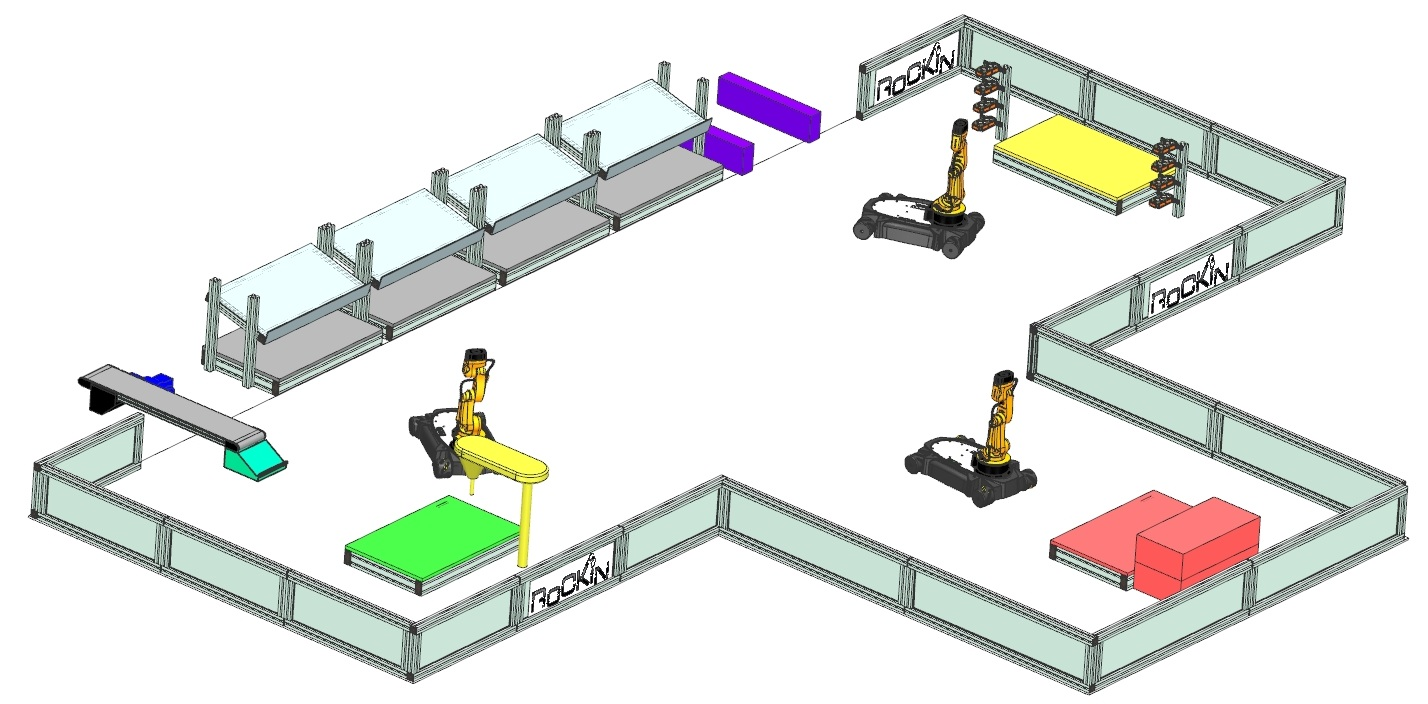
\includegraphics[height=40mm,angle=0,trim=0px 0px 0px 0px,clip]
	  		{fig/AS_RoaW_Arena_v4}
			}
		  \label{fig:RulebookArenaConcept}
		}%
		\hfill
	  \subfigure[Laboratory installation]{
		  \scalebox{1.0}[1.0]{
  		  \includegraphics[height=40mm,angle=0,trim=0px 100px 0px 200px,clip]%
	  		{pics/atwork/test_beds/WorkArenaBRSU.jpg}%
			}
		   \label{fig:RulebookArenaLab}
		}%
		\hfill
		 \subfigure[RoCKIn@Work 2015]{
		  \scalebox{.5}[.5]{%
  		  \includegraphics[height=80mm,angle=0,trim=-200px 0px -250px 0px,clip]%
	  		{fig/testbed/roaw_arena_lisbon.JPG}%
			}%
			\label{fig:RulebookArena2014}
		}%
		\hfill
		\subfigure[RoCKIn@Work 2017]{
			\scalebox{.5}[.5]{%
				\includegraphics[height=80mm,angle=0]%
				{fig/testbed/roaw_arena_polimi.jpg}%
			}%
			\label{fig:RulebookArenaLisbon2015}
		}%
		\hfill\mbox{}
	  \caption{The evolution of the \erlir environment}
  	\label{fig:rockin-n-rollin-production-area}
	\end{center}
\end{figure}

%!TEX root = ./ERL Industrial Robots-rulebook.tex

%--------------------------------------------------------------------
%--------------------------------------------------------------------
\subsection{Environment Structure and Properties}
\label{ssec:StructureProperties}

\noindent
The following set of scenario specifications must be met by the \erlir environment.
%-----------
\begin{envSpec}[Structured Environment]
The environment can consists of various numbers of spatial areas:
	\begin{enumerate}
	\renewcommand{\itemsep}{0.1ex}
	\item rows of shelves
	\item rows of workstations
	\end{enumerate}
	Figure \ref{fig:ArenaArea} shows an example of these areas in the \erlir environment.
The spatial areas extend beyond the space occupied by the respective workstations or objects and include the surrounding area as well. 
\end{envSpec}

%-----------
\begin{envSpec}[Flat Environment]
	All spatial areas are located on the same level, except where 
	specified otherwise. There are no stairs in the environment.
\end{envSpec}

%-----------
\begin{envSpec}[Spatial Areas and Rooms]
The factory is a single, large open space; there are no rooms separated by walls in the environment. 
Spatial areas can be partially separated by dividing or protective walls or other objects present in the factory (e.g. shelves, workstations, platforms, tables).
\end{envSpec}

%-----------

\begin{figure}[!htbp]
  \begin{center}
  	  \scalebox{1.0}[1.0]{%
  		  \includegraphics[width=140mm,angle=0, trim=0px 0px 0px 0px,clip]%
	  		{./fig/WorkArenaBRSUSpatialArea.jpg}%
			}%
	   	\caption{Example of the spatial areas in the \erlir environment. The spatial areas are shelves (red), force fitting workstation (blue), conveyor belt (green), drilling workstation (orange) and assembly workstation (yellow).}
  	\label{fig:ArenaArea} 
  \end{center}
\end{figure}

%-----------
\begin{envSpec}[Dimensions]
	\label{scenspec:dimensions}
	The precise dimensions and the arrangement of the spatial areas are not predefined, but estimated sizes are given. 
	The estimated sizes of the spatial areas are as follows: workstations $2m\times2m $ and shelves $5m\times0,5m$.
	The bounding box of the environment has a minimum area of $16 m^2$ and a maximum area of $100 m^2$. More space is used, when areas and workstations are doubled for teams working in parallel.
\end{envSpec}

%-----------
\begin{envSpec}[Set of Shelves]
The shelves-area is a set of connected shelves and each shelves has two level (upper level and lower level).
The robot can take and/or deliver objects from the shelves (through the containers or directly onto shelves).
Figure \ref{fig:ArenaArea} shows an example of the shelves-area made from two set of shelves.
\end{envSpec}

%-----------
%\begin{envSpec}[Force Fitting Workstation]
%Force fitting workstation has a table for temporarily storing handled parts. 
%The table is part of the force fitting machine which is operated by a robot or human worker. 
%On one side is the assembly aid tray rack to attach filled or unfilled aid trays.
%\end{envSpec}

%-----------
%\begin{envSpec}[Drilling Workstation]
%Drilling workstation consists of a storing area to store ``file card'' boxes and the drilling machine. 
%\end{envSpec}

%-----------
%\begin{envSpec}[Conveyor Belt]
%	The conveyor belt transports parts from outside of the arena into the area.
%	%At the end of the conveyor belt, parts fall down on an exit ramp in a predefined position through guiders where they can be taken by the robot.
%\end{envSpec}

%-----------
\begin{envSpec}[Workstations]
Workstations are used as storage areas for objects. They may be accessible from different locations, i.e. it might be possible to reach a workstation from two or more sides. Additional, there are workstations of different heights present in the environment, ranging from 0 cm up to 15 cm. If a workstation has a height of 0 cm, a tape will mark the area (see Figure \ref{fig:barrier_tape_0cm}). The tape will be taped on the floor and is blue/white striped. This tape may be crossed by the robot and does not count as a collision.
\end{envSpec}

\begin{figure} [h!]
	\begin{center}
		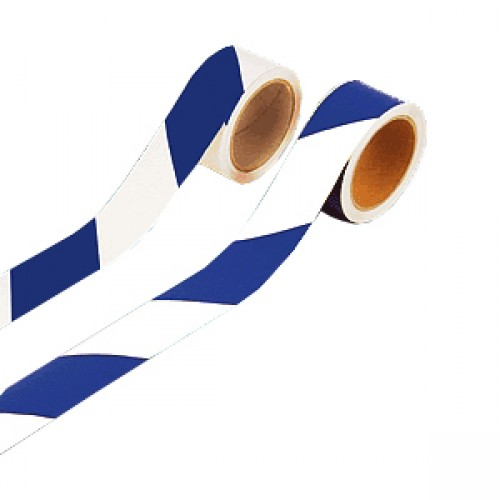
\includegraphics[height = 2.5cm]{pics/atwork/barrier_tape/barrier_tape_0cm_area.jpg}
	\end{center}
	\caption{Barrier tape used to mark workstations with 0 cm height.}
	\label{fig:barrier_tape_0cm}
\end{figure}

%-----------
%\begin{envSpec}[Rotating Table]
%	The rotating table can, similar to a usual workstation, store any kind of object. But compared to a workstation the rotating table is not static and rotating at a constant speed.
%
%\end{envSpec}
	
\begin{envSpec}[Barrier Tape as Virtual Walls]
The environment may include virtual walls marked by either striped yellow/black or white/red barrier tape on the floor (see Figure \ref{fig:barrier_tape}). If any part of a robot passes over such a tape it is considered as a collision with a obstacle. The red/white tape is used to frame the entrance and exit area. The robot is allowed to cross this kind of barrier only at the beginning of a test to enter arena and at the end for leaving. In contrast, the yellow/black one denotes an obstacle which the robot is never allowed to cross.
\end{envSpec}

\begin{figure} [h!]
	\centering
	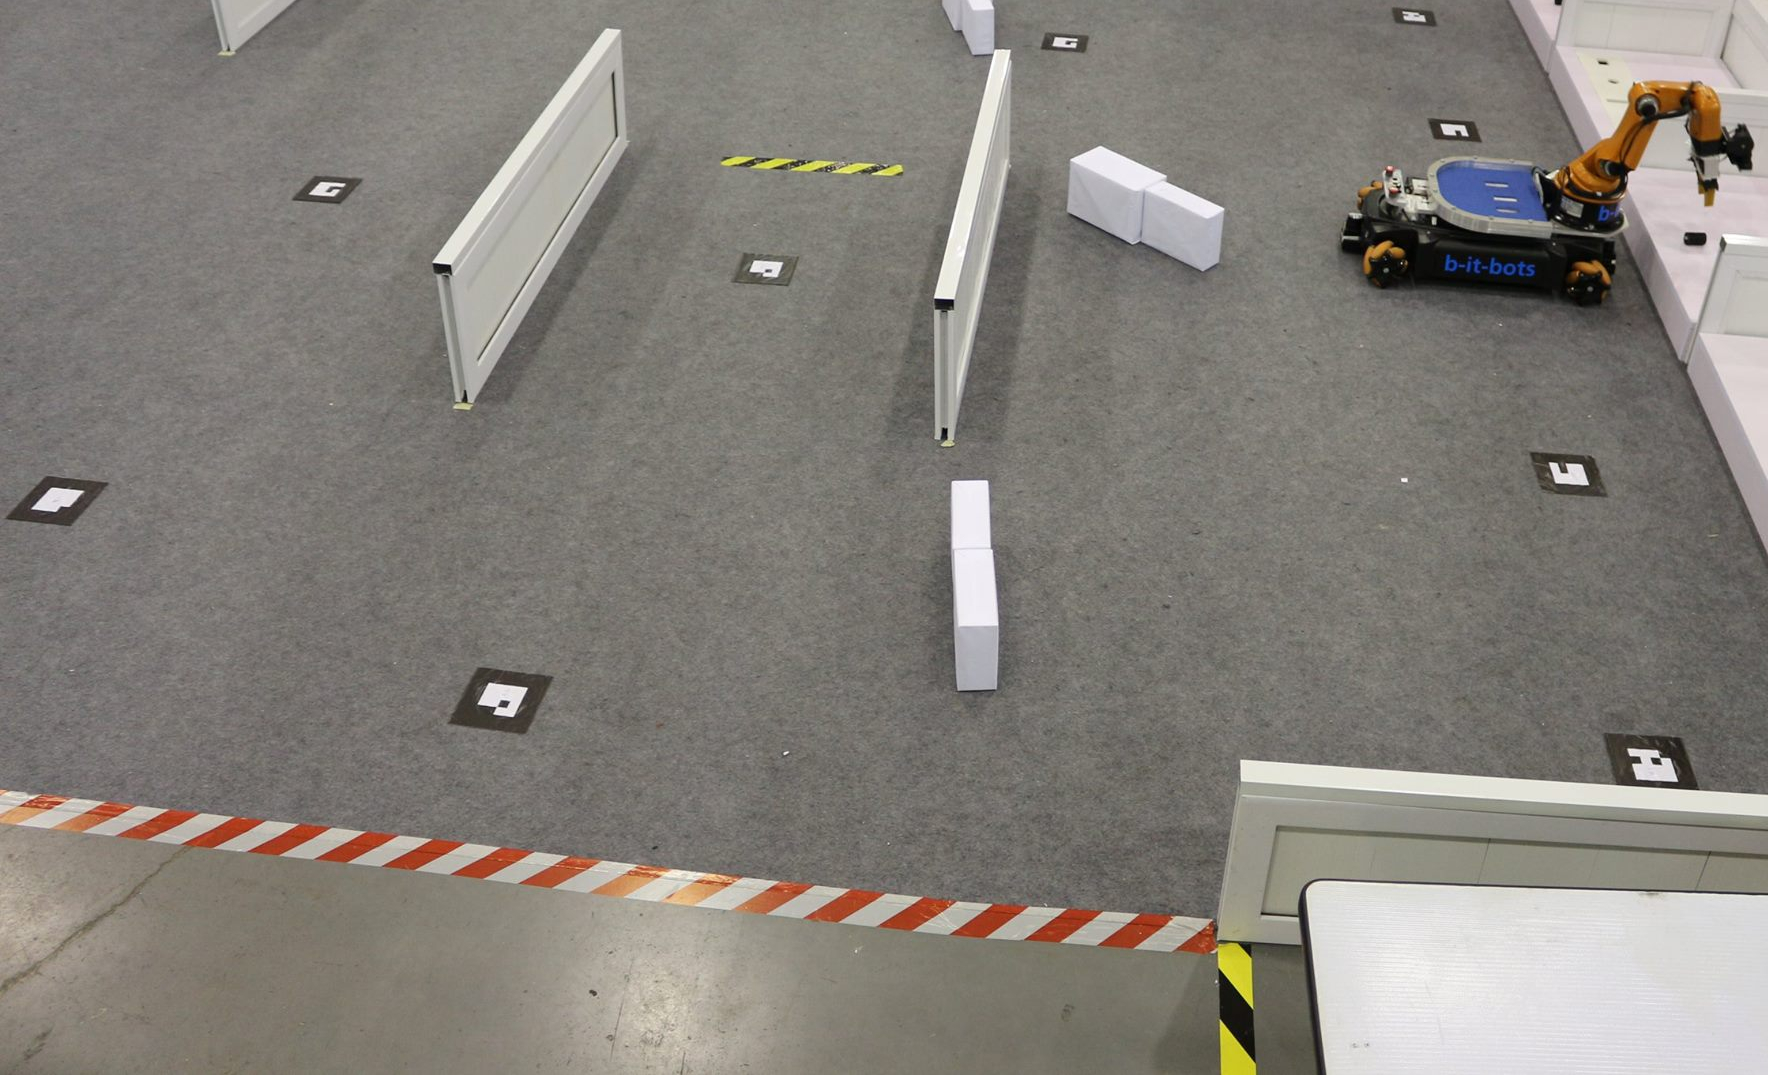
\includegraphics[width= 0.7\textwidth ]{pics/atwork/barrier_tape/barrier_tapes_in_china15.jpg}
	\caption{Example of the different kind of barrier tapes. The red/white tape is used for the entrance and exit, while the yellow/black one denotes an obstacle.}
	\label{fig:barrier_tape}
\end{figure}

%
%
%--------------------------------------------------------------------
% EOF
%--------------------------------------------------------------------

%!TEX root = ./ERL Industrial Robots.tex


%--------------------------------------------------------------------
%--------------------------------------------------------------------
\subsection{Objects in the Environment}
\label{ssec:Objects}

The objects to be manipulated will be selected by the organizer for each tournament.
The following lists describe the different categories of objects that can be used by
the organizer to use during a tournament depending upon the scenario being choosen.
The different categories of objects are:
%
\begin{itemize}
\item Robocup objects 
\item T-LESS dataset objects
\item Chocolate objects
\end{itemize} 
%
%These objects are listed in Table \ref{tab:DriveAxlePartsRulebook} and \ref{tab:ObjectsToRecognize}.

%--------------------------------------------------------------------
\subsubsection{Manipulation Objects}
\label{sssec:PartstoManipulate}
\newcommand*{\ObjectTablePartsImageScale}{0.12\textwidth}

\begin{figure}[hht]
\centering
\subfigure[Bearing Box]{

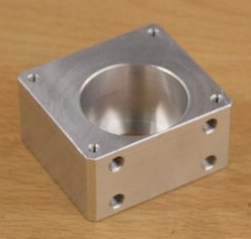
\includegraphics[width=\ObjectTablePartsImageScale, trim=0px 0px 0px -20px, clip] {pics/atwork/objects/bearingBoxA.jpg}
   \label{fig:subfig1}
}
\subfigure[Motor]{
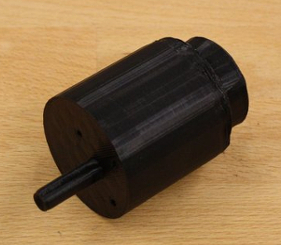
\includegraphics[width=\ObjectTablePartsImageScale, trim=0px 0px 0px -20px, clip] {pics/atwork/objects/motor.jpg} 
   \label{fig:subfig2}
}
\subfigure[Axis]{
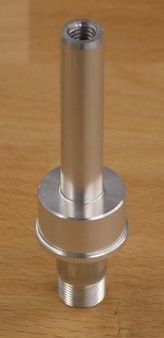
\includegraphics[width=\ObjectTablePartsImageScale, trim=0px 0px 0px -20px, clip] {pics/atwork/objects/axis.jpg} 	
   \label{fig:subfig3}
}
\subfigure[Bearing]{
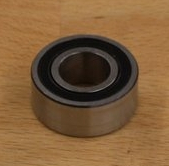
\includegraphics[width=\ObjectTablePartsImageScale, trim=0px 0px 0px -20px, clip] {pics/atwork/objects/bearing.jpg}%		& \texttt{Bearing} 	    		\\  \hline   
   \label{fig:subfig4}
}

\subfigure[F20\_20\_B]{
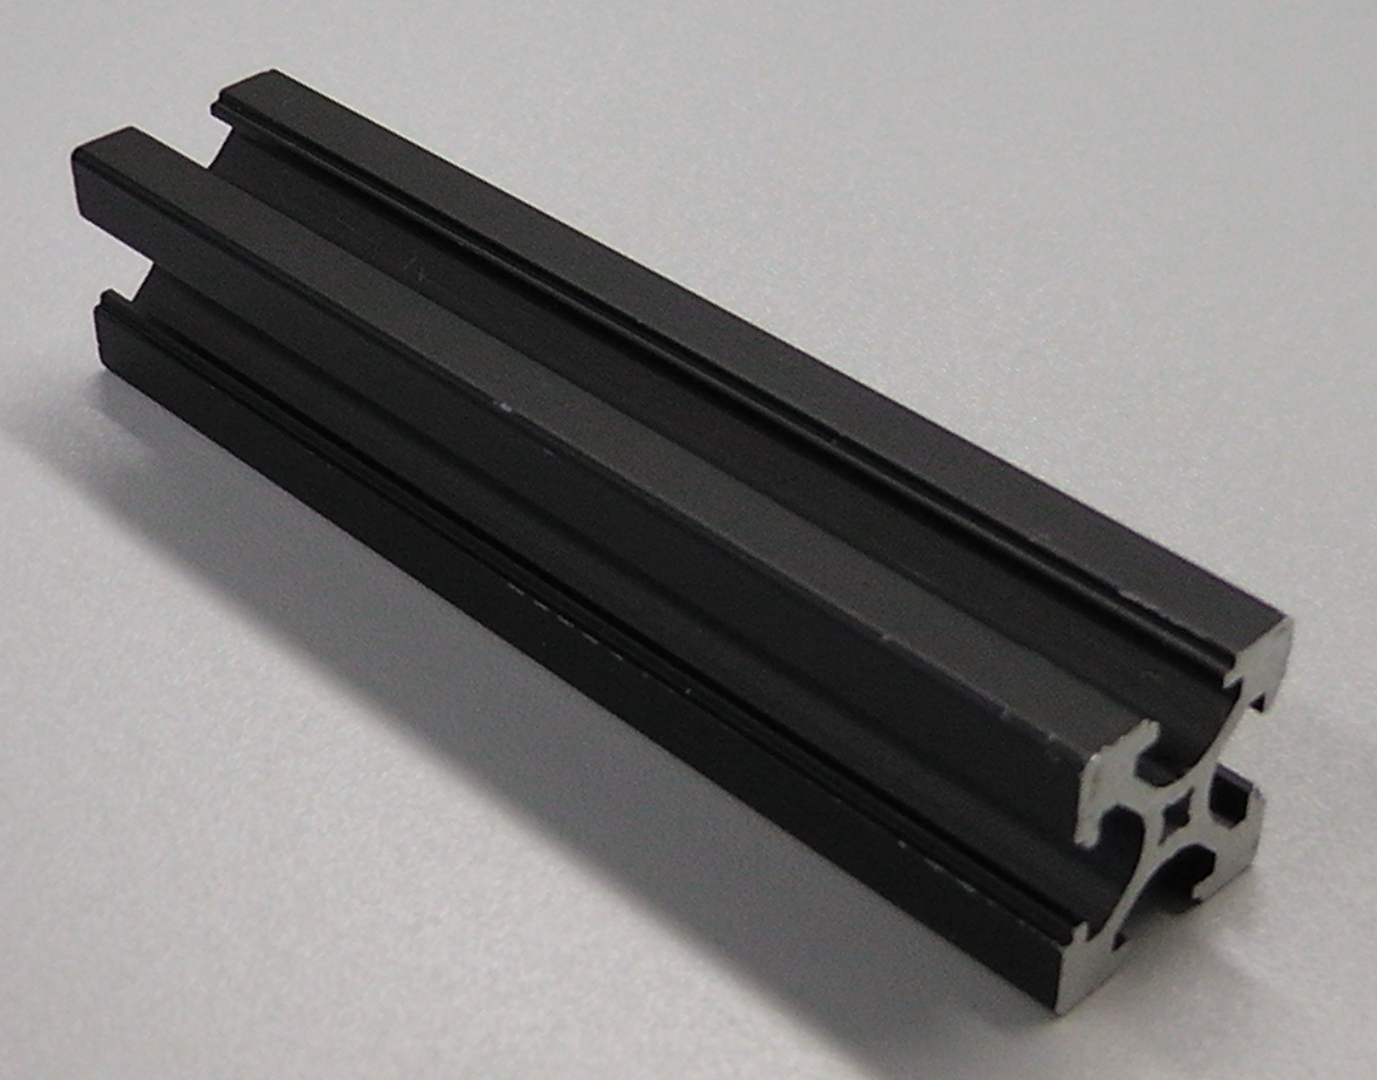
\includegraphics[width=\ObjectTablePartsImageScale, trim=0px 0px 0px -20px, clip] {pics/atwork/objects/F20_20_B.jpg} %	& \texttt{F20\_20\_B}			\\  \hline 
   \label{fig:subfig6}
}
\subfigure[F20\_20\_G]{
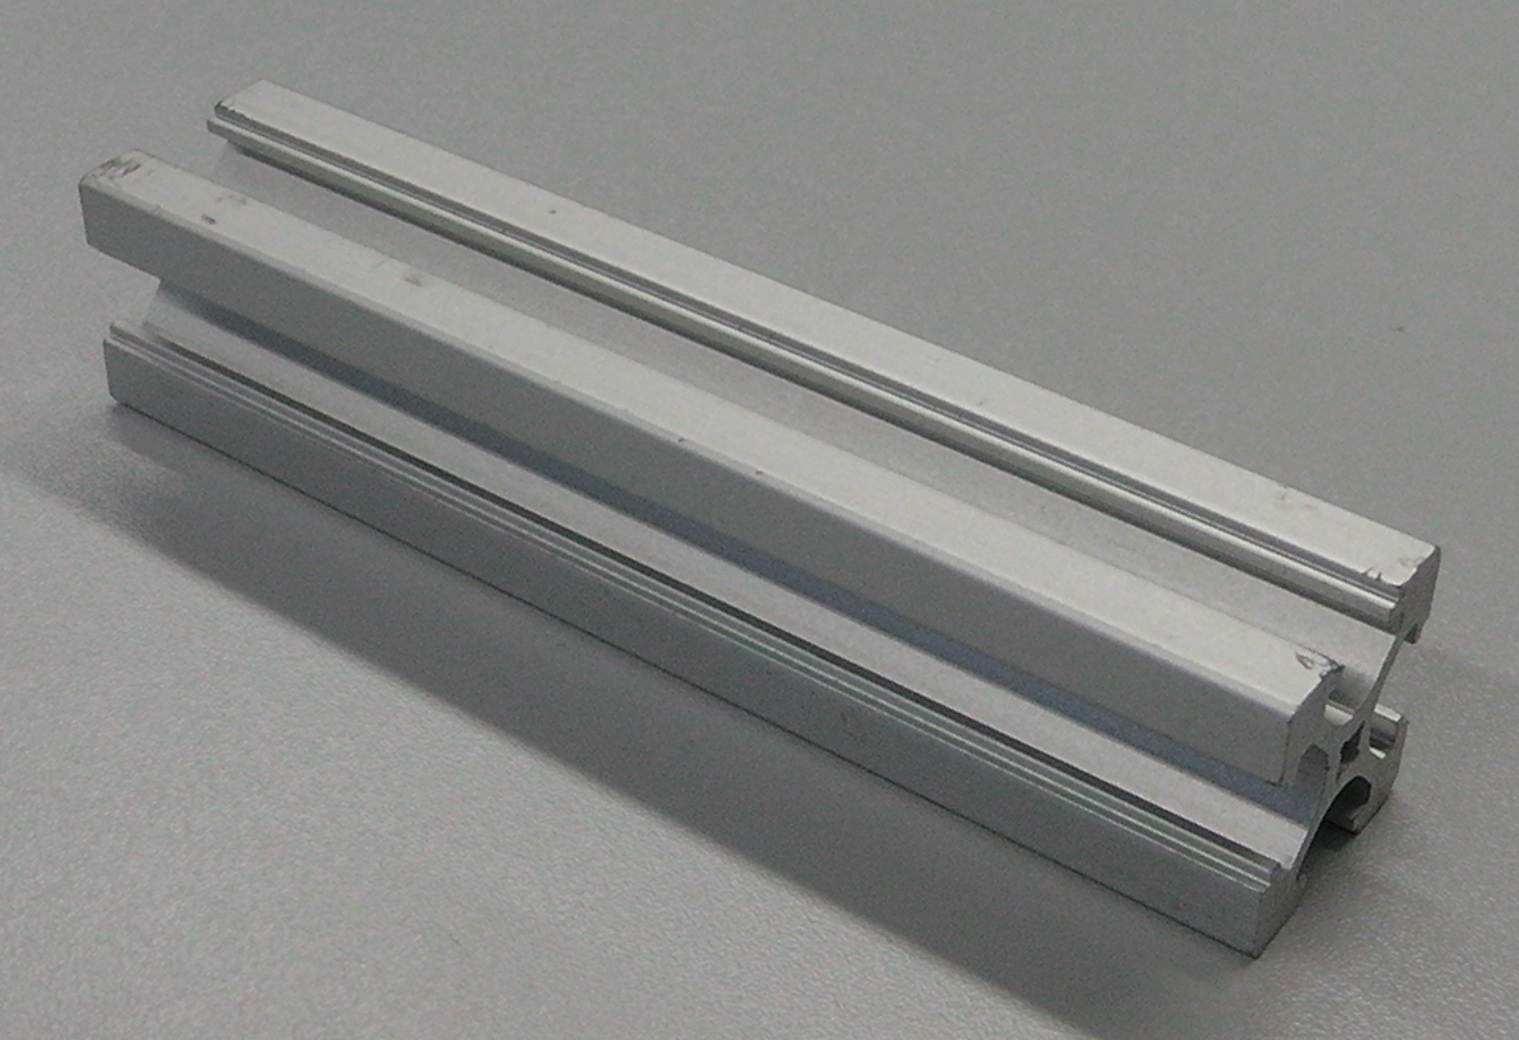
\includegraphics[width=\ObjectTablePartsImageScale, trim=0px 0px 0px -20px, clip] {pics/atwork/objects/F20_20_G.jpg} %	& \texttt{F20\_20\_G}			\\  \hline 
   \label{fig:subfig7}
}
\subfigure[S40\_40\_B]{
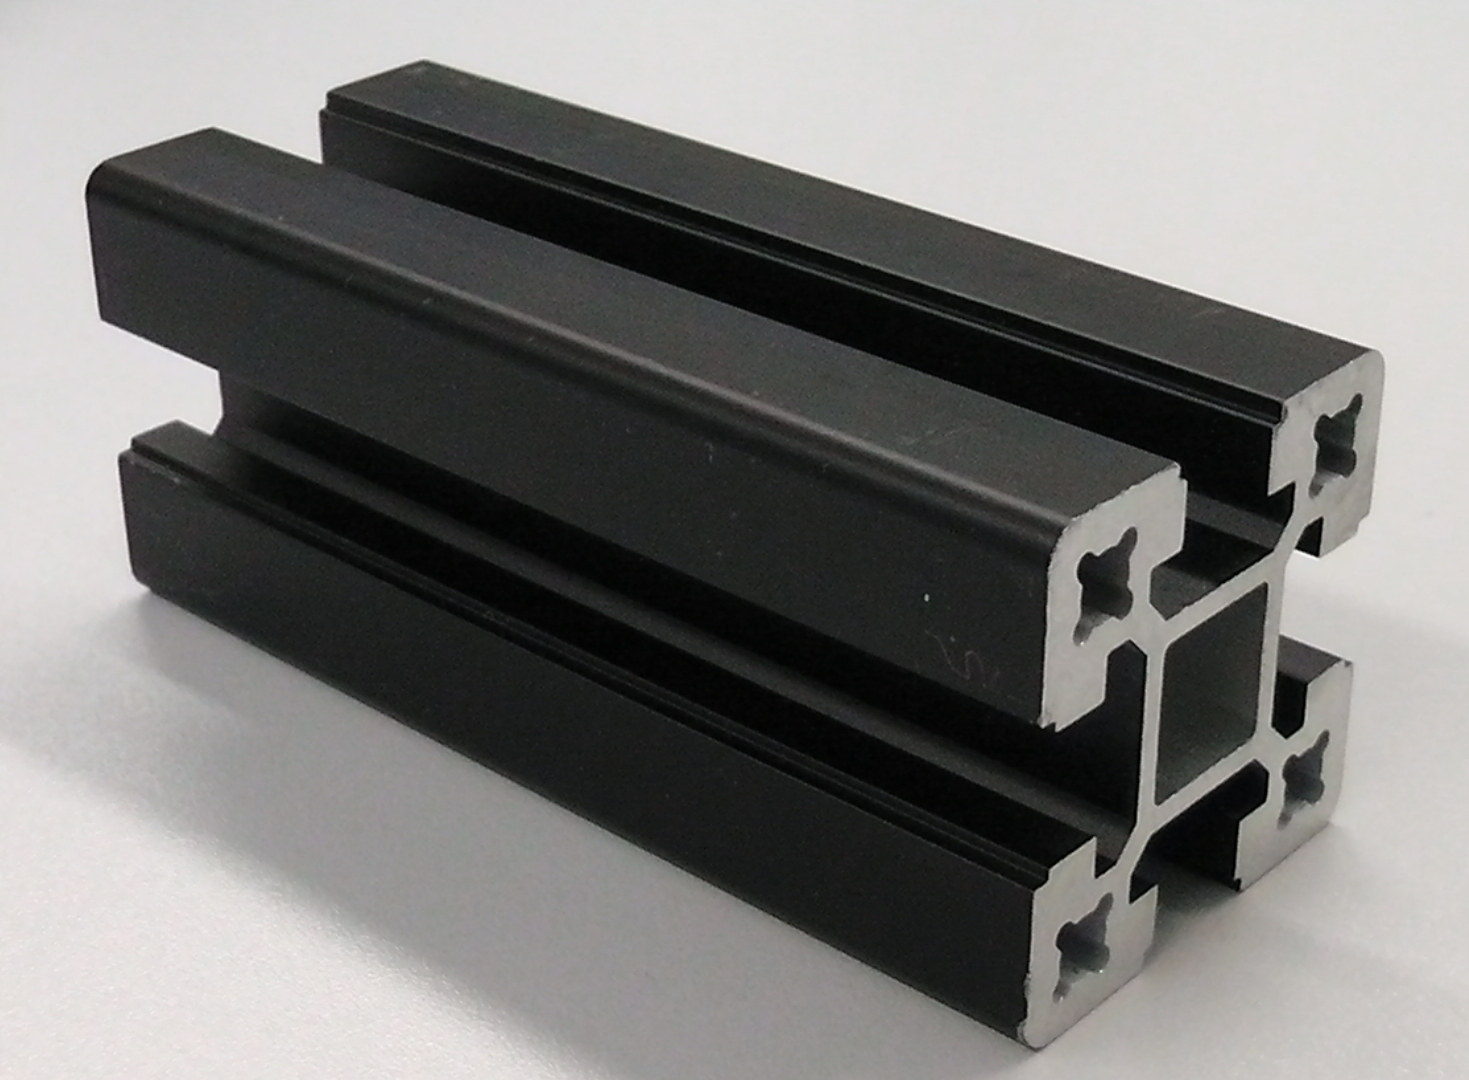
\includegraphics[width=\ObjectTablePartsImageScale, trim=0px 0px 0px -20px, clip] {pics/atwork/objects/S40_40_B.jpg} %	& \texttt{S40\_40\_B}			\\  \hline 
   \label{fig:subfig8}
}
\subfigure[S40\_40\_G]{
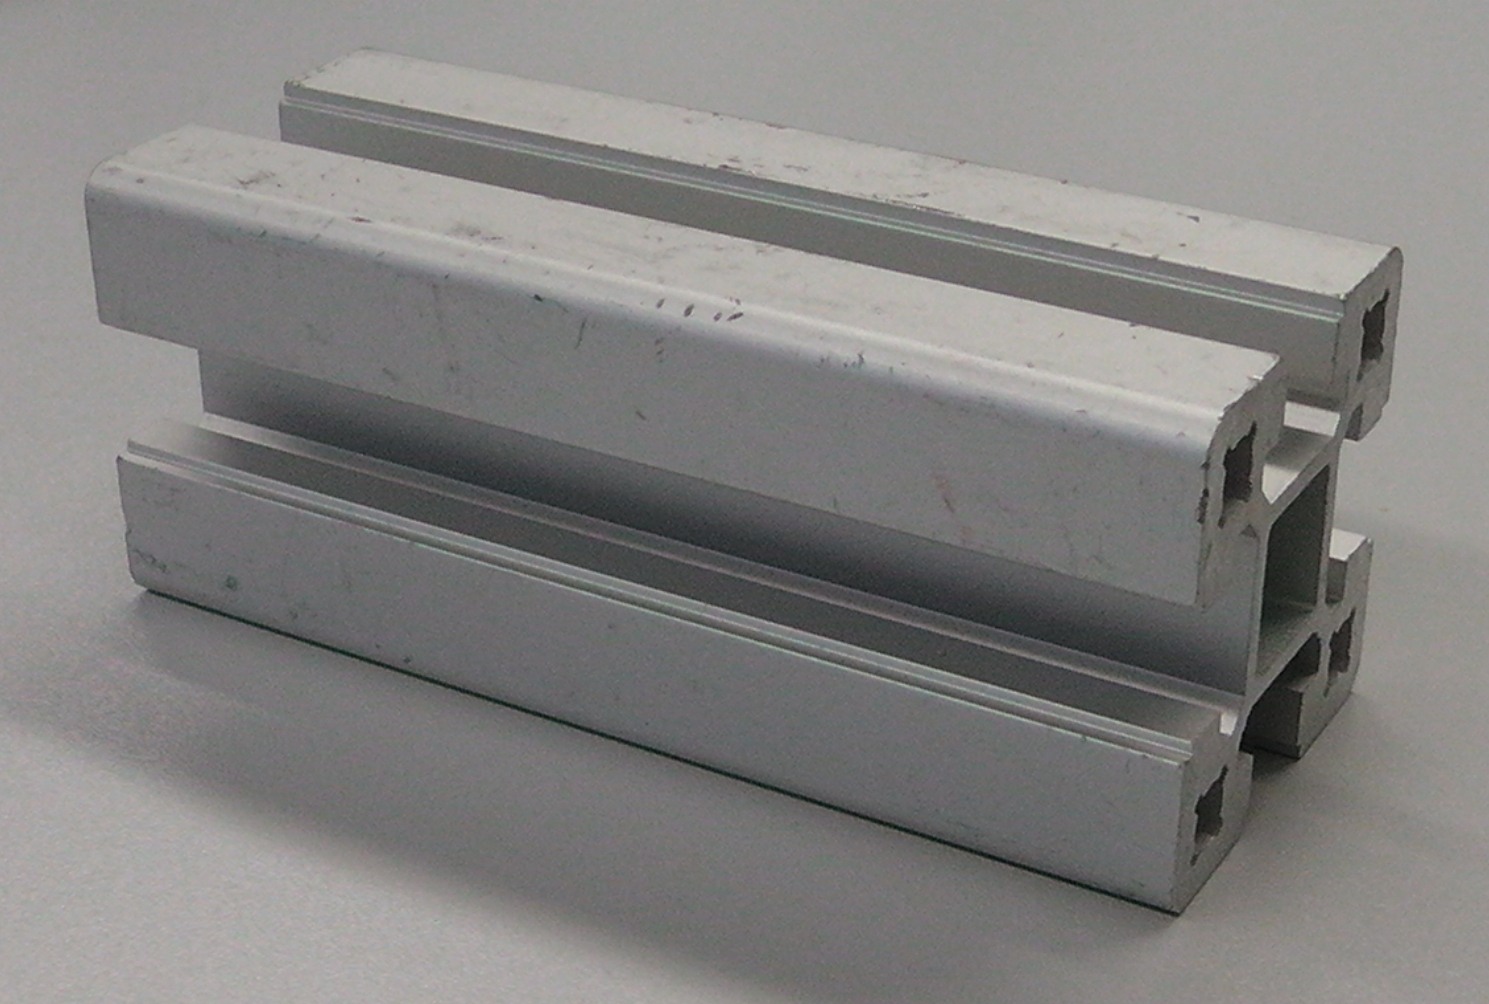
\includegraphics[width=\ObjectTablePartsImageScale, trim=0px 0px 0px -20px, clip] {pics/atwork/objects/S40_40_G.jpg} %	& \texttt{S40\_40\_G}			\\  \hline 
   \label{fig:subfig9}
}
\subfigure[M20\_100]{
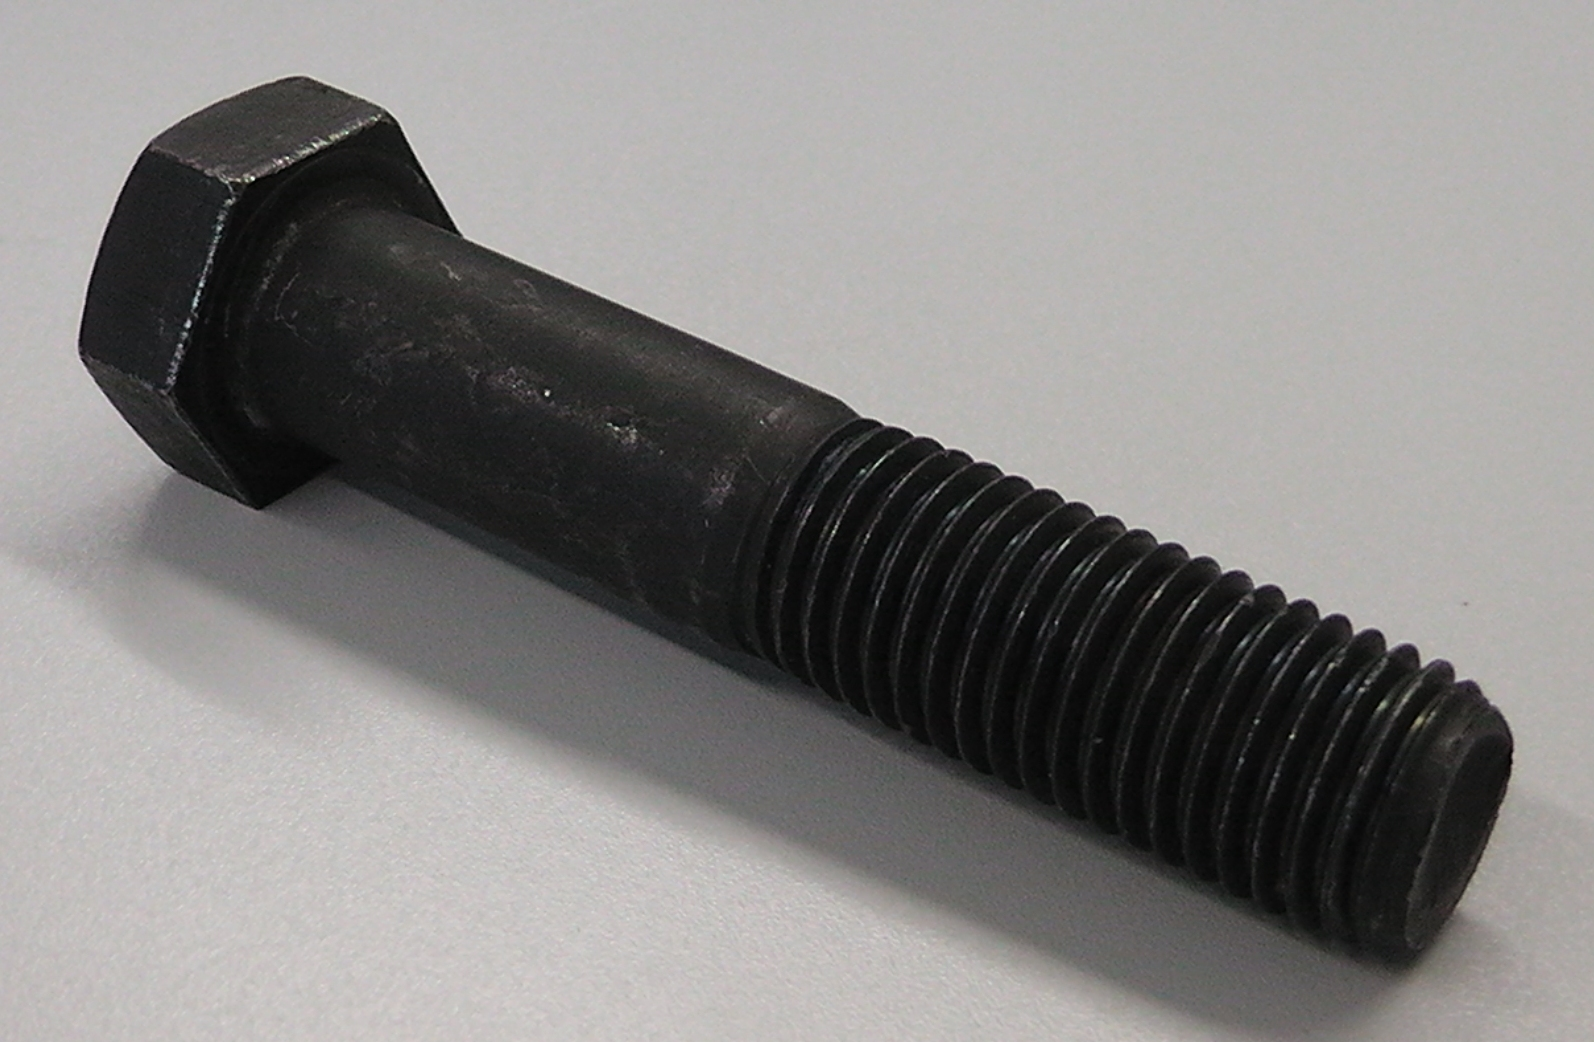
\includegraphics[width=\ObjectTablePartsImageScale, trim=0px 0px 0px -20px, clip] {pics/atwork/objects/M20_100.jpg} 	%	& \texttt{M20\_100}				\\  \hline 
   \label{fig:subfig10}
}
\subfigure[M20]{
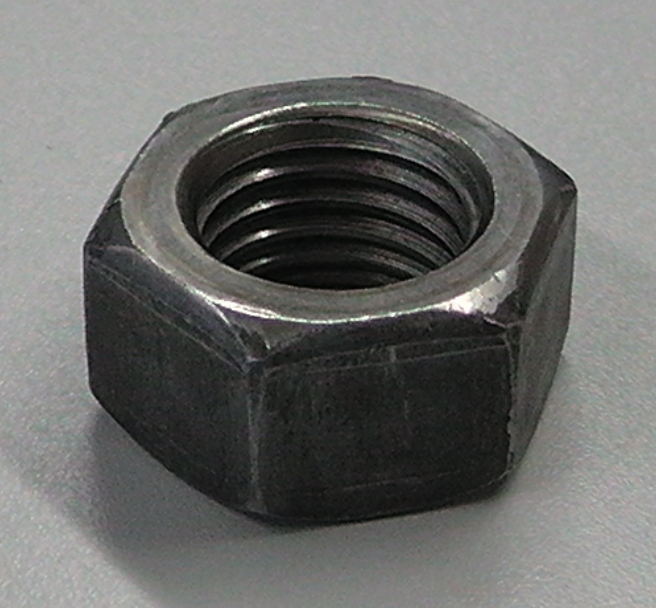
\includegraphics[width=\ObjectTablePartsImageScale, trim=0px 0px 0px -20px, clip] {pics/atwork/objects/M20.jpg} 	%		& \texttt{M20}					\\  \hline 
   \label{fig:subfig11}
}
\subfigure[Distance\_Tube]{
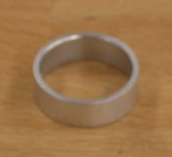
\includegraphics[width=\ObjectTablePartsImageScale, trim=0px 0px 0px -20px, clip] {pics/atwork/objects/distanceTube.jpg}% & \texttt{Distance\_Tube}		\\  \hline   
   \label{fig:subfig5}
}
\caption[Robocup Objects]{Robocup Objects }
\label{fig:labelHere}
\end{figure}

%--------------------------------------------------------------------

\begin{figure}[hh!t]
\centering
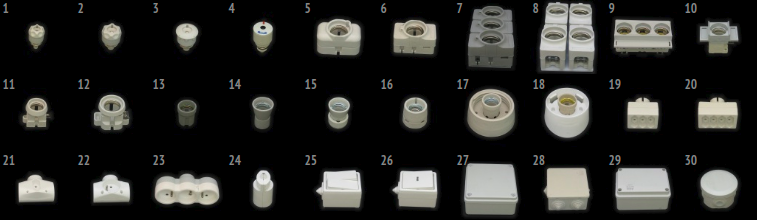
\includegraphics[width=0.8\textwidth, trim=0px 0px 0px -20px, clip] {pics/atwork/objects/t-less.png} 
\caption[T-less dataset objects (http://cmp.felk.cvut.cz/t-less/)]{T-less dataset }
\label{fig:labelHere}
\end{figure}

%--------------------------------------------------------------------


\begin{figure}[hh!t]
\centering
\subfigure[]{
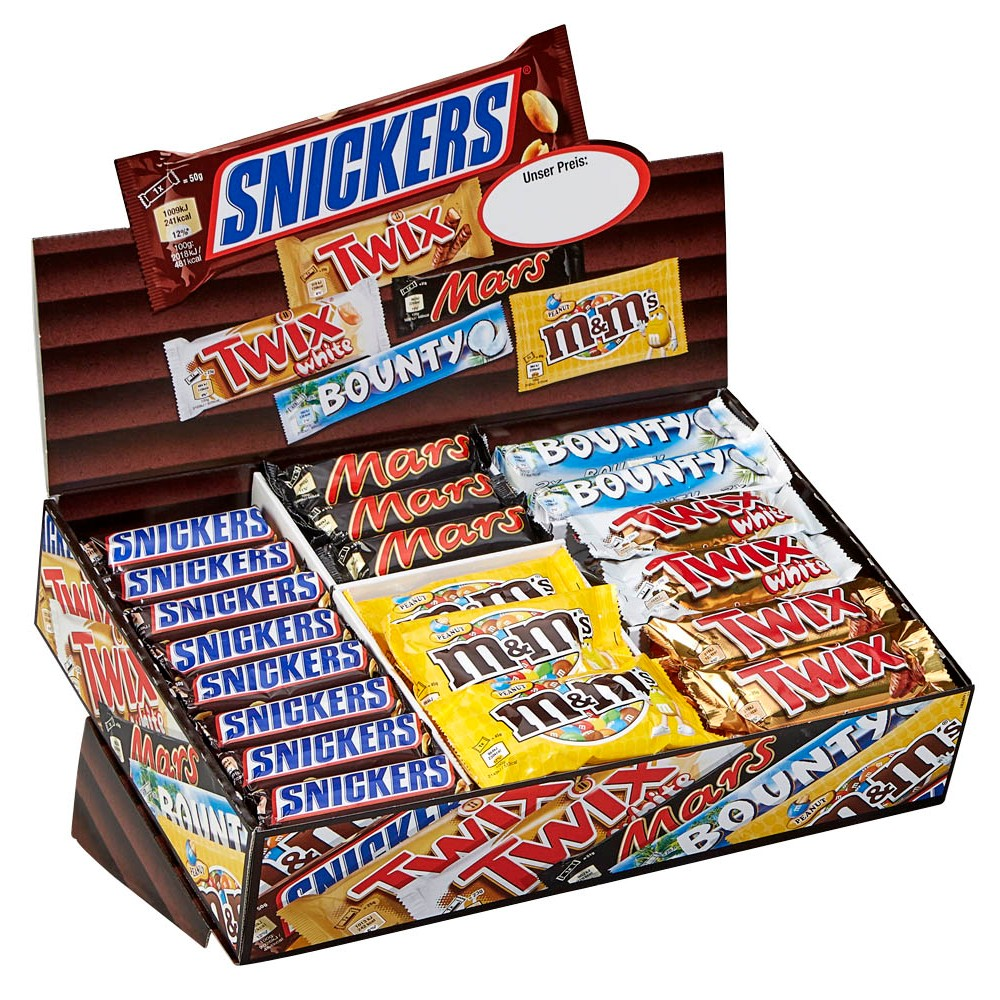
\includegraphics[width=0.3\textwidth, trim=0px 0px 0px -20px, clip] {fig/workObjects/all.jpeg}
   \label{fig:subfig1}
}
\subfigure[]{
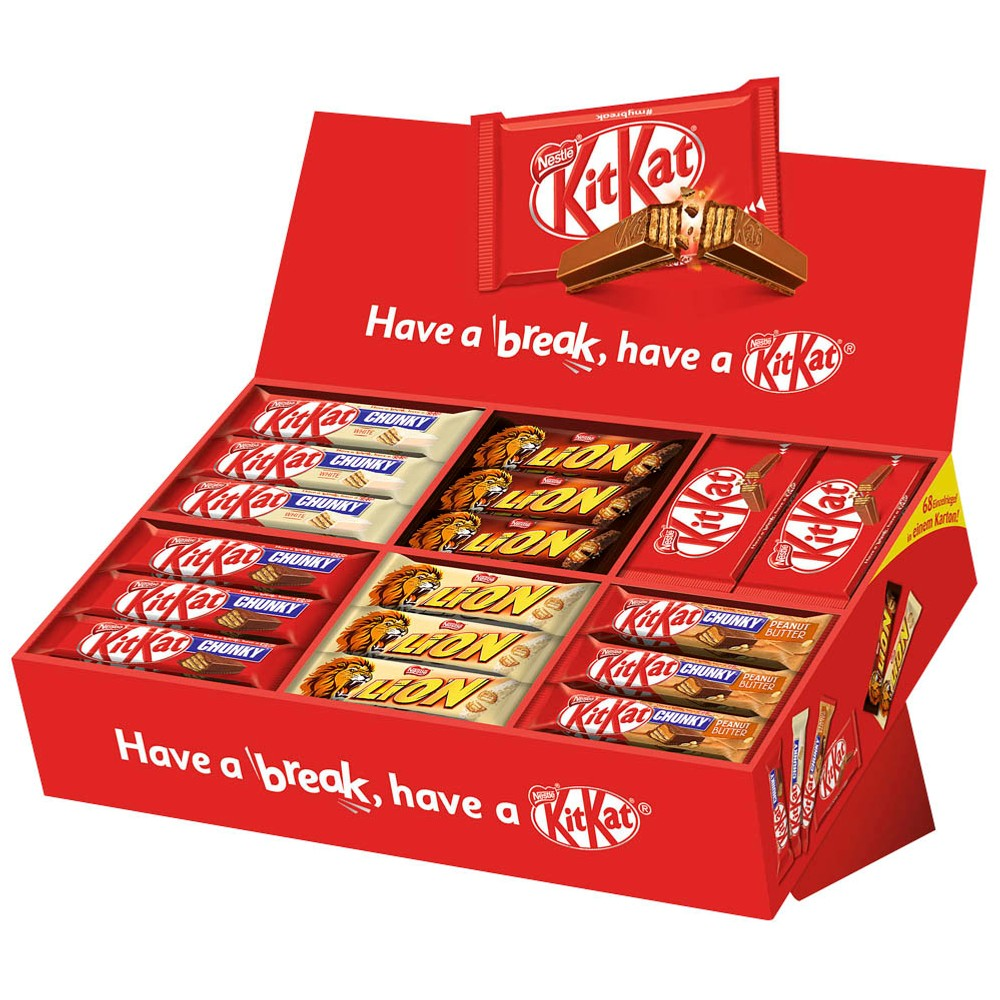
\includegraphics[width=0.3\textwidth, trim=0px 0px 0px -20px, clip] {fig/workObjects/nestle.jpeg}
   \label{fig:subfig2}
}
\subfigure[]{
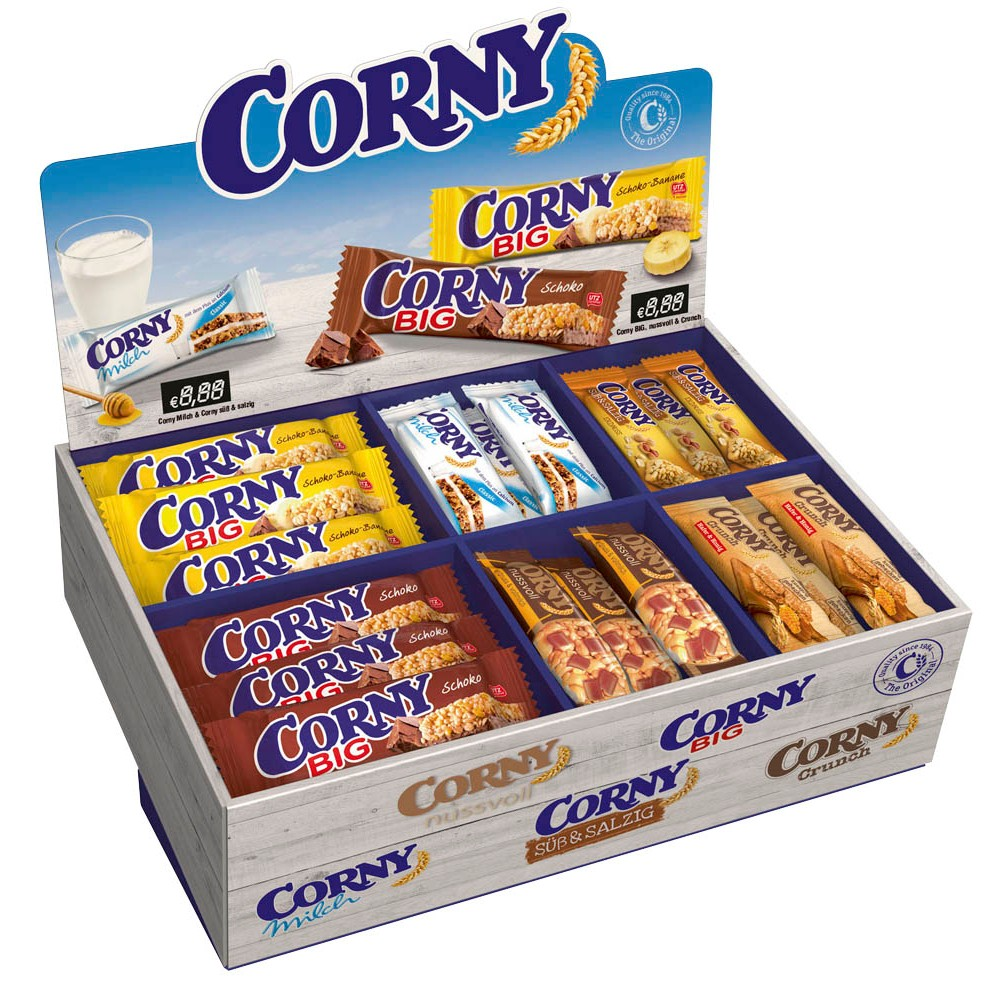
\includegraphics[width=0.3\textwidth, trim=0px 0px 0px -20px, clip] {fig/workObjects/corny.jpeg}
   \label{fig:subfig3}
}
\caption[Chocolate Objects (https://www.sweet24.de/)]{Chocolate objects }
\label{fig:labelHere}
\end{figure}
%--------------------------------------------------------------------
% EOF
%--------------------------------------------------------------------

%%!TEX root = ./ERL Industrial Robots.tex

%--------------------------------------------------------------------
%--------------------------------------------------------------------
\subsection{Identifier}
\label{ssec:Identifier}

The identifier consists of the information about the object class, the object type and the unique identifier.
Each information in the identifier is separated by a single dash.
For example EM-01-01 means that the object is of class EM (objects in the environment to manipulate), it is of type 01
(assembly aid tray) and it is the object ``01''.
The identifier is used to monitor the production process and as a reference number to track customer specific assemblies.
\erlir uses ArUco marker (size of approximately $2.5cm\times2.5cm$) as an identifier for areas and objects in its environment. 
For example ArUco marker id ``1'' is mapped to EM-01-01 which is the identifier for one of the assembly aid trays available in the environment. 
Table \ref{tab:ObjectID} and \ref{tab:AreaID} show the identifier of each object and area in the \erlir environment.

\begin{longtable}{|l|l|l|}
\caption{Objects ID}
\label{tab:ObjectID}
\\ \hline
\textbf{Object} & \textbf{Object ID} & \textbf{Marker ID}\\ 
  \hline 
Assembly aid tray & EM-01-01 & 1 \\ \cline{2-3}
& EM-01-02 & 2 \\ \cline{2-3}
&  EM-01-02 & 3 \\ \hline 
File card box & EM-02-01 & 21 \\ \cline{2-3}
 & EM-02-02 & 22 \\ \cline{2-3}
& EM-02-03 & 23 \\ \hline
Container Box& ER-02-01 & 61 \\ \cline{2-3}
(ER-02-01 -> ER-02-10) & ER-02-02 & 62 \\ \cline{2-3}
& ER-02-03 & 63 \\ \cline{2-3}
& ER-02-04 & 64 \\ \cline{2-3}
& ... & ...  \\ \cline{2-3}
& ER-02-08 & 68 \\ \cline{2-3}
& ER-02-09 & 69 \\ \cline{2-3}
& ER-02-10 & 70 \\ \hline 
\end{longtable} 		

\newpage

\begin{longtable}{|l|l|l|}
\caption{Area ID}
\label{tab:AreaID}
\\ \hline
\textbf{Object} & \textbf{Object ID} & \textbf{Marker ID}\\ 
  \hline 
Shelves & SH-01 & 81 \\ \cline{2-3}
(SH-01 -> SH-24) & SH-02 & 82 \\ \cline{2-3}
& SH-03 & 83 \\ \cline{2-3}
& ... & ... \\ \cline{2-3}
& SH-22 & 102 \\ \cline{2-3}
& SH-23 & 103 \\ \cline{2-3}
& SH-24 & 104 \\ \hline
Drilling workstation & WS-01 & 131 \\ \cline{2-3}
& WS-02 & 132 \\ \hline
Force fitting workstation & WS-03 & 133 \\ \cline{2-3}
& WS-04 & 134 \\ \hline
Assembly workstation & WS-05 & 135 \\ \cline{2-3}
& WS-06 & 136 \\ \cline{2-3}
& WS-07 & 137 \\ \hline
Conveyor belt & CB-01 & 161 \\ \hline
Drilling machine & DM-01 & 162 \\ \hline
\end{longtable} 		

%!TEX root = ./ERL Industrial Robots.tex


%--------------------------------------------------------------------
%--------------------------------------------------------------------
\subsection{Networked Devices in the Environment}
\label{ssec:NetworkedDevices}
There are various networked devices available in the \erlir environment. 
The following description provides an overview on the capability of each networked device.
An interface description for each networked device is provided in detail in the task benchmark section (see Section \ref{sec:TaskBenchmarks}).
Both networked devices are used for delivering parts to the \erlir arena and they are operated by the referee(s).


\begin{figure}[htb]
	\begin{center}
%		\hfill
%		\subfigure[Drilling machine]{
%			\scalebox{1.0}[1.0]{
%				\includegraphics[height=28mm,angle=90,trim=0px 0px 0px 0px,clip]%
%				{pics/atwork/networked_devices/drillingMachine.jpg}%
%			}
%			\label{fig:nutshellcoverPlateDrillingMachine}
%		}%
		\hfill
		\subfigure[Conveyor belt]{
			\scalebox{1.0}[1.0]{%
				\includegraphics[height=28mm,angle=90,trim=0px 0px 0px 0px,clip]%
				{pics/atwork/networked_devices/QCC.jpg}%
			}%
			\label{fig:nutshellcoverPlateQCC}
		}%
%		\hfill
%		\subfigure[Force fitting machine]{
%			\scalebox{1.0}[1.0]{%
%				\includegraphics[height=28mm,angle=90,trim=0px 0px 0px 0px,clip]%
%				{pics/atwork/networked_devices/forceFittingMachine.jpg}%
%			}%
%			\label{fig:nutshellForceFittingMachine}
%		}%
		\hfill
		\subfigure[Rotating table]{
			\scalebox{1.0}[1.0]{%
				\includegraphics[height=28mm,angle=0,trim=0px 0px 0px 0px,clip]%
				{pics/atwork/networked_devices/rotatingTable.jpg}%
			}%
			\label{fig:nutshellForceFittingMachine}
		}%
		\hfill\mbox{}
		\caption{Networked devices within the \erlir environment.}
		\label{fig:NutshellNetworkedDevices} 
	\end{center}
\end{figure}

%	\item \emph{Force fitting machine.}
%	The force fitting machine is used for the insertion of a bearing into a bearing box.
%	The force fitting process is performed by first inserting a bearing box with bearing on top of the bearing box. 
%	The placement process is executed with the help of an assembly aid tray.
%	After the bearing box and bearing is properly placed, the force fitting machine is instructed to move down. 
%	Finally, the force fitting machine is instructed to move up again and the processed bearing box and bearing can be picked up (Figure \ref{fig:RoawNetForceFit}).
%	The force fitting machine is used in the \emph{prepare assembly aid tray for force fitting} task.
%\begin{figure}[htb]
%  \begin{center}
%	  \hfill
%		 \subfigure[]{
%		  \scalebox{1.0}[1.0]{
%  		  \includegraphics[height=35mm,angle=90,trim=450px 50px 0px 0px,clip]
%	  		{fig/forceFittingMachine.jpg}
%			}
%			\label{fig:RoawNetForceFit2}
%		}
%  	  \hfill
%	  \subfigure[]{
%		  \scalebox{1.0}[1.0]{
%  		  \includegraphics[height=40mm,angle=0,trim=0px -250px 0px 0px,clip]
%	  		{fig/roawTBM1.jpg}
%			}
%		   \label{fig:RoawNetForceFit1}
%		}
%		\hfill\mbox{}
%	  \caption{The \erlir force fitting machine (a) and bearing boxes in the middle of force fitting process (b). The first bearing (right side) has been successfully force fitted into a bearing box.}
%  	\label{fig:RoawNetForceFit} 
%	\end{center}
%\end{figure}

%	\item \emph{Drilling machine.}
%	The drilling machine is used for drilling a cone sink in a cover plate.
%	The drilling machine is equipped with a customized fixture for the plates.
%	Similar to the force fitting machine, the drilling machine is operated by first inserting the cover plate into the fixture of the drilling machine. 
%	The cover plate placement is followed by moving the drill head down.
%	Finally, the drill is moved up again and the drilled cover plate can be picked up.
%	The drilling machine is used in the plate drilling task specifically in the correction of a faulty cover plate.
%\begin{figure}[htb]
%  \begin{center}
%	  \hfill
%		 \subfigure[]{
%		  \scalebox{1.0}[1.0]{
%  		  \includegraphics[height=35mm,angle=90,trim=0px 0px 0px 0px,clip]
%	  		{fig/drillingMachine.jpg}
%			}
%			\label{fig:RoawNetDrill1}
%		}
%  	  \hfill
%	  \subfigure[]{
%		  \scalebox{1.0}[1.0]{
%  		  \includegraphics[height=52mm,angle=0,trim=900px 150px 150px 250px,clip]
%	  		{fig/roawTBM2.jpg}
%			}
%		   \label{fig:RoawNetDrill2}
%		}
%		\hfill\mbox{}
%	  \caption{The \erlir drilling machine (a) and a cover plate which is placed in the fixture of the drilling machine (b).}
%  	\label{fig:RoawNetDrill} 
%	\end{center}
%\end{figure}




%\item \emph{Quality control camera.} 
%The quality control camera or QCC is placed on top of the conveyor belt and it is used to acquire information on the quality of incoming cover plates delivery through the conveyor belt. 
%The QCC has the responsibility to deliver one cover plate through the conveyor belt (until the cover plate reaches the exit ramp of the conveyor belt) for each received command.
%After receiving a command, the QCC operates the conveyor belt until a cover plate is within the QCC range of view where the QCC will detect any defects on the cover plate.
%The conveyor belt will keep moving until it is stopped by QCC when the cover plate is at the exit ramp of the conveyor belt.
%The QCC it is used for the plate drilling task.


%--------------------------------------------------------------------
% EOF
%--------------------------------------------------------------------

%!TEX root = ./ERL Industrial Robots-rulebook.tex

%--------------------------------------------------------------------
%--------------------------------------------------------------------
\subsection{Central Factory Hub}
\label{ssec:CFH}

The main idea of the \erlir testbed software infrastructure is to have a central server-like hub (the \erlir \CFH) that serves all the services that are needed for executing and scoring tasks and successfully realize the competition. This hub is derived from software systems well known in industrial business (e.g. SAP). It provides the robots with information regarding the specific tasks and tracks the production process as well as stock and logistics information of the \rollin factory. It is a plug-in driven software system. Each plug-in is responsible for a specific task, benchmarking or other functionality.

\noindent
The following set of specifications must be met by the \erlir \CFH (CFH).
%-----------
\begin{CFHSpec}[Central Factory Hub]
Central managing of all services needed for controlling data, devices and robots. In the following paragraphs, several plug-in will be described. In future, a web-based user interface would be useful.
\end{CFHSpec}

%-----------
\begin{CFHSpec}[Benchmarking Plug-in]
A plug-in to serve general benchmark functionalities or interact with a separated BM software.
\end{CFHSpec}

%-----------
\begin{CFHSpec}[Production Tracking Database Plug-in]
An automatic plug-in with the central database tracking all identifiers, status of finished products, sub-assemblies, stock level etc. 
\end{CFHSpec}

The CFH-related sources and client example can be obtained from the following locations:

\begin{itemize}
	\item CFH: \url{https://github.com/industrial-robotics/atwork_central_factory_hub}
	\item Client example: \url{https://github.com/industrial-robotics/atwork_refbox_ros_client}
\end{itemize}

%--------------------------------------------------------------------
% EOF
%--------------------------------------------------------------------

%!TEX root = ./ERL Industrial Robots.tex

%--------------------------------------------------------------------
%--------------------------------------------------------------------
\subsection{Benchmarking Equipment in the Environment}
\label{ssec:BenchmarkingEquipment}

\erlir benchmarking is based on the processing of data collected in two ways:
\begin{itemize}
\item \textbf{internal benchmarking data}, collected by the robot system 
	under test (see Section \ref{sec:RobotsTeams});
\item \textbf{external benchmarking data}, collected by the equipment 
	embedded into the testbed.
\end{itemize}
External benchmarking data is generated by the \erlir testbed with a multitude of methods, depending on their nature.

One of the types of external benchmarking data used by \erlir are pose data about robots and/or their constituent parts. To acquire these, \erlir uses a camera-based commercial motion capture system (e.g. NaturalPoint OptiTrack), composed of dedicated hardware and software. Benchmarking data has the form of a time series of poses of rigid elements of the robot (such as the base or the wrist). There is a case where the motion capture system influences the robot perception system. It is the teams' responsibility to check this effect and coordinate with the benchmarking team in order to minimize this effect. Once generated by the OptiTrack system, pose data are acquired and logged by a customized external software system based on ROS (Robot Operating System): more precisely, logged data is saved as \emph{bagfiles} created with the \emph{rosbag} utility provided by ROS. Pose data is especially significant because it is used for multiple benchmarks. There are other types of external benchmarking data that \erlir acquires: however, these are usually collected using devices that are specific to the benchmark. For this reason, such devices are described in the context of the associated benchmark, rather than here. 

Finally, equipment to collect external benchmarking data includes any \emph{server} which is part of the testbed and that the robot subjected to a benchmark has to access as part of the benchmark. Communication between servers and robot is performed via the testbed's own wireless network (see Section \ref{ssec:RobotBenchEquip}).

%--------------------------------------------------------------------
% EOF
%--------------------------------------------------------------------


\clearpage\phantomsection
%!TEX root = ./ERL Industrial Robots.tex


%--------------------------------------------------------------------
%--------------------------------------------------------------------
%--------------------------------------------------------------------
\section{Robots and Teams}
\label{sec:RobotsTeams}
The purpose of this section is twofold: 
\begin{enumerate}
\item It specifies information about various robot features that can be derived from the environment and the targeted tasks. These features are to be considered at least as desirable, if not required for a proper solution of the task. Nevertheless, we will try to leave the design space for solutions as large as possible and to avoid premature and unjustified constraints.
\item The robot features specified here should be supplied in detail for any robot participating in the competition. This is necessary in order to allow better assessment of competition and benchmark results later on. 
\end{enumerate}

The description of the robot should be included in the team description paper.

\subsection{General Specifications and Constraints on Robots and Teams}
\label{ssec:RobotSpecification}

%-----------
\begin{robotSpec}[System]
A competing team may use a single robot or multiple robots acting as a team.
It is not required that the robots are certified for industrial use.
At least one of the robots entered by a team is capable of:
\begin{itemize}
\item mobility and autonomous navigation. 
\item manipulate and grasp at least several different task-relevant objects. The specific kind of manipulation and grasping activity required is to be derived from the task specifications.
\end{itemize}
The robot subsystems (mobility, manipulation and grasping) should work with the environment and objects specified in this rule book.
\end{robotSpec}

%-----------
\begin{robotSpec}[Sensor Subsystems]
Any robot used by a team may use any kind of \textbf{onboard} sensor subsystem, provided that the sensor system is admitted for use in the general public, its operation is safe at all times, and it does not interfere with other teams or the environment infrastructure. 
A team may use the sensor system in the environment provided by the organizer by using a wireless communication protocol specified for such purpose. Sensor systems used for benchmarking and any other systems intended for exclusive use of the organizers are not accessible by the robot system. 
Teams are not allowed to modify the environment or to install their own embedded devices in the environment, e.g., additional sensors or actuators.
\end{robotSpec}


%-----------
\begin{robotSpec}[Communication Subsystems]
	Any robot used by a team may \textbf{internally} use any kind of communication subsystem, provided that the communication system is admitted for use in the general public, its operation is safe at all times, and it does not interfere with other teams or the environment infrastructure.
	A robot team must be able to use the communication system provided \textbf{as part of the environment} by correctly using a protocol specified for such purpose and provided as part of the scenario. 
\end{robotSpec}


%-----------
\begin{robotSpec}[Power Supply]
	Any mobile device (esp.~robots) must be designed to be usable with an onboard power supply (e.g.~a battery). The power supply should be sufficient to guarantee electrical autonomy for a duration exceeding the periods foreseen in the various benchmarks, before recharging of batteries is necessary.	
	Charging of robot batteries must be done outside of the competition environment. The team members are responsible for safe recharging of batteries. 
	If a team plans to use inductive power transmission devices for charging the robots, they need to request permission from the event organizers in advance and at least three months before the competition. 
	Detailed specifications about the inductive device need to be supplied with the request for permission. 
\end{robotSpec}

%-----------
\begin{robotConstraint}[Computational Subsystems]
	Any robot or device used by a team as part of their solution approach must be suitably equipped with computational devices (such as onboard PCs, microcontrollers, or similar) with sufficient computational power to ensure safe autonomous operation. 
	Robots and other devices may use external computational facilities, including Internet services and cloud computing to provide richer functionalities, but the safe operation of robots and devices may not depend on the availability of communication bandwidth and the status of external services. 	
\end{robotConstraint}
%-----------

\begin{robotConstraint}[Safety and Security Aspects]
	For any device a team brings into the environment and/or the team area, and which features at least one actuator of any kind (mobility subsystems, robot manipulators, grasping devices, actuated sensors, signal-emitting devices, etc.), a mechanisms must be provided to immediately stop its operation in case of an emergency (emergency stop). 
	For any device a team brings into the environment and/or the team area, it must guarantee safe and secure operation at all times. 
	Event officials must be instructed about the means to stop such devices operating and how to switch them off in case of emergency situations. 
\end{robotConstraint}

%-----------
\begin{robotConstraint}[Operation]
In the competition, the robot should perform the tasks autonomously.
An external device is allowed for additional computational power.
It must be clear at all times that no manual or remote control is exerted to influence the behavior of the robots during the execution of tasks.
\end{robotConstraint}


%-----------
\begin{robotConstraint}[Environmental Aspects]
  Robots, devices, and apparatus causing pollution of air, such as combustion engines, or other mechanisms using chemical processes impacting the air, are not allowed.
  Robots, devices, and any apparatus used should minimize noise pollution. In particular, very loud noise as well as well-audible constant noises (humming, etc.) should be avoided. The regulations of the country in which a competition or benchmark is taking place must be obeyed at all times. The event organizers will provide specific information in advance, if applicable. Robots, devices, and any apparatus used should not be the cause of effects that are perceived as a nuisance to humans in the environment. Examples of such effects include causing wind and drafts, strong heat sources or sinks, stenches, or sources for allergic reactions. 
\end{robotConstraint}

%--------------------------------------------------------------------
%--------------------------------------------------------------------

\subsection{Benchmarking Equipment in the Robots}
\label{ssec:RobotBenchEquip}

\paragraph{Preliminary Remark:}
Whenever teams are required to install some element provided by \erlir on (or in) their robots, such element will be carefully chosen in order to minimize the work required from teams and the impact on robot performance.

\paragraph{Hardware}
As a general rule, \erlir does not require that teams install additional robotic hardware on their robots. Moreover, permanent change to the robot's hardware is never required. However, \erlir may require that additional standard PC hardware (such as an external, USB-connected hard disk for logging) is temporarily added to the robot in order to collect internal benchmarking data. When this is the case, the additional hardware is provided by \erlir during the competition, and its configuration for use is either automatically performed by the operating system, or very simple.

To allow the acquisition of external benchmarking data about their pose, robots need to be fitted with special reflective markers, mounted in known positions. The teams will be required to prepare their robots to ease the mounting of the markers. Teams will be required to provide the geometric transformation from the position of the marker to the odometric center of the robot\footnote{Benchmarking data related to poses will refer to the marker position: this is why additional information is required to know the position of the base.}.

\paragraph{Software} \erlir may require that robots run \erlir-provided (or publicly available) software during benchmarks. A typical example of such software is a package that logs data provided by the robot, or a client that interfaces with a \erlir server via the wireless network of the testbed. Whenever a team is required to install and run such a package, it will be provided as source code, its usage will be most simple, and complete instruction for installation and use will be provided along with it. All \erlir software is written to have a minimal impact on the performance of a robot, both in terms of required processing power and in terms of (lack of) interaction with other modules. When required by a benchmark, the relevant \erlir software to be run by participating robots is provided well in advance with respect to the competition.

\erlir will make any effort to avoid imposing constraints on the teams participating to the competition in terms of software architecture of their robots. This means that any provided piece of software will be designed to have the widest generality of application. However, this does not mean that the difficulty of incorporating such software into the software architecture of a robot will be independent from such architecture: for technical reasons, differences may emerge. A significant example is that of software for data logging. At the moment, it appears likely that any such software by \erlir will be based on the established \emph{rosbag} software tool, library and file format. As rosbag is part of ROS (Robot Operating System), robots based on ROS can use it to log data without any modification; on the contrary, robots not using ROS will be required to employ the rosbag library to create rosbag files (\emph{bagfiles}) or to develop ad-hoc code to convert their well established logging format into the rosbag one by using the rosbag API. If this will be the case, \erlir will provide tools to ease the introduction of software modules for creation of bagfiles into any software architecture; yet, teams not using ROS will probably have to perform some additional work to use such tools.

\subsection{Robot Communication with Benchmarking Equipment}
\label{ssec:BenchEquipRobotCommunication}
For some types of internal benchmarking data (i.e.~provided by the robot), logging is done on board the robot, and data are collected after the benchmark (for instance, via USB stick). Other types of internal benchmarking data, instead, are communicated by the robot to the testbed during the benchmark. In such cases, communication is done by interfacing the robot with standard wireless network devices (e.g. IEEE 802.11n) that are part of the testbed, and which therefore become a part of the benchmarking equipment of the testbed. However, it must be noted that network equipment is not strictly dedicated to benchmarking: for some benchmarks, in fact, the \wifi ~may be (or exclusively) used to perform interaction between the robot and the testbed.

Due to the need to communicate with the testbed via the \wifi, all robots participating to the \erlir competition are required to:
\begin{enumerate}
\item possess a fully functional IEEE 802.11n network interface\footnote{It must be stressed that full functionality requires that the network interface must not be hampered by electromagnetic obstacles, for instance by mounting it within a metal structure and/or by employing inadequate antenna arrangements. Network spectrum in the competition area is typically very crowded, and network equipment with impaired radio capabilities may not be capable of accessing the testbed \wifi, even if correctly working in less critical conditions.};
\item be able to keep the wireless network interface permanently connected to the testbed \wifi \ for the whole duration of the benchmarks.
\end{enumerate}

\subsection{YAML Data File Specification} \label{sssec:YamlDataFileSpec}
The subsequent paragraphs specify the YAML file format that can be converted to ROS bag files. This closely follows the data items described in D-2.1.7 \cite{rockin:D-2.1.7:2014}. The YAML format was chosen because it is a simple format, easy to produce without using any special library. Furthermore, the ROS messages format is already defined: as produced by the \verb!rostopic echo! command.

\subsubsection{File Format}
The YAML file should be composed of a single list of messages. Each message should have four items:
\begin{itemize}
 \item \verb!topic! - The topic name.
 \item \verb!secs! - Timestamp of the message, in number of seconds since 1970.
 \item \verb!nsecs! - Nanoseconds component of the timestamp.
 \item \verb!message! - The message, according to the topic type.
\end{itemize}

The message should be formatted in YAML, according to its structure. This is the same as the output of \verb!rostopic echo!. However, binary fields may be specified in base 64 encoding for much smaller files. You can copy the file \verb!src/base64.hpp! to your project, it depends only on boost to encode base 64.

And example for a file generated according to above specification could look as follows:
\begin{verbatim}
- topic: pose2d
  secs: 1397024209
  nsecs: 156423000
  message:
   x: 5.5
   y: 6
   theta: 6.4
- topic: image
  secs: 1397024210
  nsecs: 53585000
  message:
   header:
     seq: 306
     stamp:
       secs: 1397024210
       nsecs: 53585000
     frame_id: ''
   height: 4
   width: 4
   encoding: bgr8
   is_bigendian: 0
   step: 12
   data:
     !!binary JaU8JY0kGXUIAZ0UDWzgAXjgAb0kIglwbkGsnkWwoiWUfiGUhi2olhmUgc1YRaUw
\end{verbatim}

\subsubsection{YAML-to-ROSbag Conversion Tool}
A tool to convert \erl YAML files into ROS bag files is available at the RoCKIn Github repository:
\begin{center}
	\url{https://github.com/rockin-robot-challenge/benchmark_and_scoring_converter}
\end{center}

%--------------------------------------------------------------------
% EOF
%--------------------------------------------------------------------


%--------------------------------------------------------------------
%--------------------------------------------------------------------
%--------------------------------------------------------------------
\newpage
\section{Task Benchmarks}
\label{sec:TaskBenchmarks}

Details concerning rules, procedures, as well as scoring and benchmarking methods, are common to all task benchmarks.

\begin{description}
\item[Rules and Procedures] Every run of each of the task benchmark will be preceded by a safety-check, outlined as follows:
%
\begin{enumerate}
     \item The team members must ensure and inform at least one of the organizing committee (OC) member, present during the execution of the task, that they have an emergency stop button on the robot which is fully functional. Any member of the OC can ask the team to stop their robot at any time which must be done immediately.
     \item A member of the OC present during the execution of the task will make sure that the robot complies with the other safety-related rules and robot specifications presented in Section~\ref{sec:RobotsTeams}.
\end{enumerate}
%
All teams are required to perform each task according to the steps mentioned in the rules and procedures sub-subsections for the tasks. During the competition, all teams are required to repeat the task benchmarks several times. On the last day, only a selected number of top teams will be allowed to perform the task benchmarks again. Maximum time allowed for one task benchmark is 10 minutes. 

%--------------------------------------------------------------------
\item[Acquisition of Benchmarking Data]
\label{sec:TbmAcquisitionOfData}
Following some general notes on the acquisition of benchmarking data are described. They are valid for all task benchmarks, as well as for the functional benchmarks.

\begin{itemize}
\item{\textbf{Calibration parameters}}
Important! Calibration parameters for cameras must be saved. This must be done for other sensors (e.g., Kinect) that require calibration as well, if a calibration procedure has been applied instead of using the default values (e.g., those provided by OpenNI).

\item{\textbf{Notes on data saving}}
The specific data that the robot must save is described in the benchmark section. In general some data streams (those with the highest bitrate) must be logged only in the time intervals when they are actually used by the robot to perform the activities required by the benchmark. In this way, system load and data bulk are minimized. For instance, whenever a benchmark includes object recognition activities, video and point cloud data must be logged by the robot only in the time intervals when it is actually performing object recognition.

\item{\textbf{Use of data}}
The logged data is not used during the competition. In particular, it is not used for scoring. The data is processed by \erl consortium members after the end of the competition. It is used for in-depth analysis and/or to produce datasets to be published for the benefit of the robotics community.

\item{\textbf{Where and when to save data}}
Robots must save the data as specified in the section ``Acquisition of Benchmarking Data'' of their respective TBM/FBM on a USB stick provided by \erlir staff. The USB stick is given to the team immediately before the start of the benchmark, and must be returned (with the required data on it) at the end of the benchmark. Each time a teams robot executes a benchmark, the team must:

\begin{enumerate}
	\item Create, in the root directory of the USB stick, a new directory named
	\begin{itemize}
		\item NameOfTheTeam\_FBMx\_DD\_HH-MM (for FBM) or
		\item NameOfTheTeam\_TBMx\_DD\_HH-MM (for TBM)
	\end{itemize}
	\item Configure the robot to save the data files in these directories.
\end{enumerate}

\end{itemize}

In the filenames above $x$ denotes the number of the benchmark, $DD$ is the day of the month and $HH$, $MM$ represent the time of the day (hours and minutes).

All files produced by the robot that are associated with the execution of the benchmark must be written in this directory. Please note that a new directory must be created for each benchmark executed by the robot. This holds true even when the benchmark is a new run of one that the robot already executed.

During the execution of the benchmark, the following data will be collected\footnote{In the following, `offline' identifies data produced by the robot, and stored locally on the robot, that will be collected by the referees when the execution of the benchmark ends (e.g., as files on a USB stick), while `online' identifies data that the robot has to transmit to the CFH during the execution of the benchmark. Data marked neither with `offline' nor `online' is generated outside the robot.}. In brackets the expected ROS topics are named. Corresponding data types can be stored in a YAML file (see Section \ref{sssec:YamlDataFileSpec}) or rosbag. Following the list of \textbf{offline data} to be logged:

\begin{table}[h]
	\centering
	\begin{footnotesize}
		\begin{tabular}{|l|l|l|l|}
			\hline
			Topic	&	Type		&	Frame Id		&	Notes \\ \hline\hline
			/rockin/robot\_pose\tablefootnote{The 2D robot pose at the floor level, i.e., $z=0$ and only yaw rotation.} & geometry\_msgs/PoseStamped & /map & 10 Hz \\ \hline
			/rockin/marker\_pose\tablefootnote{The 3D pose of the marker in 6 degrees of freedom.	} & geometry\_msgs\/PoseStamped	& /map & 10 Hz \\ \hline
			/rockin/trajectory\tablefootnote{Trajectories planned by the robot including when replanning.} & nav\_msgs/Path & /map & Each (re)plan \\ \hline
			/rockin/<device>/image\tablefootnote{Image processed for object perception; <device> must be any of stereo\_left, stereo\_right, rgb; if multiple devices of type <device> are available on your robot, you can append "\_0", "\_1", and so on to the device name: e.g., "rgb\_0", "stereo\_left\_2", and so on.} & sensor\_msgs/Image	& /<device>\_frame &  -- \\ \hline
			/rockin/<device>/camera\_info\tablefootnote{Calibration info for /erlir/<device>/image.} & sensor\_msgs/CameraInfo & -- & --\\ \hline
			/rockin/depth\_<id>/pointcloud\tablefootnote{Point cloud processed for object perception; <id> is a counter starting from 0 to take into account the fact that multiple depth camera could be present on the robot: e.g., "depth\_0", "depth\_1", and so on.} & sensor\_msgs/PointCloud2 & /depth\_<id>\_frame & -- \\ \hline
			/rockin/scan\_<id>\tablefootnote{Laser scans, <id> is a counter starting from 0 to take into account the fact that multiple laser range finders could be present on the robot: e.g., "scan\_0", "scan\_1", and so on.} &	sensor\_msgs/LaserScan & /laser\_<id>\_frame	& 10-40Hz \\ \hline
			tf\tablefootnote{The tf topic on the robot; the tf tree needs to contain the frames described in this table properly connected through the /base\_frame which is the odometric center of the robot.} & tf & 	--	& -- \\ \hline
		\end{tabular}
	\end{footnotesize}
\end{table}

Some robots might not have some of the sensors or they might have multiple instances of the previous data (e.g., multiple rgb cameras or multiple laser scanner), in this case you append the number of the device to the topic and the frame (e.g., /erlir/scan\_0 in /laser\_frame\_0). It is possible not to log some of the data, if the task does not require it.

The \textbf{online} data part can be found in the description of the respective benchmark.
%--------------------------------------------------------------------
\item[Communication with CFH]
\label{sec:CommCFH}
The following steps describe the part of the CFH communication that is applicable for all TBMs.

\begin{enumerate}
	\item The robot sends a \textbf{BeaconSignal} message at least every second.
	\item The robot waits for \textbf{BenchmarkState} messages. It starts the benchmark execution when the \emph{phase} field is equal to EXECUTION and the \emph{state} field is equal to RUNNING.
	\item The robot waits for an \textbf{Inventory} message from the CFH (which is continuously sent out by the CFH) in order to receive the initial distribution of objects and their locations in the environment.
	\item The robot waits for an \textbf{Order} message from the CFH (which is sent out continuously by the CFH) in order to receive the actual task, i.e., where the objects should be at the end.
	\item The task benchmark ends when all objects are at their final location as specified in the \textbf{Order} message. After that the robot sends a message of type \textbf{BenchmarkFeedback} to the CFH with the \emph{phase\_to\_terminate} field set to EXECUTION. The robot should do this until the \textbf{BenchmarkState}'s \emph{state} field has changed.
\end{enumerate}

The messages to be sent and to be received can be seen on the Github repository located at \cite{rockin:CFHMessages}.

\item[Scoring and Ranking] 
Evaluation of the performance of a robot according to this task benchmark is based on performance equivalence classes and they are related to the fact that the robot has done the required task or not. 

The criterion defining the performance equivalence class of robots is based on the concept of \emph{tasks required achievements}. While the ranking of the robot within each equivalence class is obtained by looking at the performance criteria. In particular:
%
\begin{itemize}
\item The performance of any robot belonging to performance class N is considered as better than the performance of any robot belonging to performance class $M$ whenever $M<N$
\item Considering two robots belonging to the same class, then a penalization criterion (penalties are defined according to task performance criteria) is used and the performance of the one which received less penalizations is considered as better
\item If the two robots received the same amount of penalizations, the performance of the one which finished the task more quickly is considered as better (unless not being able to reach a given achievement within a given time is explicitly considered as a penalty).
\end{itemize}
%
Performance equivalence classes and in-class ranking of the robots are determined according to three sets:
%
\begin{itemize}
\item A set $A$ of \textbf{achievements}, i.e.,~things that should happen (what the robot is expected to do).
\item A set $PB$ of \textbf{penalized behaviors}, i.e.,~robot behaviors that are penalized, if they happen, (e.g.,~hitting furniture).
\item A set $DB$ of \textbf{disqualifying behaviors}, i.e.,~robot behaviors that absolutely must not happen (e.g.,~hitting people).
\end{itemize}
%
Scoring is implemented with the following 3-step sorting algorithm:
%
\begin{enumerate}
\item If one or more of the elements of set $DB$ occur during task execution, the robot gets disqualified (i.e.~assigned to the lowest possible performance class, called class $0$), and no further scoring procedures are performed.
\item Performance equivalence class $X$ is assigned to the robot, where $X$ corresponds to the number of achievements in set $A$ that have been accomplished.
\item Whenever an element of set $PB$ occurs, a penalization is assigned to the robot (without changing its performance class).
\end{enumerate}
%
One key property of this scoring system is that a robot that executes the required task completely will always be placed into a higher performance class than a robot that executes the task partially. Moreover the penalties do not make a robot change class (also in the case of incomplete task).
%

\item[Penalized Behaviors and Disqualifying Behaviors]
The penalizing behaviors for all task benchmarks are:
\begin{itemize}
\item The robot collides with obstacles in the testbed.
\item The robot drops an object.
\item The robot stops working.
\item The robot accidentally place an object on top of another object.
\end{itemize}
The disqualifying behaviors for all task benchmarks are:
\begin{itemize}
\item The robot damages or destroys the objects requested to manipulate.
\item The robot damages the testbed.
\end{itemize}
The achievements for each task are unique and are described in the respective task benchmark section.

\end{description}

%%!TEX root = ./ERL Industrial Robots.tex

%--------------------------------------------------------------------
%--------------------------------------------------------------------
\subsection{Task \emph{Prepare Assembly Aid Tray for Force Fitting}}
\label{ssec:TaskAssemblyAidTray}

This task serves as an example for collecting and assembling parts from different locations. 
Additionally, the teams can show their robots capability in loading and unloading machines (a well known industrial task).
Figure \ref{fig:AidTrayRack} shows the aid tray rack used in the benchmark. On the side of the aid tray unique identifiers are visible to identify the object.
The aid tray is a container that can store up to two bearing boxes.

\begin{figure}[!htbp]
	\begin{center}
		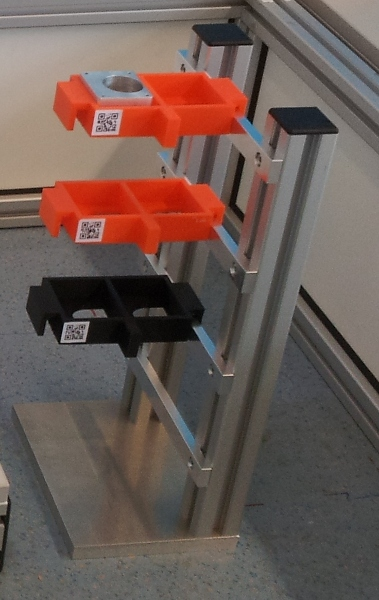
\includegraphics[scale=0.5,angle=0]{pics/atwork/arena_elements/Aid_tray_rack}
		\caption{\roaw Aid tray rack.}
		\label{fig:AidTrayRack}
	\end{center}
\end{figure}

%--------------------------------------------------------------------
\subsubsection{Task Description}
\label{sssec:TaskAssemblyAidTrayDescription}

The robots task is to assist the force fitting process of bearings into bearing boxes with the help of assembly aid tray and force fitting machine. 

%--------------------------------------------------------------------
\subsubsection{Feature Variation}
\label{sssec:TaskAssemblyAidTrayVariation}

The bearing boxes can occur in different shapes (see list of parts in Table \ref{tab:DriveAxlePartsRulebook}). This is caused by a modular concept of the final product where the bearing box has to be inserted in different chassis.
The robots are allowed to collect and insert the bearing boxes in the assembly aid tray individually or collectively.

%--------------------------------------------------------------------
\subsubsection{Input Provided}
\label{sssec:TaskAssemblyAidTrayInput}

The team will be provided with the following information:

\begin{itemize}
\item description of the set of possible assembly aid tray and bearing boxes.
\item description and location(s) of the container(s) used for the bearing boxes.
\end{itemize}

During the execution of the task, the robot should perform the task autonomously and without any additional input.

%--------------------------------------------------------------------
\subsubsection{Expected Robot Behavior or Output}
\label{sssec:TaskAssemblyAidTrayOutput}

The robot navigates to the storage area and collects bearing boxes to be placed into the assembly aid tray.
The robot has the option to deliver the bearing boxes collectively or individually.
After placing the bearing boxes in the assembly aid tray, the robot delivers the assembly aid tray to the force fitting workstation. 
In the force fitting workstation, the assembly aid tray will be processed and the robot will be informed when the process is completed.
The robot will check the final product and can request for another force fitting process when the result is unsatisfactory.

%--------------------------------------------------------------------
\subsubsection{Procedures and Rules}
\label{sssec:TaskAssemblyAidTrayProcedures}

During the execution of this task, which needs to be carried out as per the next steps, an additional robot might be randomly moving in the arena which has to be avoided by the participating robot. 

\begin{description}
     \item [Step 1] The robot, through communicating with the CFH, is provided with multiple assembly aid trays and the information regarding the storage area of the bearing boxes.
     \item [Step 2] Based on the identifier provided beforehand to the teams, the robot must identify the appropriate bearing boxes needed to be put on a tray.
     \item [Step 3] The robot must pick and insert the bearing boxes, identified in Step 2 above, in the provided assembly aid tray.
     \item [Step 4] The robot must deliver the assembly aid tray (with the bearing boxes) to the force fitting workstation to be processed.
\end{description}

%--------------------------------------------------------------------
\subsubsection{Communication to CFH}
\label{sssec:CommCFH}

For this task benchmark the robot does not have to control any networked device in the environment. The force fitting machine will be operated by a human worker. All necessary CFH communication is described in Section \ref{sec:CommCFH}.

%--------------------------------------------------------------------
\subsubsection{Acquisition of Benchmarking Data}
\label{sssec:TaskAssemblyAidTrayData}

General information on the acquisition of benchmarking data is described in Section \ref{sec:TbmAcquisitionOfData}. There, the \textbf{offline} part of the benchmarking data can be found.

\paragraph{Online data}
In order to send online benchmarking data to the CFH, the robot has to use the \textbf{BenchmarkFeedback} message. The message contains:
\begin{itemize}
\item assembly\_aid\_tray\_id (type: string)
\item container\_id (type: string)
\end{itemize}

\paragraph{Offline data} 
The additional information described in the following table has to be logged:

\begin{table}[h]
	\centering
	\begin{footnotesize}
		\begin{tabular}{|l|l|l|l|}
			\hline
			Topic	&	Type		&	Frame Id		&	Notes \\ \hline\hline
			/rockin/qrcode\tablefootnote{ID of the assembly aid tray or container, detected by the robot by analyzing the QR code.} & std\_msgs/Int32 & -- & when recognized \\ \hline
		\end{tabular}
	\end{footnotesize}
\end{table}


%--------------------------------------------------------------------
\subsubsection{Scoring and Ranking}
\label{sssec:TaskAssemblyAidTrayScoring}

Evaluation of the performance of a robot according to this task benchmark is based on performance equivalence classes. Classes are defined in dependence to:

\begin{enumerate}
\item The fact that the robot correctly identifies the assembly aid tray or not;
\item The number of bearing boxes successfully inserted by the robot into the aid tray;
\item The successful execution of the force fitting procedure.
\end{enumerate}

\noindent 
\paragraph{Achievements} The set $A$ of achievements for this task includes:
\begin{itemize}
\item The robot correctly identifies the assembly aid trays identifier.
\item The robot correctly grasps the assembly aid tray.
\item The robot correctly grasps the first bearing box.
\item The robot correctly grasps the second bearing box.
\item The robot inserts the first bearing box into the aid tray.
\item The robot inserts the second bearing box into the aid tray.
\item The robot correctly delivers the tray to the force fitting station.
\item The robot completely processes the first bearing (from identifying to delivering).
\item The robot completely processes the second bearing (from identifying to delivering).
\item The robot cooperates with CFH and Networked Devices throughout the task.
\item The team delivers the benchmarking data appropriately.
\end{itemize}
%--------------------------------------------------------------------
% EOF
%--------------------------------------------------------------------

%%!TEX root = ./ERL Industrial Robots.tex


%--------------------------------------------------------------------
%--------------------------------------------------------------------
\subsection{Task \emph{Plate Drilling}}
\label{ssec:TaskPlateDrilling}



This task simulates handling of an incomplete or faulty parts from an external component supplier. The factory has to quickly react on such issues and create a process to correct the faulty parts.

%--------------------------------------------------------------------
\subsubsection{Task Description}
\label{sssec:TaskPlateDrillingDescription}
The robot has to pick up incoming cover plates and process each cover plate based on its type accordingly.
The robot performs the task with two networked devices in the factory.
The first networked device is the triggered conveyor belt or TCB which is a composite of the quality control camera and the conveyor belt (see Figure \ref{fig:coverPlateQCC}).
The TCB is responsible for delivering the cover plate (by operating the conveyor belt) and detecting the type of the cover plate being delivered.
The second networked device is the drilling machine (see Figure \ref{fig:coverPlateDrillingMachine}) which is operated by the robot to drill a cone sink to the faulty cover plate.

The cover plate of the bearing box has eight holes for connecting the motor with the bearing box and the four central holes need to have a cone sink (see Figure \ref{fig:coverPlatePerfect}). 
There are two possible defects of a cover plate which need to be accommodated in this task.
The first case is where the supplier forgot to drill one of the cone sinks, which results in a faulty cover plate (see Figure \ref{fig:coverPlateFaulty}). 
The faulty cover plates can be corrected by drilling the cone sink with the drilling machine available in the factory.
The second case is where the cover plate is unusable (see Figure \ref{fig:coverPlateUnusable}) and needs to be returned to the supplier for replacement.\\

\begin{figure}[htb]
  \begin{center}
  	\hfill
	  \subfigure[Perfect]{
		  \scalebox{1.0}[1.0]{
  		  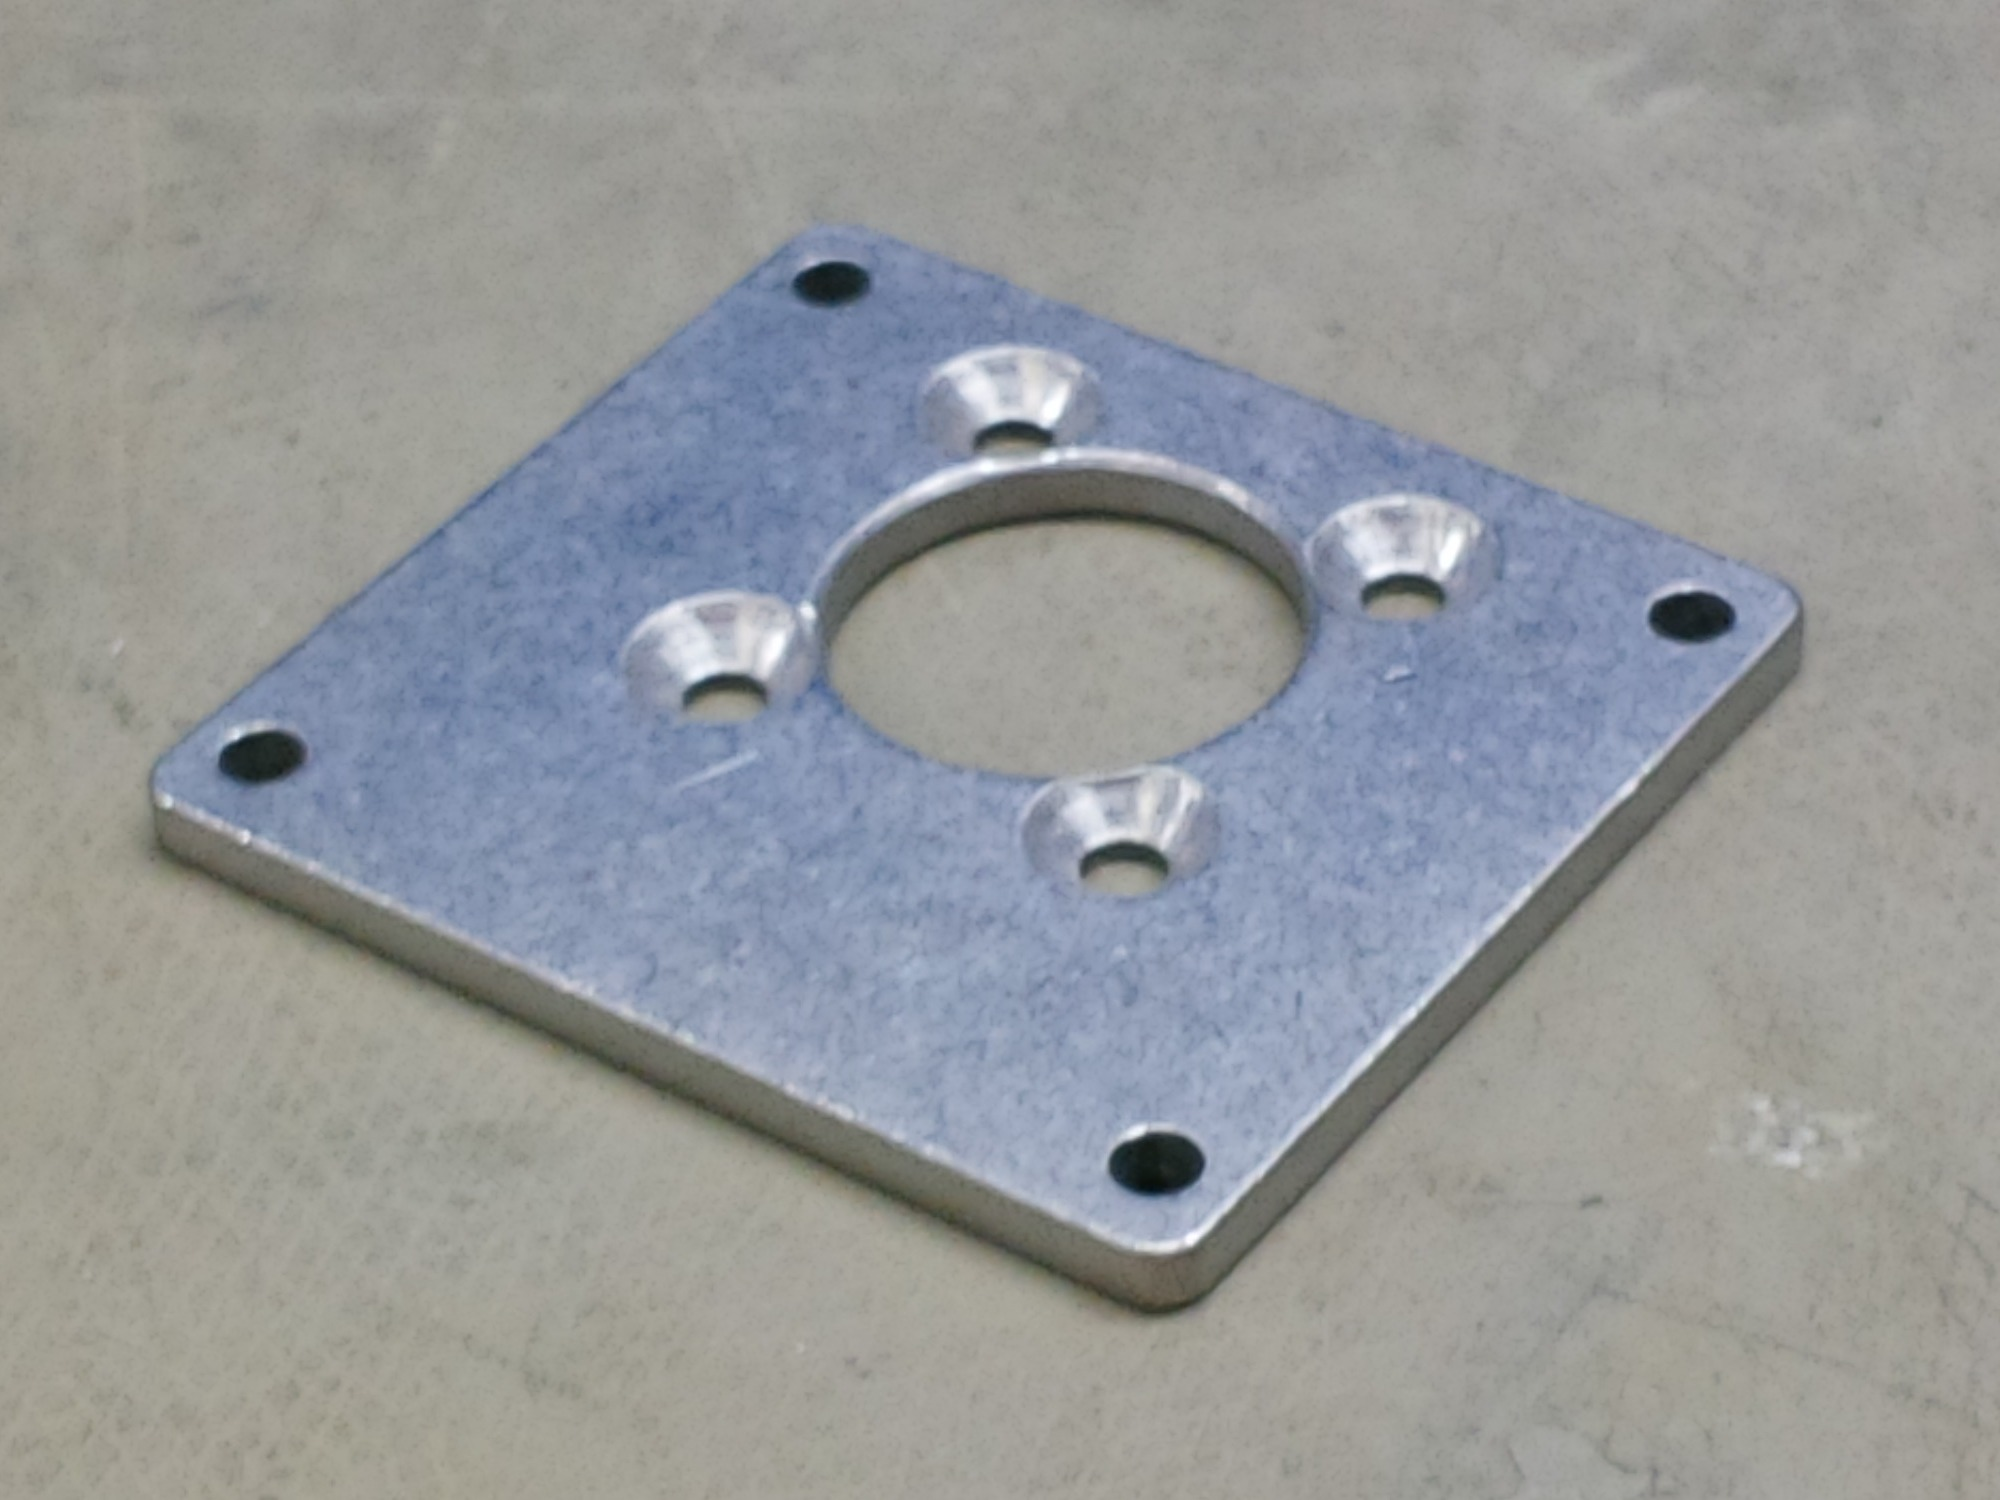
\includegraphics[height=30mm,angle=0,trim=0px 0px 0px 0px,clip]
	  		{./fig/workObjects/cover_plate_perfect.jpg}
			}
		  \label{fig:coverPlatePerfect}
		}
		\hfill
	  \subfigure[Faulty]{
		  \scalebox{1.0}[1.0]{
  		  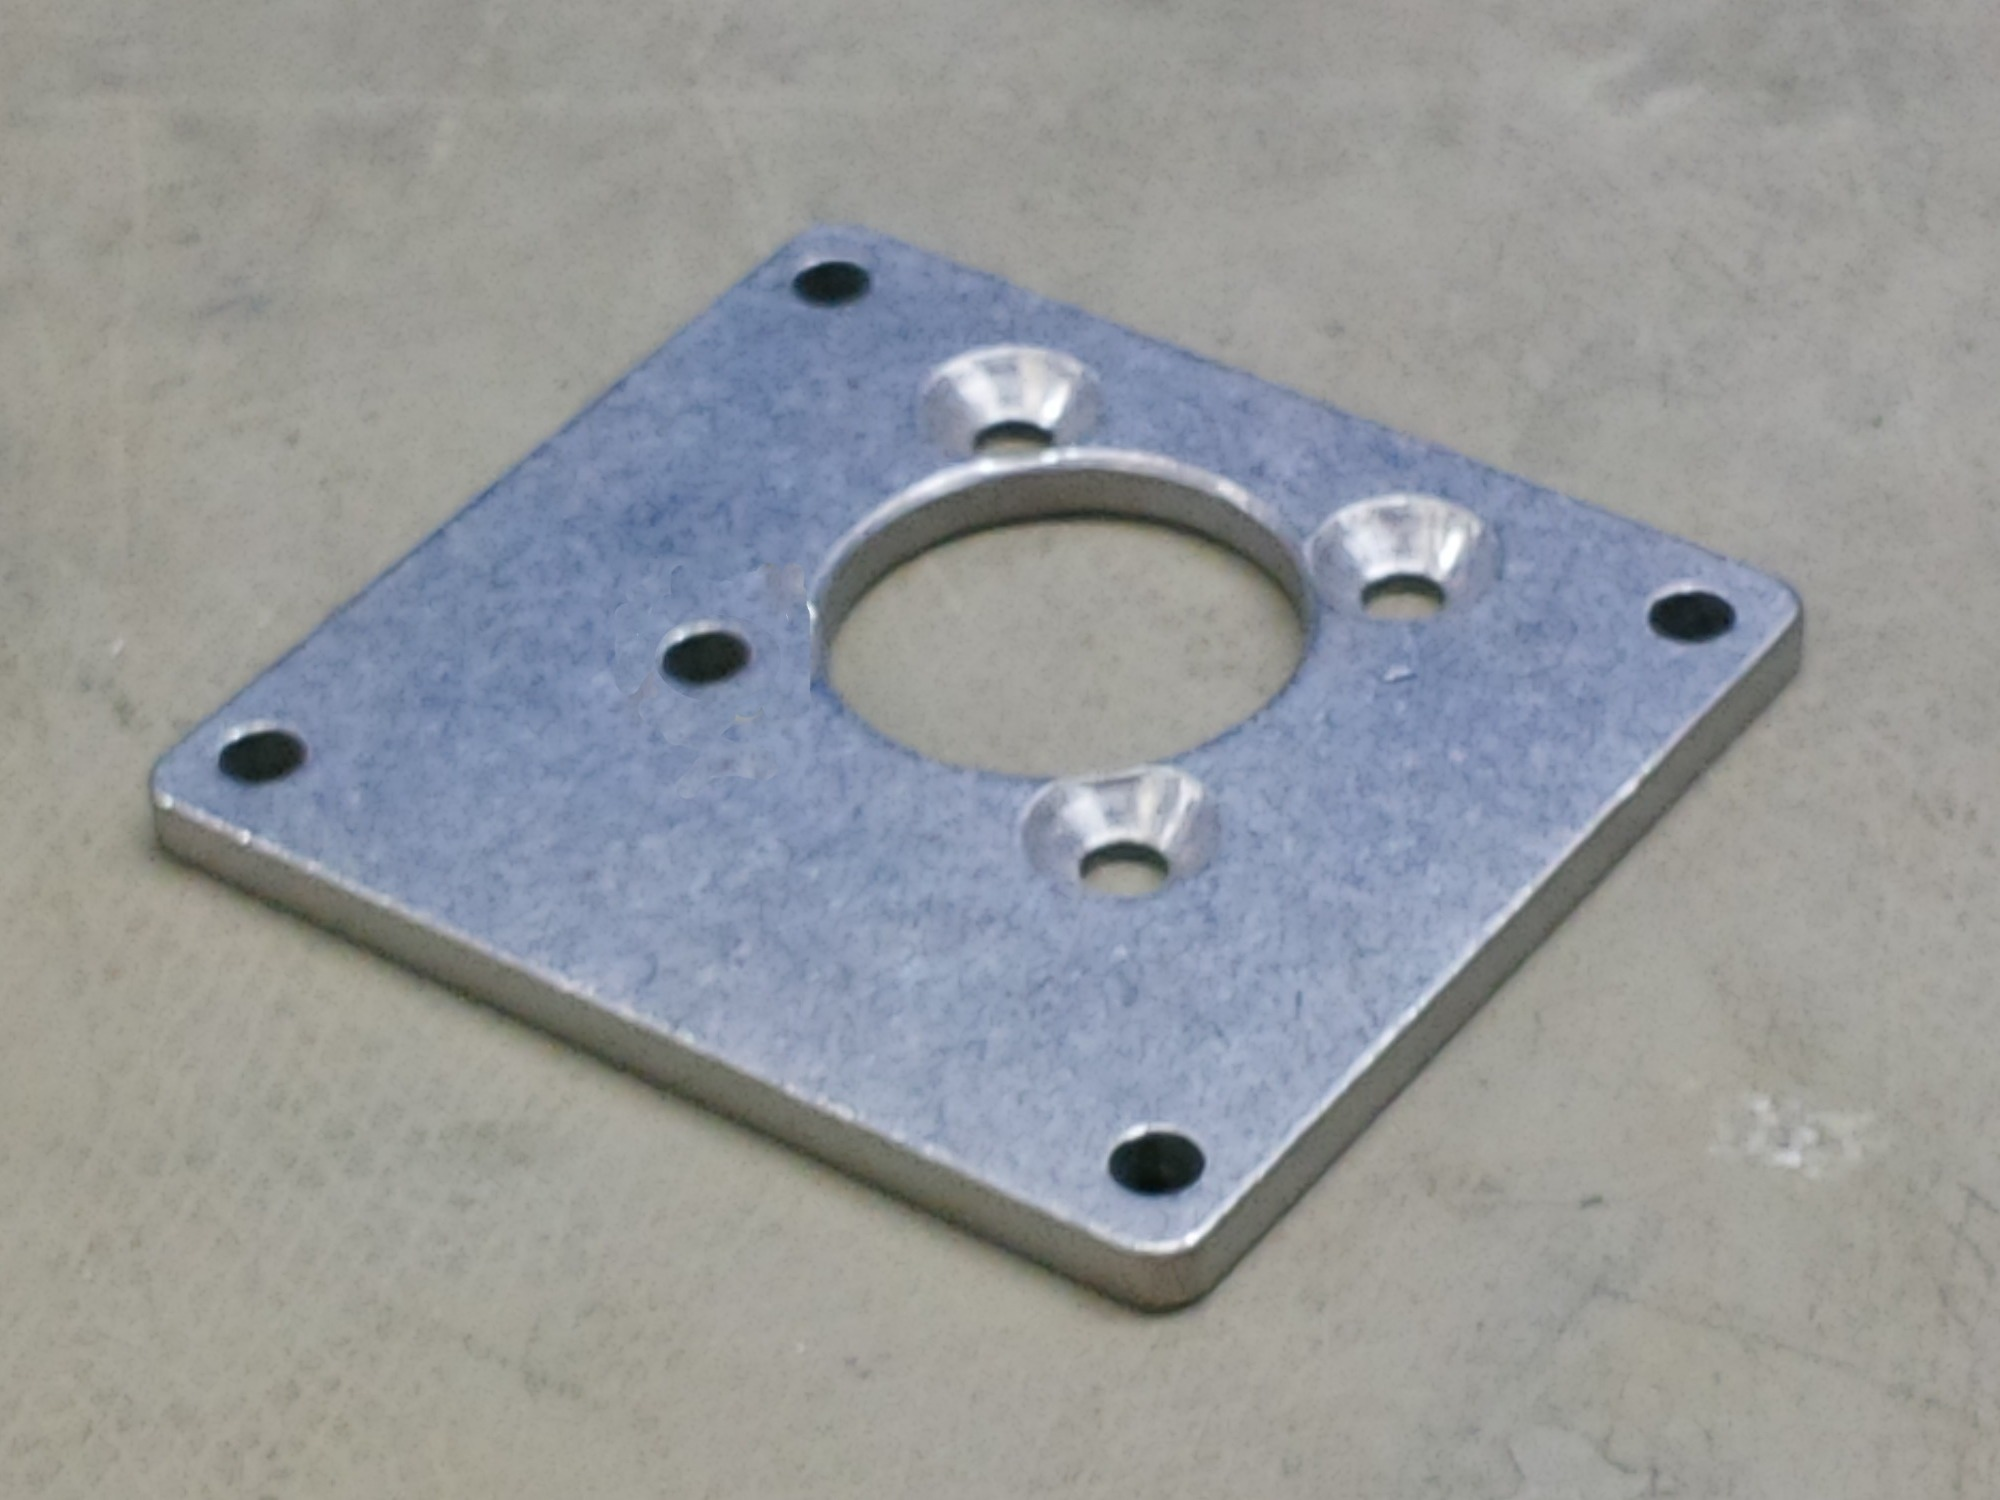
\includegraphics[height=30mm,angle=0,trim=0px 0px 0px 0px,clip]
	  		{./fig/workObjects/cover_plate_faulty.jpg}
			}
		   \label{fig:coverPlateFaulty}
		}
		\hfill
		 \subfigure[Unusable]{
		  \scalebox{1.0}[1.0]{
  		  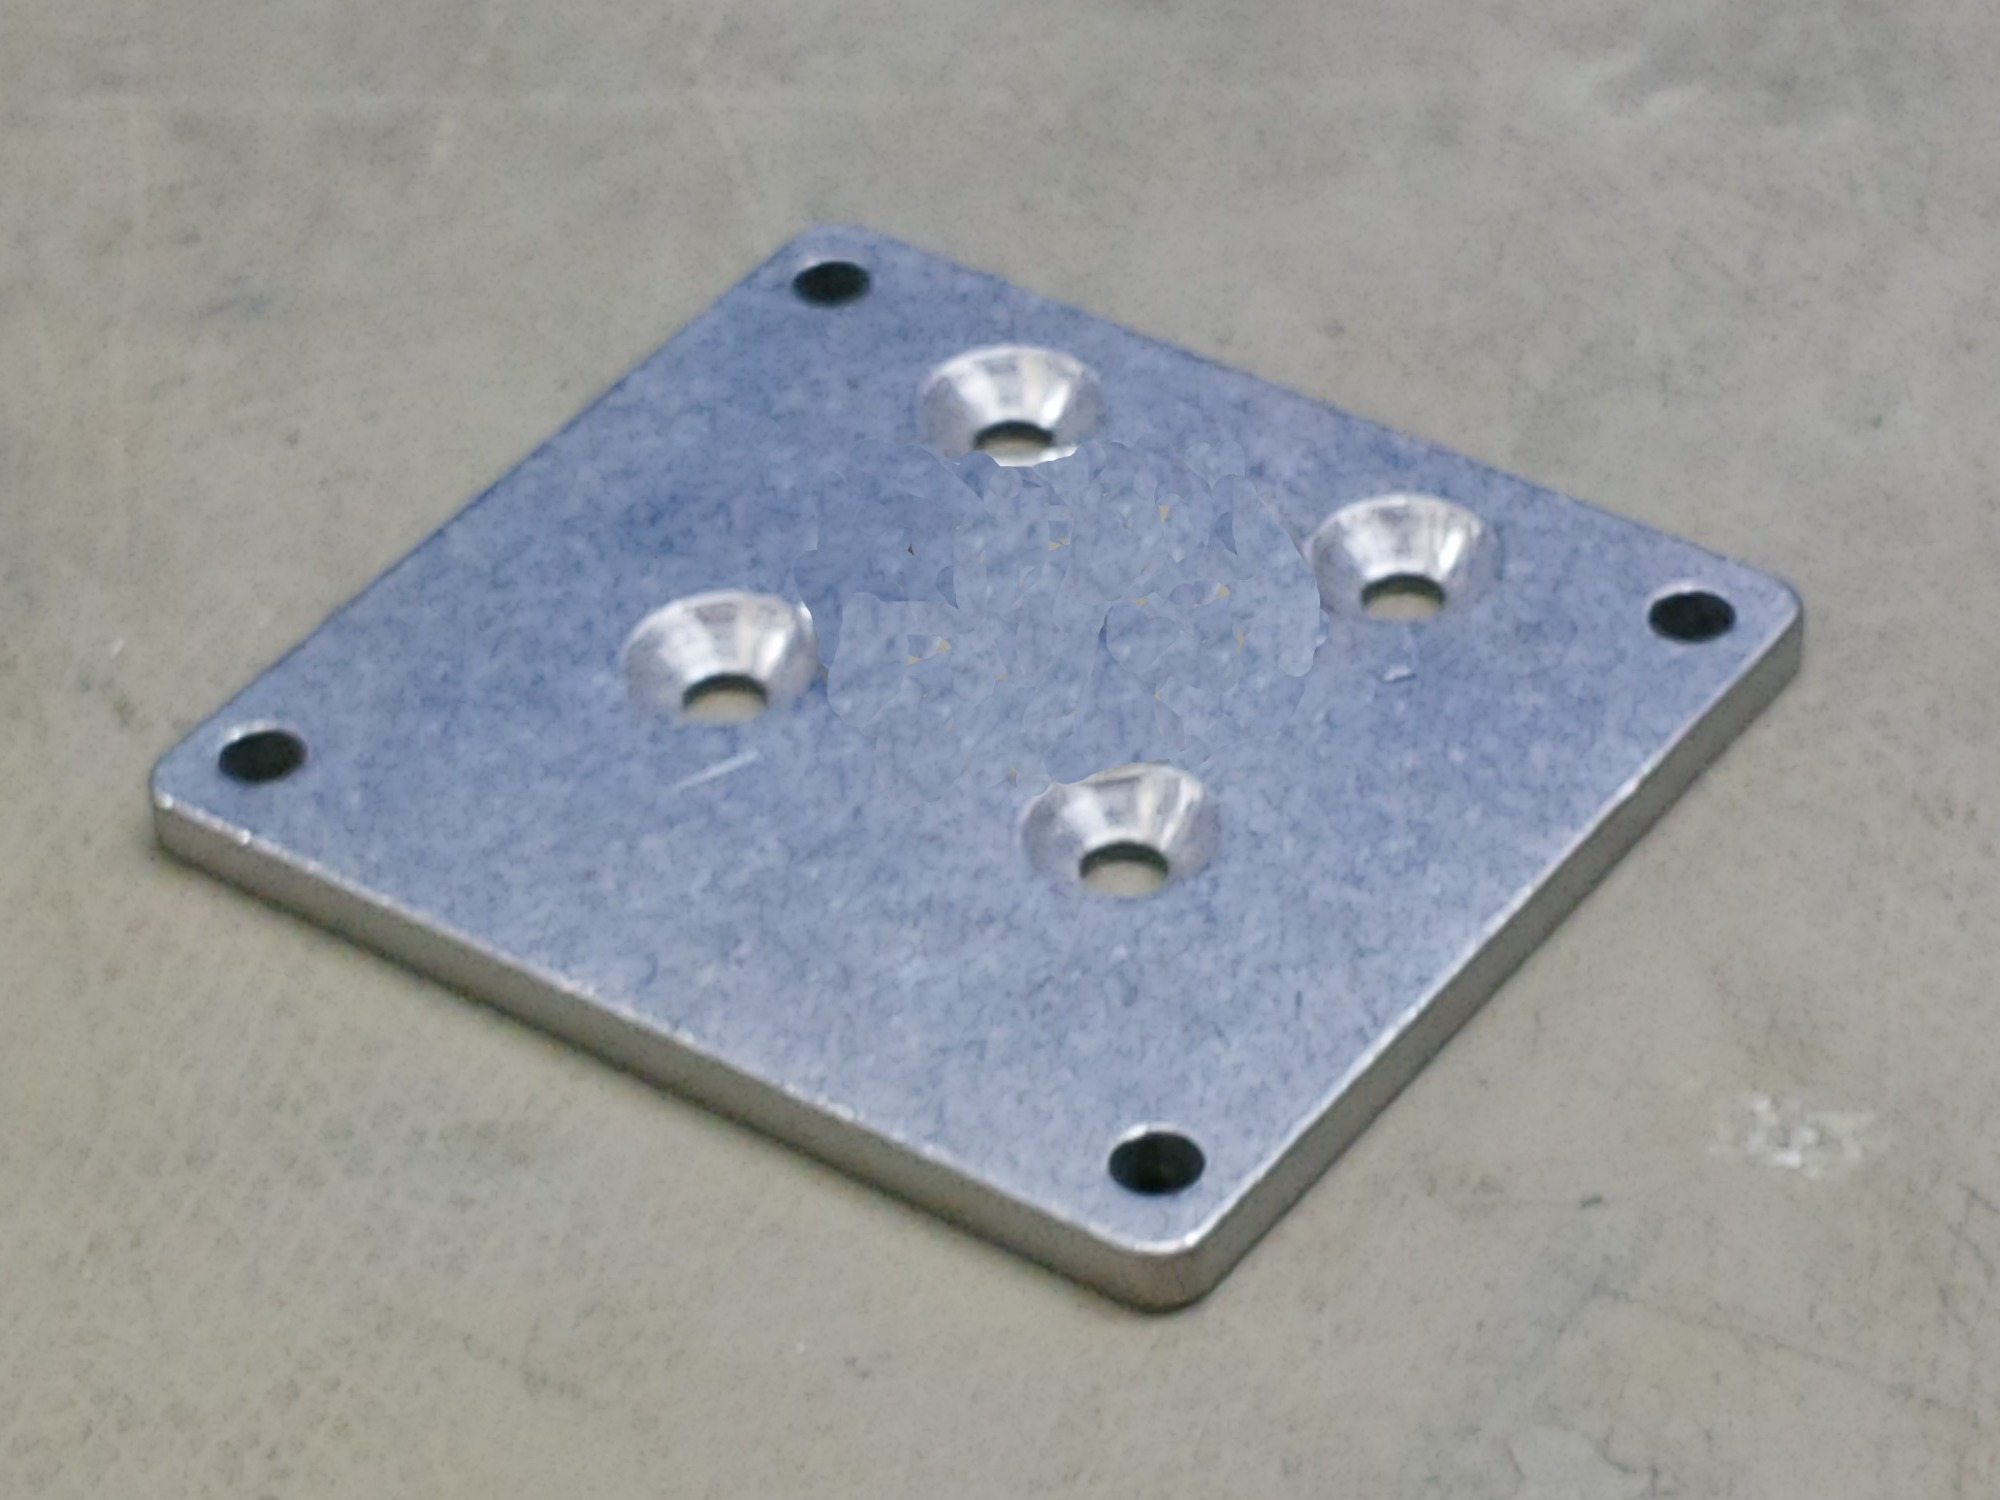
\includegraphics[height=30mm,angle=0,trim=0px 0px 0px 0px,clip]
	  		{./fig/workObjects/cover_plate_unusable.jpg}
			}
			\label{fig:coverPlateUnusable}
		}
		\hfill\mbox{}
	  \caption{Three possible states of the cover plate}
  	\label{fig:coverPlateStates} 
	\end{center}
\end{figure}


\begin{figure}[htb]
  \begin{center}
  	\hfill
	  \subfigure[Drilling machine]{
		  \scalebox{1.0}[1.0]{
  		  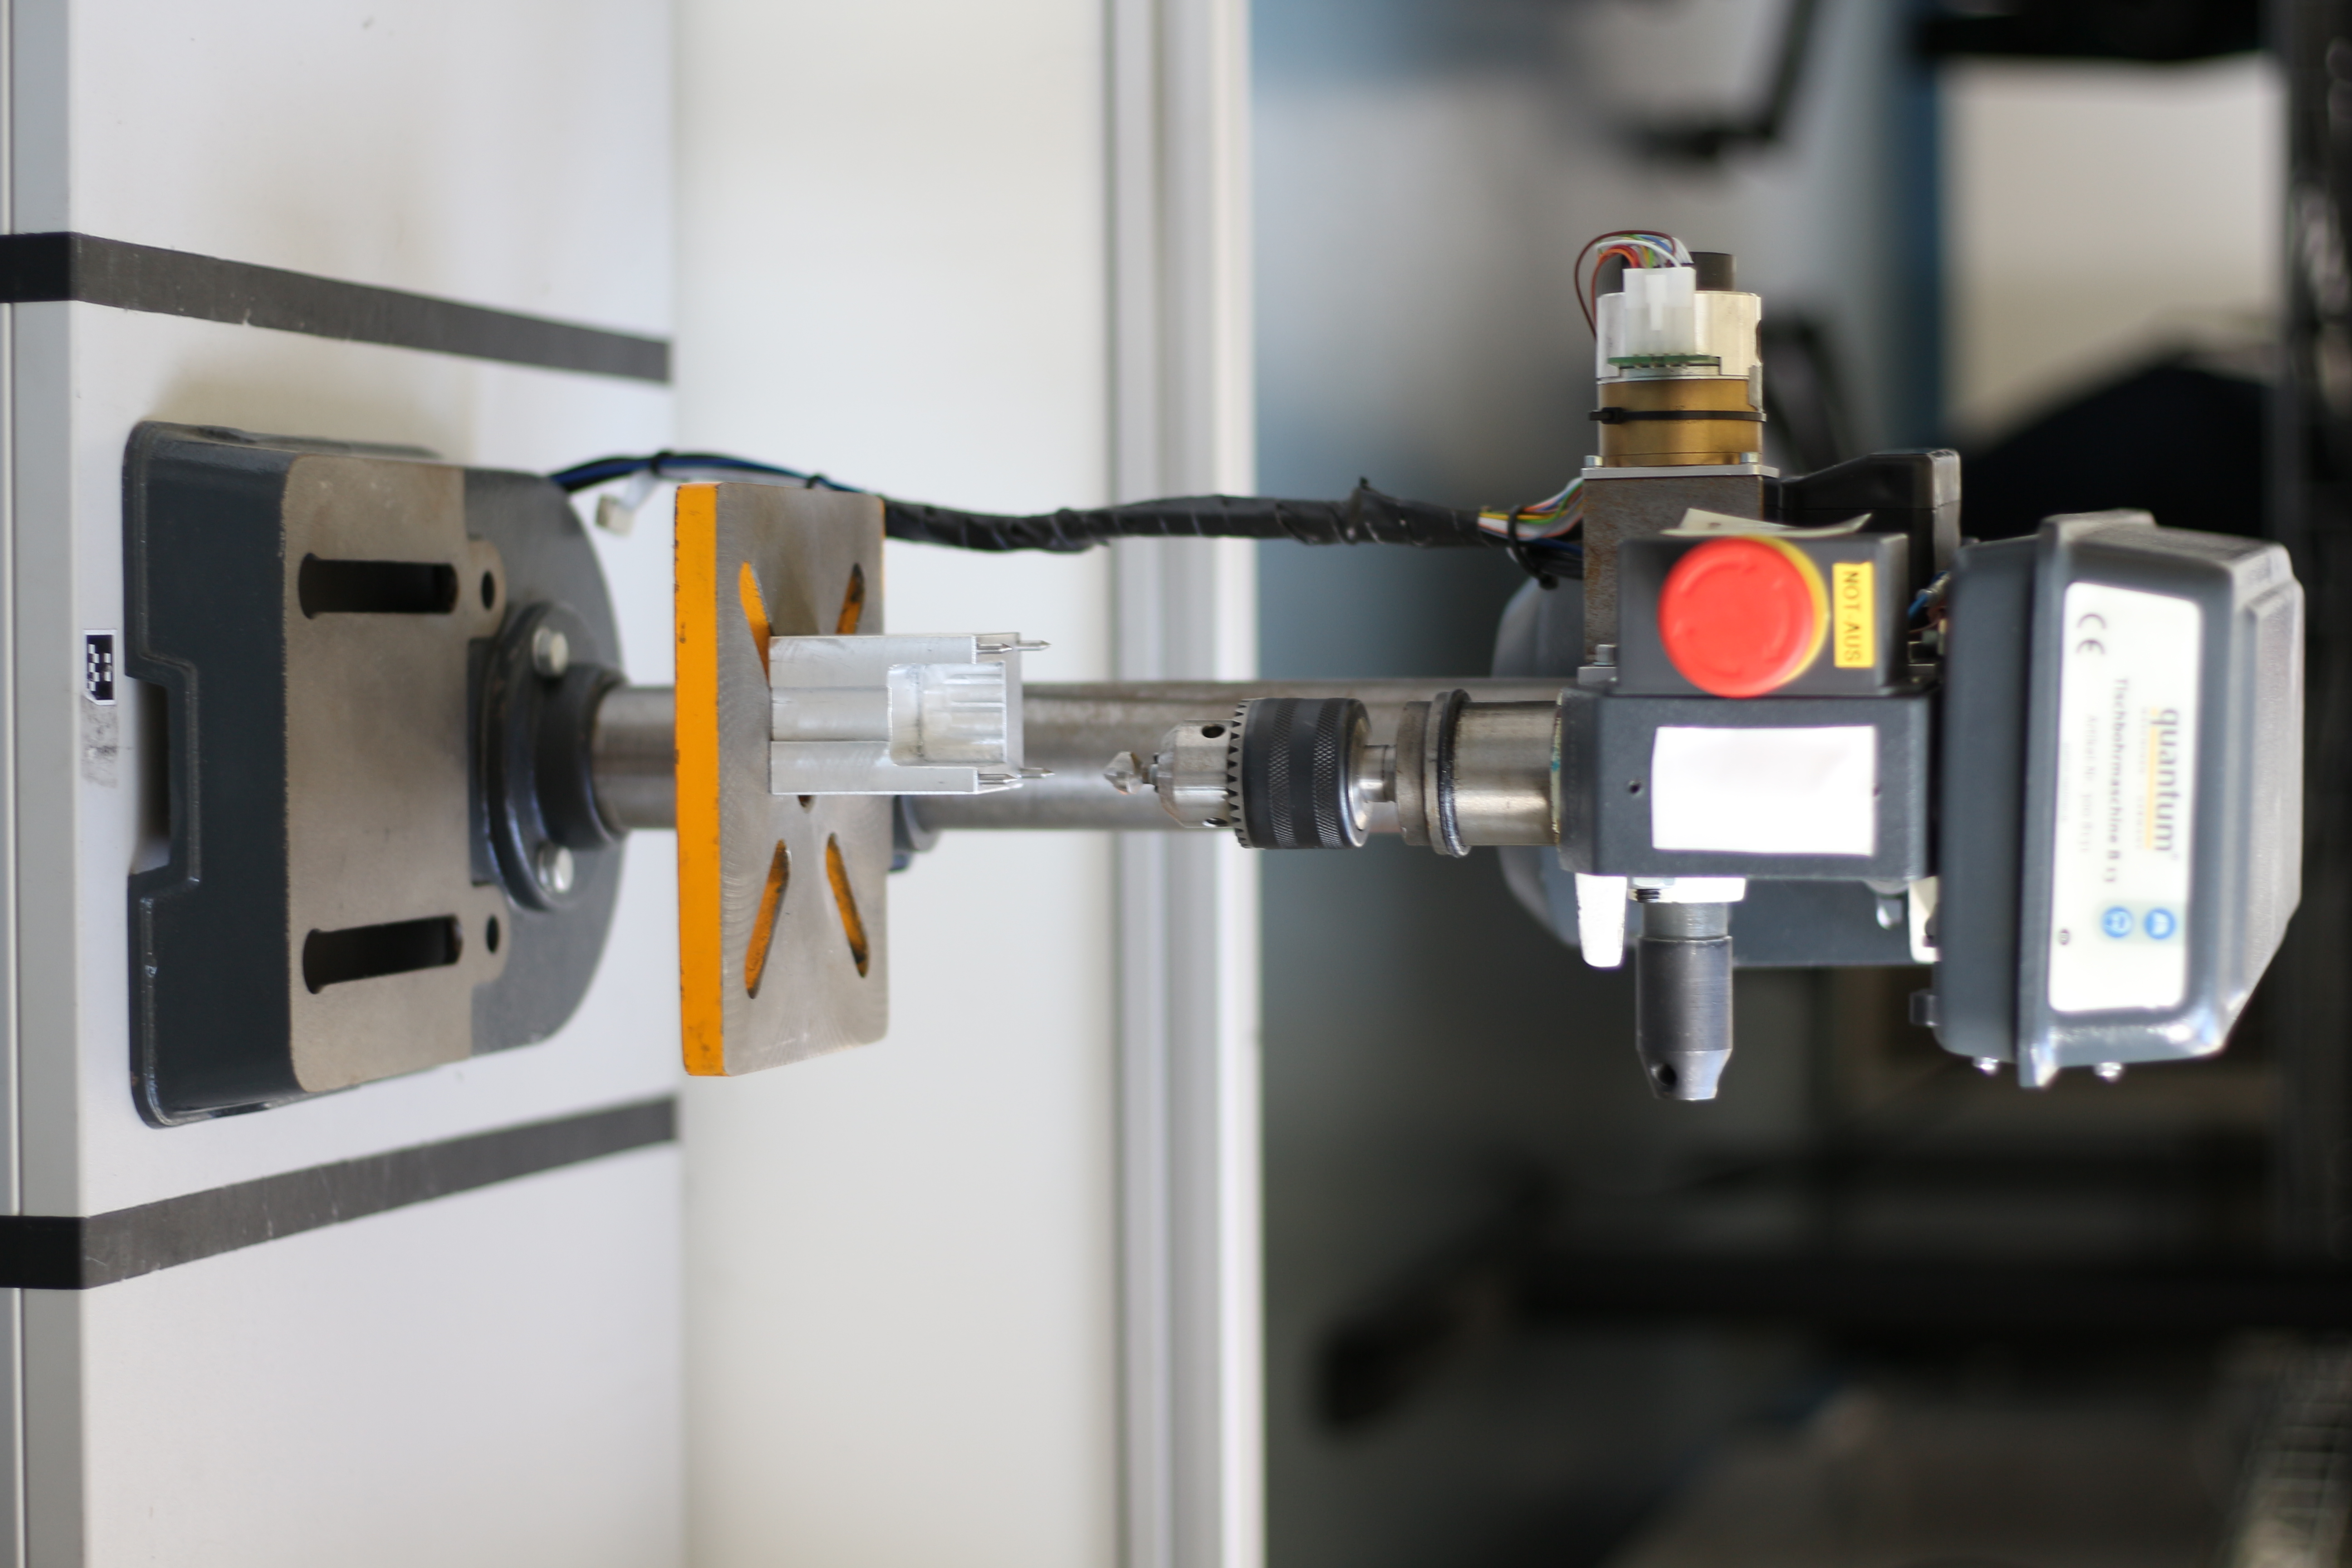
\includegraphics[height=45mm,angle=90,trim=0px 0px 0px 0px,clip]
	  		{pics/atwork/networked_devices/drillingMachine.jpg}
			}
		   \label{fig:coverPlateDrillingMachine}
		}
		\hfill
		 \subfigure[Quality control camera]{
		  \scalebox{1.0}[1.0]{
  		  \includegraphics[height=45mm,angle=90,trim=0px 0px 0px 0px,clip]
	  		{pics/atwork/networked_devices/QCC.jpg}
			}
			\label{fig:coverPlateQCC}
		}
		\hfill\mbox{}
	  \caption{Networked devices for the plate drilling task}
  	\label{fig:plateDrillingNetworkedDevices} 
	\end{center}
\end{figure}


%--------------------------------------------------------------------
\subsubsection{Feature Variation}
\label{sssec:TaskPlateDrillingVariation}


The task can have different variations as shown in the following examples.
\begin{itemize}
 \item The sequence of faulty, unusable and perfect plates flowing through the conveyor belt.
 \item The cover plate orientation on the conveyor belt.
 \item The number of plates delivered in each category (faulty, unusable and perfect).
\end{itemize}
Furthermore, the solutions can vary depending on the sequence of activities being performed by the robot. The robot can choose to:

\begin{itemize}
	\item collect all cover plates from the conveyor belt first and process them collectively or
	\item perform the task for one cover plate at a time before collecting the next cover plate from the conveyor belt
\end{itemize}


%--------------------------------------------------------------------
\subsubsection{Input Provided}
\label{sssec:TaskPlateDrillingInput}
The team will be provided with the following information:
\begin{itemize}
\item 3D CAD textured models of the plates
\item Description of three different states of the plate (faulty, unusable, perfect). 
The three different states of the cover plate are shown in Figure \ref{fig:coverPlateStates}.
\item Location of objects related to the task.
\end{itemize}

%--------------------------------------------------------------------
\subsubsection{Expected Robot Behavior or Output}
\label{sssec:TaskPlateDrillingOutput}
The robot operates the conveyor belt and receive the incoming cover plates. 
The robot will fix the faulty cover plates with the drilling machine and deliver the unusable cover plates to trash container box.
The robot has the option to receive and process the plates collectively or individually.

\begin{figure}[htb]
  \begin{center}
  	\hfill
	  \subfigure[Trash container box]{
		  \scalebox{1.0}[1.0]{
  		  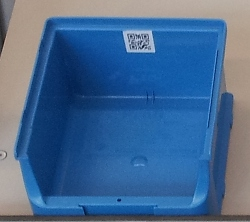
\includegraphics[height=35mm,angle=0,trim=0px 0px 0px 0px,clip]
	  		{./fig/Blue_box.jpg}
			}
		   \label{fig:coverPlateUnusableContainerBox}
		}
		\hfill
		 \subfigure[Cover plate file card box]{
		  \scalebox{1.0}[1.0]{
  		  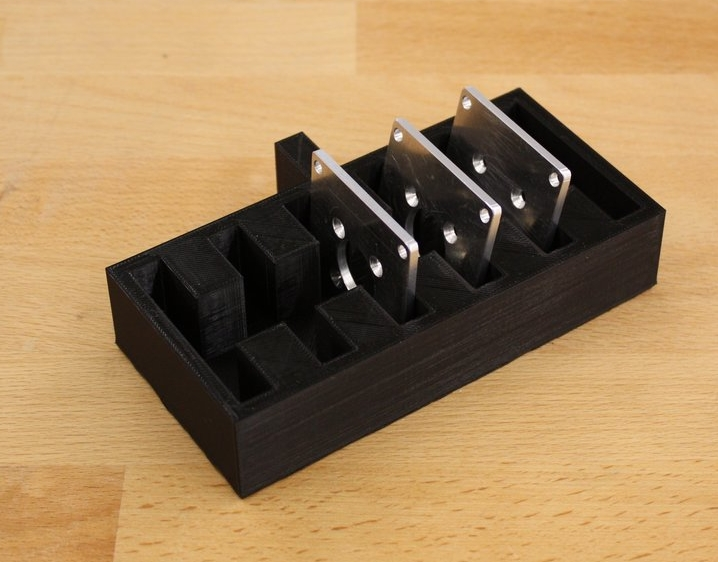
\includegraphics[height=35mm,angle=0,trim=0px 0px 0px 0px,clip]
	  		{pics/atwork/objects/coverPlatesFileBox.jpg}
			}
			\label{fig:coverPlatesFileBox}
		}%
		\hfill\mbox{}
	  \caption{Designated storage for each cover plate type.}
  	\label{fig:coverPlateStorage} 
	\end{center}
\end{figure}

%--------------------------------------------------------------------
\subsubsection{Procedures and Rules}
\label{sssec:TaskPlateDrillingProcedures}
 \begin{description}
     \item [Step 1] The robot commands the TCB to provide a cover plate in the conveyor belt's exit ramp and waits for the result of the plate recognition from CFH.
     \item [Step 2] The robot should pick up the cover plate and either:
	     \begin{itemize}
	     	\item proceed with processing the cover plate received as described in [Step 3] or
	     	\item request for another cover plate as described in [Step 1]
	     	\end{itemize}
     \item [Step 3] There are two possible sequence of actions that need to be executed by the robot depending on the type of the cover plate. If the cover plate is faulty, the robot needs to deliver this to the trash container box. If the cover plate is unusable, the robot needs to:
     	\begin{itemize}
     		\item place the cover plate inside the drilling machine
     		\item perform correction of the cover plate with the drilling machine
     		\item place the corrected cover plate in the file card box.
     	\end{itemize}
\end{description} 

\subsubsection{Communication with CFH}
\label{sssec:CommCFHPlateDrilling}

The communication and interaction between the robot and the networked device is as follows:

\begin{itemize}
	\item \textbf{Triggered conveyor belt} or \textbf{TCB}. This TCB is a composite of the quality control camera and the conveyor belt. The operation of the TCB involves the message types TriggeredConveyorBeltCommand \cite{rockin:CFHMessages}, TriggeredConveyorBeltStatus \cite{rockin:CFHMessages} and Inventory \cite{rockin:CFHMessages}.
For each TriggeredConveyorBeltCommand::START command and \emph{next cycle id} received, the TCB will run the conveyor belt until a cover plate has been recognized and placed in the conveyor belt exit ramp and stop the belt again. 

The \emph{next cycle id} is used to determine the cycle for which the command is executed. It must be exactly one greater than the cycle received via the TriggeredConveyorBeltStatus (next\_cycle = cycle + 1). The cycle determines how often the TCB has already been activated. Every time that the TCB is commanded by a robot, the cycle counter is increased.

The TCB provides information on the type of cover plate (\emph{faulty} or \emph{unusable}) by updating the inventory of the CFH.
	\item \textbf{Drilling machine}. The operation of the drilling machine involves message type DrillingMachineCommand \cite{rockin:CFHMessages} and DrillingMachineStatus \cite{rockin:CFHMessages}
	The drill of the drilling machine will spin continuously and the robot needs to command the drill to move down and up (message of type DrillingMachineCommand \cite{rockin:CFHMessages}). 
	In order to move down the drill, the variable command needs to be set to Command::MOVE\_DOWN. 
	To move the drill up again the variable needs to be set to Command::MOVE\_UP.
	An example in C++ is provided \cite{rockin:CFHExamples}. 
	Additionally, the CFH sends a status message of type DrillingMachineStatus \cite{rockin:CFHMessages} indicating whether the drill is at the top position (state is equal to State::AT\_TOP), at the bottom position (state is equal to State::AT\_BOTTOM), moving down (state is equal to State::MOVING\_DOWN) or moving up (state is equal to State::MOVING\_UP). In case of a problem, the state is equal to State::UNKNOWN.
\end{itemize}

%--------------------------------------------------------------------
\subsubsection{Acquisition of Benchmarking Data}
\label{sssec:TaskPlateDrillingData}

General information on the acquisition of benchmarking data is described in Section \ref{sec:TbmAcquisitionOfData}.

\paragraph{Online Data} In order to send online benchmarking data to the CFH, the robot has to use the \textbf{BenchmarkFeedback} message. The message contains:
\begin{itemize}
	\item after\_receiving (type: PlateState) 
	\item after\_drilling (type: PlateState) 
\end{itemize}

The \textbf{BenchmarkFeedback} message can be found at \cite{rockin:CFHMessages}.

\paragraph{Offline data} 
The additional information described in the following table has to be logged:

\begin{table}[h]
	\centering
	\begin{footnotesize}
		\begin{tabular}{|l|l|l|l|}
			\hline
			Topic	&	Type		&	Frame Id		&	Notes \\ \hline\hline
			/rockin/drill\_command\tablefootnote{Drilling commands issued by the robot} & std\_msgs/Int32 & -- & when issued \\ \hline
			/rockin/qcc\_command\tablefootnote{QCC commands issued by the robot} & std\_msgs/Int32 & -- & when issued \\ \hline
			/rockin/plate\_condition\tablefootnote{Condition of each plate, as evaluated by the robot, after drilling} & std\_msgs/Int32 & -- & when issued \\ \hline
		\end{tabular}
	\end{footnotesize}
\end{table}

%--------------------------------------------------------------------
\subsubsection{Scoring and Ranking}
\label{sssec:TaskPlateDrillingScoring}

Evaluation of the performance of a robot according to this task benchmark is based on performance equivalence classes. Classes are defined in dependence to:
\begin{enumerate}
\item the number and percentage of correctly processed faulty cover plates;
\item the number and percentage of correctly processed unusable cover plates;
\item execution time (if less than the maximum allowed for the benchmark).
\end{enumerate}

\noindent 
\paragraph{Achievements} The set $A$ of achievements for this task includes:
\begin{itemize}
\item the robot communicates with the CFH throughout the test;
\item the team submits the benchmarking data appropriately by the end of the test;
\item the robot picks up a cover plate from the conveyor belt's exit ramp;
\item the robot places an unusable cover plate into the trash container box;
\item the robot completely processes an unusable cover plate (pick up an unusable cover plate from the exit ramp of the conveyor belt and place it into the trash container box);
\item the robot places a faulty cover plates inside the drilling machine;
\item the robot performs the drilling of a faulty cover plate using the drilling machine;
\item the robot completely corrects a faulty cover plate (pick up a faulty cover plate from the exit ramp of the conveyor belt, place it inside the drilling machine and operate the drilling machine);
\item the robot picks up a corrected cover plate from the drilling machine;
\item the robot places a corrected cover plate into the file card box;
\item the robot completely delivers a corrected cover plate (pick up a corrected cover plate from the drilling machine and place it inside the file card box).
\end{itemize}

%--------------------------------------------------------------------
% EOF
%--------------------------------------------------------------------

%!TEX root = ./ERL Industrial Robots.tex


%--------------------------------------------------------------------
%--------------------------------------------------------------------
\subsection{Task \emph{Fill a Box with Parts for Manual Assembly (Shared with RoboCup@Work)}}
\label{ssec:TaskFillaBox}

This task reflects one of the primary requisites of a mobile robotic service assistant, i.e., to work together with humans. In this case the goal is to assist humans at a manual assembly workstation.
The robots have to deal with flexible task specifications, especially concerning information about object constellations in source and target locations, and task constraints such as limits on the number of objects allowed to be carried simultaneously, etc. 

%--------------------------------------------------------------------
\subsubsection{Task Description}
\label{sssec:TaskFillaBoxDescription}

The robot has to pick up several parts from different source locations and deliver them to several destination locations. 
%\begin{figure}[!htbp]
%	\begin{center}
%		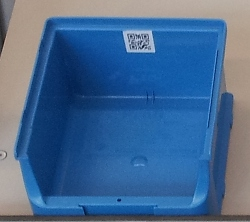
\includegraphics[scale=0.5,angle=0]{fig/Blue_box}
%		\caption{\erlir container with identifier}
%		\label{fig:AidTrayRack2}
%	\end{center}
%\end{figure}

%--------------------------------------------------------------------
\subsubsection{Feature Variation}
\label{sssec:TaskFillaBoxVariation}

%The standardized boxes (see Figure \ref{fig:AidTrayRack2}) can be used for several groups of parts. Because of variations in containing parts (e.g., bearing box variations) the groups of parts in this task vary the same way. 
All objects defined in Section \ref{sssec:PartstoManipulate} will be used in this task.
Several containers (see Section \ref{sssec:EnvironmentObjectstoRecognize}) can be present in the environment and are always associated with a workstation or shelf. It is possible that more than one container is placed on top of a single workstation. Currently, a container itself does to not need to be manipulated or transported by the robot.

For any major competition in which \erlir will be present, additional objects may be used.
Those objects can be found in the rule descriptions of the major competition (e.g. for RoboCup 2016)
%--------------------------------------------------------------------
\subsubsection{Input Provided}
\label{sssec:TaskFillaBoxInput}

The team will be provided with the following information:
%
\begin{itemize}
\item The list of possible parts used in the task;
\item The list of source service areas
\item The list of destination service areas
\end{itemize}

%--------------------------------------------------------------------
\subsubsection{Expected Robot Behavior or Output}
\label{sssec:TaskFillaBoxOutput}

The task execution is triggered by the robot receiving the inventory- and order list from the CFH.
The robot proceeds with collecting the parts from the source locations and transports them to the destination service areas.

%--------------------------------------------------------------------
\subsubsection{Procedures and Rules}
\label{sssec:TaskFillaBoxProcedures}

 There can be multiple obstacles and barrier tapes (color: yellow/black) present in the environment that might block the direct path of the competing robot. The robot must avoid all obstacles or even other robots during the execution of the complete task.
%
\begin{description}
\item[Step 1] The robot will receive an order and inventory from the CFH containing a list of objects to be collected and delivered.
\item[Step 2] The robot must plan the best path to the designated workstation, passing through each storage area where the required objects for a requested product in the list can be found. 
\item[Step 3] The robot must execute the above path, collect the objects and then deliver them to the designated destination locations.
\item[Step 4] The Steps 2 and 3 above must be done for all the objects in the list mentioned above in Step 1.
\end{description}

%--------------------------------------------------------------------
\subsubsection{Communication with CFH}
\label{sssec:CommCFHFillaBox}

For this task benchmark the robot does not have to control any networked device in the environment. Thus, the robot is only supposed to receive the static inventory and order information once. Currently, the robot does not need to update the inventory information.

%--------------------------------------------------------------------
\subsubsection{Acquisition of Benchmarking Data}
\label{sssec:TaskFillaBoxData}
General information on the acquisition of benchmarking data is described in Section \ref{sec:TbmAcquisitionOfData}.

\paragraph{Online Data}
\begin{itemize}
\item No online benchmarking data has to be sent to the CFH during this task benchmark.
\end{itemize}

\paragraph{Offline data} 
The additional information described in the following table has to be logged:
\begin{table}[h]
	\centering
	\begin{footnotesize}
		\begin{tabular}{|l|l|l|l|}
			\hline
			Topic	&	Type		&	Frame Id		&	Notes \\ \hline\hline
			/rockin/notification\tablefootnote{The string with the notification of the perceived object should be in a tab separated string: CLASS OBJECT\_ID X Y THETA} & std\_msgs/String & -- & -- \\ \hline
		\end{tabular}
	\end{footnotesize}
\end{table}

%--------------------------------------------------------------------
\subsubsection{Scoring and Ranking}
\label{sssec:TaskFillaBoxScoring}

Evaluation of the performance of a robot according to this task benchmark is based on performance equivalence classes. Classes are defined in dependence to the number of parts of the product to be assembled actually provided by the robot to the human worker and their order according to the desired one.

%\noindent%
\paragraph{Achievements} The set $A$ of achievements for this task consists of:
%
\begin{itemize}
\item The robot communicates with the CFH throughout the test;
\item The team submits the benchmarking data by the end of the test;
\item The robot picks up a required object from its storage location;
\item The robot places the required objects in its destination area;
\item The robot has correctly collected and delivered all objects
\end{itemize}
%--------------------------------------------------------------------
% EOF
%--------------------------------------------------------------------

%\newpage
\section{Basic Transportation Test}

\paragraph{Purpose and Focus of the Test}
The purpose of this TBM is to assess the ability of the robots for combined navigation and manipulation tasks. 
The robots have to deal with flexible task specifications, especially concerning information about object constellations in source and target locations, and task constraints such as limits on the number of objects allowed to be carried simultaneously, etc.  

\paragraph{Scenario Environment}
The arena used for this test contains all elements as for the Basic Manipulation Test. Besides that all areas may contain objects.

\paragraph{Manipulation Objects}
The manipulation objects used in this test are defined by the instances described in Table~\ref{ssec:Objects}.

\paragraph{Task}
A single robot is used, which is initially positioned outside of the arena near a gate to the arena. The task is to get several objects from the source service areas (such as \texttt{S1}, \texttt{T7}, or \texttt{U3}), and to deliver them to the destination service areas (e.g. \texttt{D1} and \texttt{D3}). Robots may carry up to three objects simultaneously. 
\par
The task specification consists of two lists:
The first list contains for each service area a list of manipulation object descriptions. The descriptions are similar as those used for the Basic Manipulation Test. 
The second list contains for each destination service area a configuration of manipulation objects the robot is supposed to achieve. The configuration specification is similar as used in the Basic Manipulation Test. 

The term “line” in the task specification can be ignored.

%
%\subsection{Complexity Options}
%The same complexity scoring as in BMT applies.

\paragraph{Rules}
The following rules have to be obeyed:

\begin{itemize}
\item The order in which the teams have to perform will be determined by a draw.
\item The robot has to start from outside the arena.
\item The robot will get the task specification from the referee box.
\item After the team's robot starts, it must move into the arena and attempt to complete the task. 
\item A manipulation object counts as successfully grasped as specified in Section~\ref{ssec:GraspingObjects}.
\item A manipulation object counts as successfully placed, if the robot has placed the object into the correct destination service area as described in Section~\ref{ssec:PlacingObjects}.
\item It is not allowed to place manipulation objects anywhere except for the robot itself and any of the available service areas.
\item A robot may carry up to three objects at the same time.
\item The time is stopped when the robot has completed the task (delivered all objects to the right locations and left the arena through the exit gates). If a team cannot complete the task within the designated time, the run will be stopped.. 

\end{itemize}


%
%\subsection{Scoring}
%Points are awarded as follows:
%
%\begin{itemize}
%\item 75 points are awarded for successfully grasping a manipulation object required in the task specification.. 
%\item - 75 points if a wrong object has been grasped
%\item 75 points are awarded for successfully placing a manipulation object into the destination service area.
%\item 50 points are awarded for completing the task specification completely correct. 
%\item The reached points of a test will be multiplied with a defined complexity factor depending on the previously chosen complexity level
%\end{itemize}
%



%--------------------------------------------------------------------
%--------------------------------------------------------------------
%--------------------------------------------------------------------
\clearpage
\section{Functionality Benchmarks}
\label{sec:FunctionalityBenchmarks}

\paragraph{Communication with CFH}
\label{ssec:CommCFH}
Every functionality benchmark will be preceded by a safety-check similar to that described for the task benchmark procedures.
All teams are required to perform each functionality benchmark according to the steps mentioned in their respective section. During the competition, all teams are required to repeat it the functionality benchmark several times. On the last day, only a selected number of top teams will be allowed to perform it.


%!TEX root = ./ERL Industrial Robots.tex

%--------------------------------------------------------------------
%--------------------------------------------------------------------
\subsection{Object Detection Functionality}
\label{ssec:ObjectPerception}

%--------------------------------------------------------------------
\subsubsection{Functionality Description}
\label{sssec:ObjectPerceptionDescription}

This functionality benchmark evaluates robot capabilities of locating an object at a given location. One of the common tasks for service and industrial robots is to locate the object which can possibly be placed at a particular location. 
In addition to that, several secondary objects and decoys may be present at the location too. 
The robot is required to find particular objects among a set of objects and decoys. 
The target object is either included or not depending on the variation for every trial.

Objects presented to the robot in this functionality benchmark are based on the the \erlir factory scenario.
Teams are provided with a list of objects (object instances), subdivided into classes (see Section \ref{sssec:ObjectPerceptionInput}).
The objects that are used here are described in Section~\ref{sec:TestBed}.
%In this benchmark, the robot is expected to detect and estimate the object's class and identity.

%--------------------------------------------------------------------
\subsubsection{Feature Variation}
\label{sssec:ObjectPerceptionVariation}

%For this benchmark, the variation space for object features is represented by the (known) set of objects that the robot may be presented with.
For this benchmark, the variation space for objects includes: 1. A set of objects and decoys and their poses; 2. The presence of the target object [yes, no].
Furthermore, the variation space for object location is the surface of the benchmarking area where objects are located (see Section \ref{sssec:ObjectPerceptionInput}).

%--------------------------------------------------------------------
\subsubsection{Input Provided}
\label{sssec:ObjectPerceptionInput}

The set of individual objects that will actually be presented to the robot during the execution of the functionality benchmark is described in Section \ref{ssec:Objects}. 
%Object instances are subdivided into classes of objects that have one or more properties in common (``object classes''). 
%Objects of the same class share one or more properties, not necessarily related to their geometry (for instance, a class may include objects that share their application domain). 
Each object class is assigned a unique ID.

The team does not know which object instances will actually be presented to the robot during the benchmark. 
However, the team will be provided with the object information described in Section \ref{ssec:Objects}.
%
%\begin{itemize}
%\item Descriptions/models of all the object classes in the form of 3D textured models;
%\item Object classes such as Motor, KitkatMini, etc.
%\end{itemize}

Object descriptions will be expressed according to widely accepted representations, well in advance of the competition. 

%--------------------------------------------------------------------
%\subsubsection{Expected Robot Behavior or Output}
%\label{sssec:ObjectPerceptionOutput}
%
%The robot, for a set of several objects presented to it, must locate the target object. 

%\begin{itemize}
%\item Object detection: perception of the presence of an object on the table and association between the perceived object and one of the object classes (see Section \ref{sssec:ObjectPerceptionInput}).
%\item Object recognition: association between the perceived object and one of the object instances belonging to the selected class (see Section \ref{sssec:ObjectPerceptionInput}).
%
%\end{itemize}
%The following list of classes and instances of objects are going to be used in the object perception functionality benchmark:
%\begin{itemize}
%    \item Industrial
%
%    \item Chocolates
%
%    \item T-LESS
%
%\end{itemize}

%--------------------------------------------------------------------
\subsubsection{Procedures and Rules}
\label{sssec:ObjectPerceptionProcedures}

The maximum time allowed for one functionality run is 20 seconds. The time starts when the robot sends the start message to CHF until the robot sends the result message. A timeout is recorded for that run if it exceeds the allocated time and the robot must prepare for the next run.

\begin{description}
\item[Step 1] A set of target and secondary objects, decoys will be placed in front of the robot. The setup is fixed for all teams.
\item[Step 2] The robot must locate the target object represented in one of two ways:
	\begin{itemize}
	\item The 3D bounding box of the robot with respect to the robot base. In this case, the robot must provide a point cloud of the scene (transformed to the robot's base frame) corresponding to the 3D bounding box.
	\item The 2D bounding box of the objects in an image. The robot must provide the raw RGB image of the scene corresponding the 2D bounding box.
	\end{itemize}
\item[Step 3] The preceding steps are repeated until 10 runs have been completed.
\end{description}

%--------------------------------------------------------------------
\subsubsection{Communication with CFH}
\label{sssec:CommCFHObjectPerception}
For this functionality benchmark the robot does not have to control any networked device in the environment. Only the communication as described below is necessary:

\begin{description}
\item[Step 1] The robot sends a \textbf{BeaconSignal} message at least every second.
\item[Step 2] The robot waits for a \textbf{BenchmarkState} message. It starts the benchmark execution when the \emph{phase} field is equal to EXECUTION and the \emph{state} field is equal to RUNNING.
\item[Step 3] As soon as the robot has finished perceiving the object, it sends a message of type \textbf{BenchmarkFeedback} to the CFH with the required results and the \emph{phase\_to\_terminate} field set to EXECUTION. The robot should do this until the \textbf{BenchmarkState}'s \emph{state} field has changed.
\item[Step 4] The robot continues with Step 2.
\item[Step 5] The functionality benchmark ends when the \textbf{BenchmarkState}'s \emph{state} field is equal to FINISHED.
\end{description}
\noindent
The messages to be sent and to be received can be seen on the Github repository located at \cite{rockin:CFHMessages}.

%--------------------------------------------------------------------
\subsubsection{Acquisition of Benchmarking Data}
\label{sssec:ObjectPerceptionData}

Each team has to locally record the following data (at minimum):
\begin{itemize}
	\item RGB camera stream of the robot
	\item Point cloud of the scene if 3D bounding box is provided
	\item Raw RGB image if 2D bounding box is provided
\end{itemize}

The teams are encouraged to provide the dataset used for training the model.

%--------------------------------------------------------------------
\subsubsection{Scoring and Ranking}
\label{sssec:ObjectPerceptionScoring}

We use the metrics, illustrated in figure \ref{fig:ObjectDetectionMetrics}, to evaluate the performance of the robot:
\begin{itemize}
	\item True Positive (TP): the robot detects the target object when it is present
	\item False Positive (FP): the robot detects wrong object whether the target object is present or not
	\item False Negative (FN): the robot does not detect any object when the target object is present
	\item True Negative (TN): the robot does not detect any object when the target object is not present
\end{itemize} 
\begin{figure}[h!]
	\centering
	\begin{tikzpicture}	
	\node[label={\small TP}, anchor=south west,inner sep=0](B) at (-4,1) {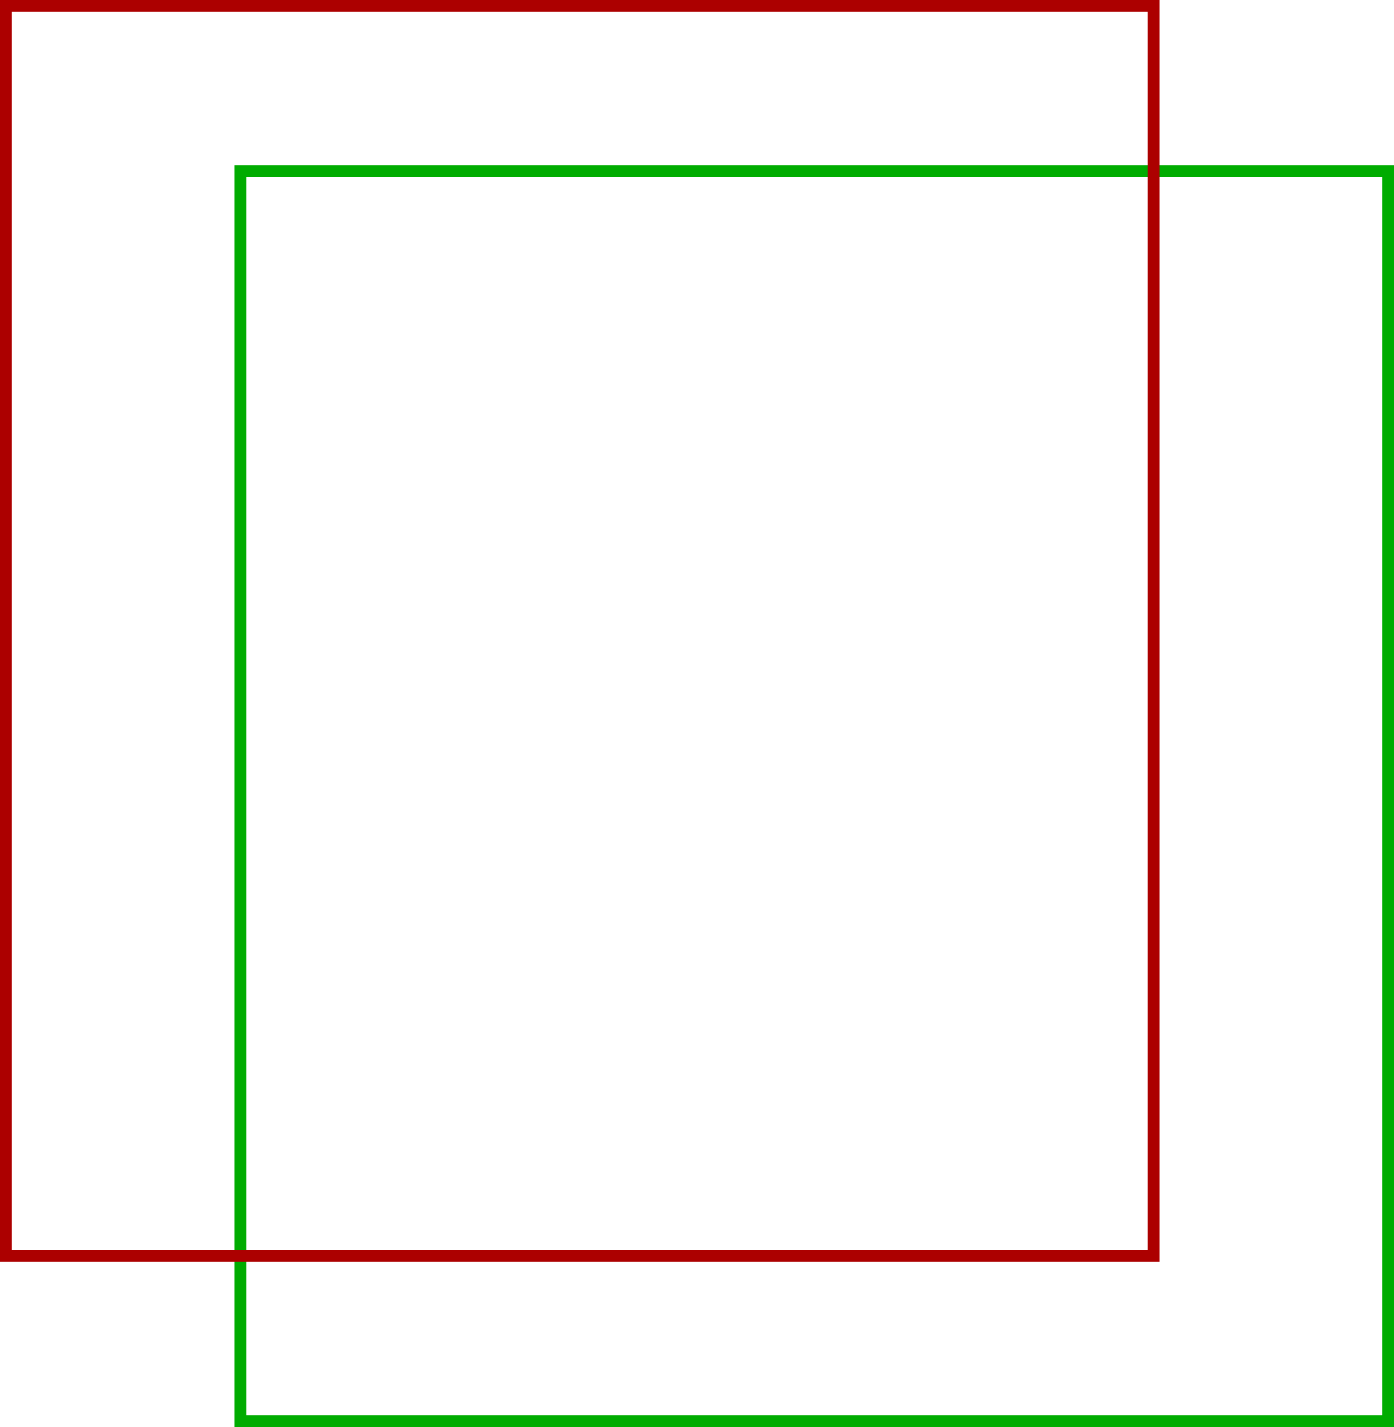
\includegraphics[width=3cm]{fig/FBM/erl/perception/sciroc-op-TP.png}};
	
	\node[label={\small FP},anchor=south west,inner sep=0](D) at (0,0.8) {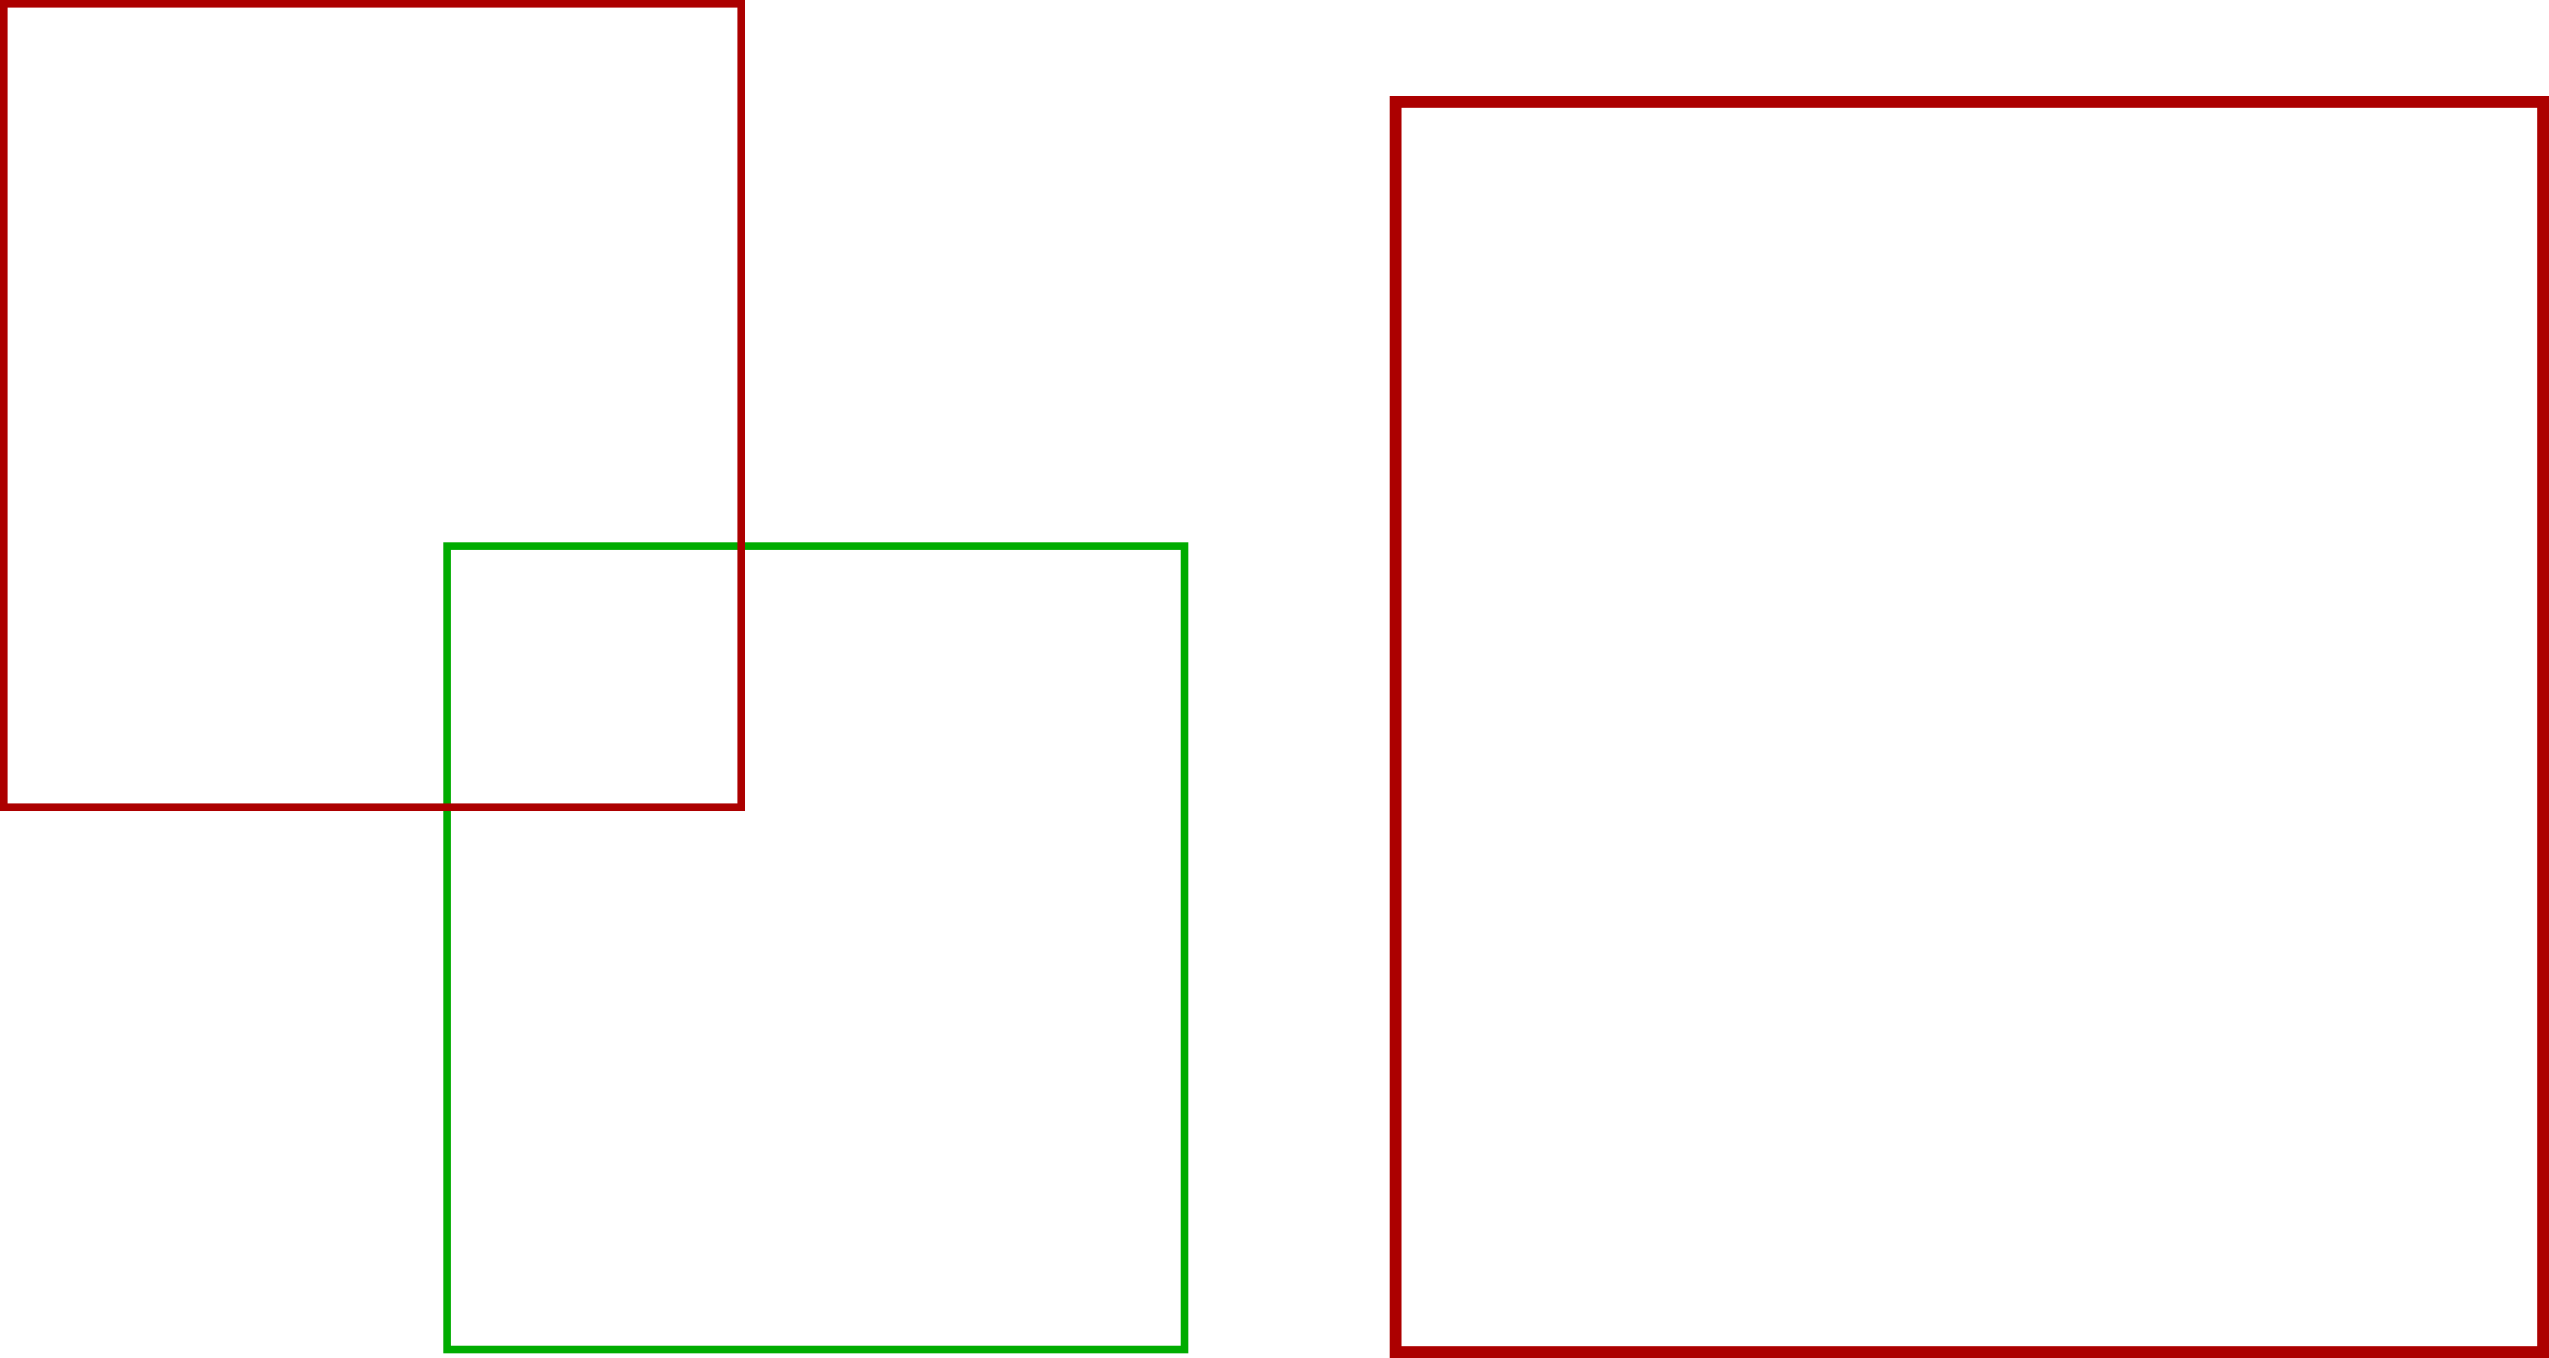
\includegraphics[width=6cm]{fig/FBM/erl/perception/sciroc-op-FP.png}};
	
	\node[label={\small FN}, anchor=south west,inner sep=0](C) at (-3.75,-3.5) {
\includegraphics[width=2.5cm]{fig/FBM/erl/perception/sciroc-op-FN.png}};
	
	\node[label={\small TN},anchor=south west,inner sep=0](E) at (1.75,-3.6) {
\includegraphics[width=2.5cm]{fig/FBM/erl/perception/sciroc-op-TN.png}};
	
	\node[anchor=south west,inner sep=0](E) at (7,3) {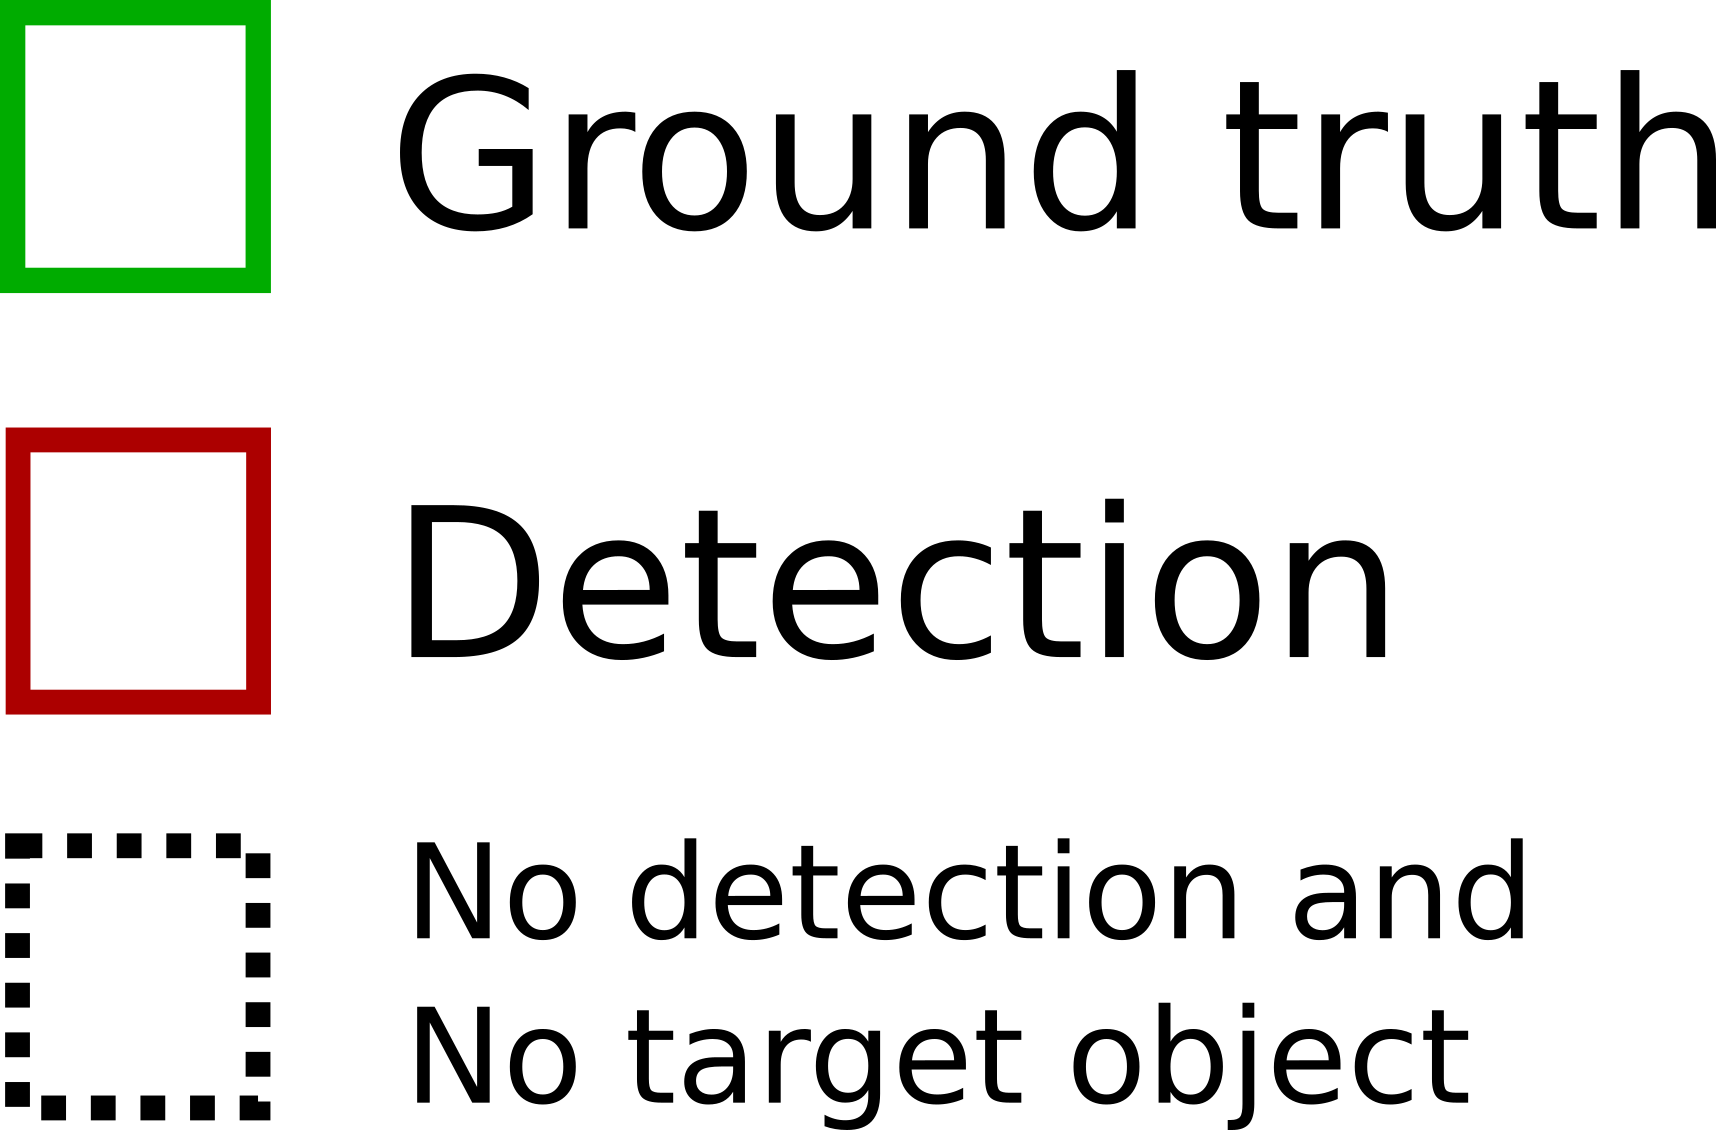
\includegraphics[width=2cm]{fig/FBM/erl/perception/sciroc-op-legend.png}};
	\end{tikzpicture}
	\caption{Metrics for object detection functionality benchmark}
	\label{fig:ObjectDetectionMetrics}
\end{figure}

For the TP and FP, the measurement is based on the degree of similarity between the ground truth and detected bounding boxes. We use the Intersection over Union (IoU),

\begin{equation}
IoU = \frac{B_{GT} \cap B_{DET}}{B_{GT} \cup B_{DET}}
\end{equation}
where $B_{GT}$ and $B_{DET}$ area the ground truth and detected bounding boxes respectively. The intersections are calculated as areas and volumes for 2D and 3D bounding boxes respectively.
In figure \ref{fig:ObjectDetectionSample} the green and red boxes show the ground truth and detected bounding boxes respectively. If the IoU is greater than a given threshold, the detection result is considered to be a true positive and otherwise it is a true negative. The same rule applies to 3D bounding boxes except that the areas will be replaced by volumes.
The IoU threshold is a configurable parameter ranging from 0.5 to 0.95 with a step size of 0.05. This approach is borrowed from the COCO challenge \footnote{https://cocodataset.org/\#detection-eval}. The TP and FP are then averaged over all IoU thresholds.


\begin{figure} [h!]
	\begin{center}
		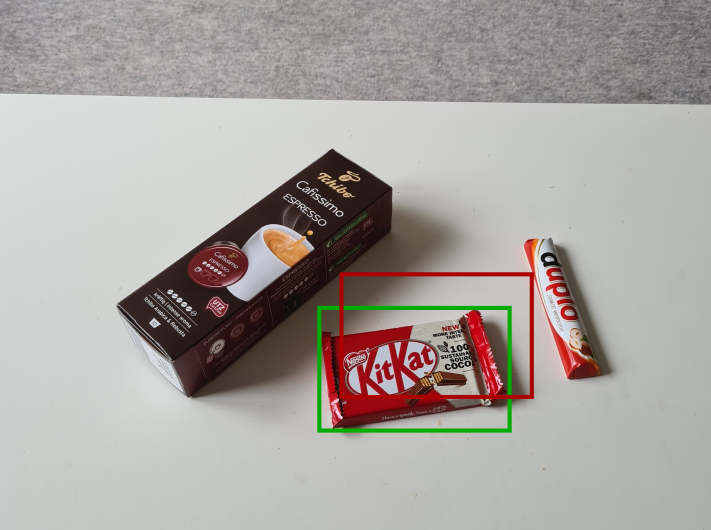
\includegraphics[width=7cm]{fig/FBM/erl/perception/sciroc-op-chocholates-bbox.png}
	\end{center}
	\caption{Object detection example: green bounding box is the ground truth and the red one is the detection.}
	\label{fig:ObjectDetectionSample}
\end{figure}

Evaluation of the performance of a robot according to this functionality benchmark is based on:
%
\begin{enumerate}
\item The sum of the TP and TN;
\item The team with the lower FP count is ranked higher;
\item The team with the lower FN count is ranked higher.
\end{enumerate}
%
The previous criteria are in order of importance; the first criterion is applied first and teams will be scored according to their accuracy, the ties are broken by using the second one still applying accuracy metrics, and in case of ties we will resort to the FN count.


%--------------------------------------------------------------------
% EOF
%--------------------------------------------------------------------

%!TEX root = ./ERL Industrial Robots.tex


%--------------------------------------------------------------------
%--------------------------------------------------------------------
\subsection{Manipulation Pick Functionality}
\label{ssec:Manipulation}

%--------------------------------------------------------------------
\subsubsection{Functionality Description}
\label{sssec:ManipulationDescription}

This functionality benchmark assesses the robot's capability of grasping different objects. 
An object from a known set of possible objects is presented in the test for the robot to be identified and grasped.
After identifying the object, the robot needs to perform the grasping motion, lift the object and notify that the object is acquired.

%--------------------------------------------------------------------
\subsubsection{Feature Variation}
\label{sssec:FBMManipulationVariation}

The objects used in the benchmark will be selected from the list of parts to manipulate as presented in Section \ref{ssec:Objects}.
Additionally, the precise position of the object differs in each test.
%--------------------------------------------------------------------
\subsubsection{Input Provided}
\label{sssec:FBMManipulationInput}

The team will be provided with the following information:
\begin{itemize}
	\item The list of possible objects used in the functionality benchmark.
	\item Possible placement of each object used in the functionality benchmark.
\end{itemize}

%--------------------------------------------------------------------
\subsubsection{Expected Robot Behaviour or Output}
\label{sssec:FBMManipulationOutput}

The robot is placed in front of the test area (a planar surface).
One object will be placed in the test area and 
the robot will identify the object and move its end effector on top of it. 
Afterwards, the robot performs the grasping motion of the object and notifies that the grasping has occurred.
The task is repeated with different objects.



%--------------------------------------------------------------------
\subsubsection{Procedures and Rules}
\label{sssec:FBMManipulationProcedures}

The maximum time allowed for one functionality run is 4 minutes (30 seconds for preparation and 210 seconds for execution). A run consists of (1) a preparation phase where the robot is going to its initial configuration and releases a previously grasp object and (2) an execution phase in which the robot detects, localizes, recognizes and manipulates one object.

\begin{description}
\item[Step 1] An object of unknown class and unknown instance will be placed on a table in front of the robot.
\item[Step 2] The robot must determine the object’s class and its instance within that class.
\item[Step 3] The robot must grasp the object, lift it, and notify that grasping has occurred.
\item[Step 4] The robot must keep the grip for a given time while the referee verifies the correct manipulation of the object.
\item[Step 5] The preceding steps are repeated with five different objects.
\end{description} 

For each presented object, the robot must produce the result consisting of:
\begin{itemize}
    \item object class name [string], e.g. containers.
    \item object instance name [string], e.g. EM-02.
\end{itemize}

\subsubsection{Communication with CFH}
\label{sssec:FBMManipulationCommCFH}

For this functionality benchmark the robot does not have to control any networked device in the environment. Only the communication as described below is necessary:

\begin{description}
\item[Step 1] The robot sends a \textbf{BeaconSignal} message at least every second.
\item[Step 2] The robot waits for a \textbf{BenchmarkState} message. It starts the preparation procedure when the \emph{phase} field is equal to PREPARATION and the \emph{state} field is equal to RUNNING.
\item[Step 3] As soon as the robot finishes the preparation phase, it sends a message of type \textbf{BenchmarkFeedback} to the CFH with the \emph{phase\_to\_terminate} field set to PREPARATION. The robot should do this until the \textbf{BenchmarkState}'s \emph{phase} and \emph{state} fields have changed.
\item[Step 4] The robot waits for a \textbf{BenchmarkState} message. It starts the benchmark execution when the \emph{phase} field is equal to EXECUTION and the \emph{state} field is equal to RUNNING.
\item[Step 5] As soon as the robot has finished manipulating the object, it sends a message of type \textbf{BenchmarkFeedback} to the CFH with the required results and the \emph{phase\_to\_terminate} field set to EXECUTION. The robot should do this until the \textbf{BenchmarkState}'s \emph{phase} and \emph{state} fields have changed.
\item[Step 6] The robot continues with Step 2.
\item[Step 7] The functionality benchmark ends when the \textbf{BenchmarkState}'s \emph{phase} field is equal to EXECUTION  and the \emph{state} field is equal to FINISHED.

\end{description}
\noindent
The messages to be sent and to be received can be seen on the Github repository located at \cite{rockin:CFHMessages}.


%--------------------------------------------------------------------
\subsubsection{Acquisition of Benchmarking Data}
\label{sssec:FBMManipulationData}

General information on the acquisition of benchmarking data is described in Section \ref{sec:TbmAcquisitionOfData}. There, the \textbf{offline} part of the benchmarking data can be found.
%
\paragraph{Online data}
In order to send online benchmarking data to the CFH, the robot has to use the \textbf{BenchmarkFeedback} message. The message contains:

\begin{itemize}
	\item grasp\_notification (type: bool)
	\item object\_class\_name (type: string)
	\item object\_instance\_name (type: string)
\end{itemize}

The \textbf{BenchmarkFeedback} message can be found at \cite{rockin:CFHMessages}.

\paragraph{Offline data} 
The additional information described in the following table has to be logged:
\begin{table}[h]
	\centering
	\begin{footnotesize}
		\begin{tabular}{|l|l|l|l|}
			\hline
			Topic				 					&	Type		&	Frame Id		&	Notes \\ \hline\hline
			/rockin/grasping\_pose\tablefootnote{Pose of the grasping position on the object.} 	& geometry\_msgs/PoseStamped & /base\_link & 10 Hz \\ \hline
			/rockin/gripper\_pose\tablefootnote{Pose of the gripper.}	& geometry\_msgs/PoseStamped & /base\_link & 10 Hz \\ \hline
			/rockin/arm\_joints\tablefootnote{Joints data}	& geometry\_msgs/JointState & /base\_link & 10 Hz \\ \hline
		\end{tabular}
	\end{footnotesize}
\end{table}

%--------------------------------------------------------------------
\subsubsection{Scoring and Ranking}
\label{sssec:FBMManipulationScoring}

Evaluation of the performance of a robot according to this functionality benchmark is based on:
%
\begin{enumerate}
\item Number and percentage of correctly identified objects;
\item Number and percentage of correctly grasped objects (the object stops touching the table, see definition below);
\item Execution time (if less than the maximum allowed for the benchmark).
\end{enumerate}
The scoring of teams is based on the number of objects correctly grasped. 
A correct grasp is defined as the object being lifted from the table so to be possible for the judge to pass a hand below it. 
For a grasping to be ``correct'' the position has to be kept for at least 5 seconds from the time the judge has passes the hand below the object. 
The time the judge will require to verify the lifting of the object might be up to 10 seconds. 
In case of ties the overall execution time will be taken into account.

%--------------------------------------------------------------------
% EOF
%--------------------------------------------------------------------

%!TEX root = ./ERL Industrial Robots.tex


%--------------------------------------------------------------------
%--------------------------------------------------------------------
\subsection{Manipulation Place Functionality}
\label{ssec:ManipulationPlace}

%--------------------------------------------------------------------
\subsubsection{Functionality Description}
\label{sssec:ManipulationPlaceDescription}

This functionality benchmark assesses the robot's capability of placing different objects. 
An object from a known set of possible objects is presented in the test for the robot to be placed.
After grasping the object, the robot needs to perform the placing motion, lift the object and place the object in a particular container/box.


\begin{figure}[htb]
	\begin{center}
	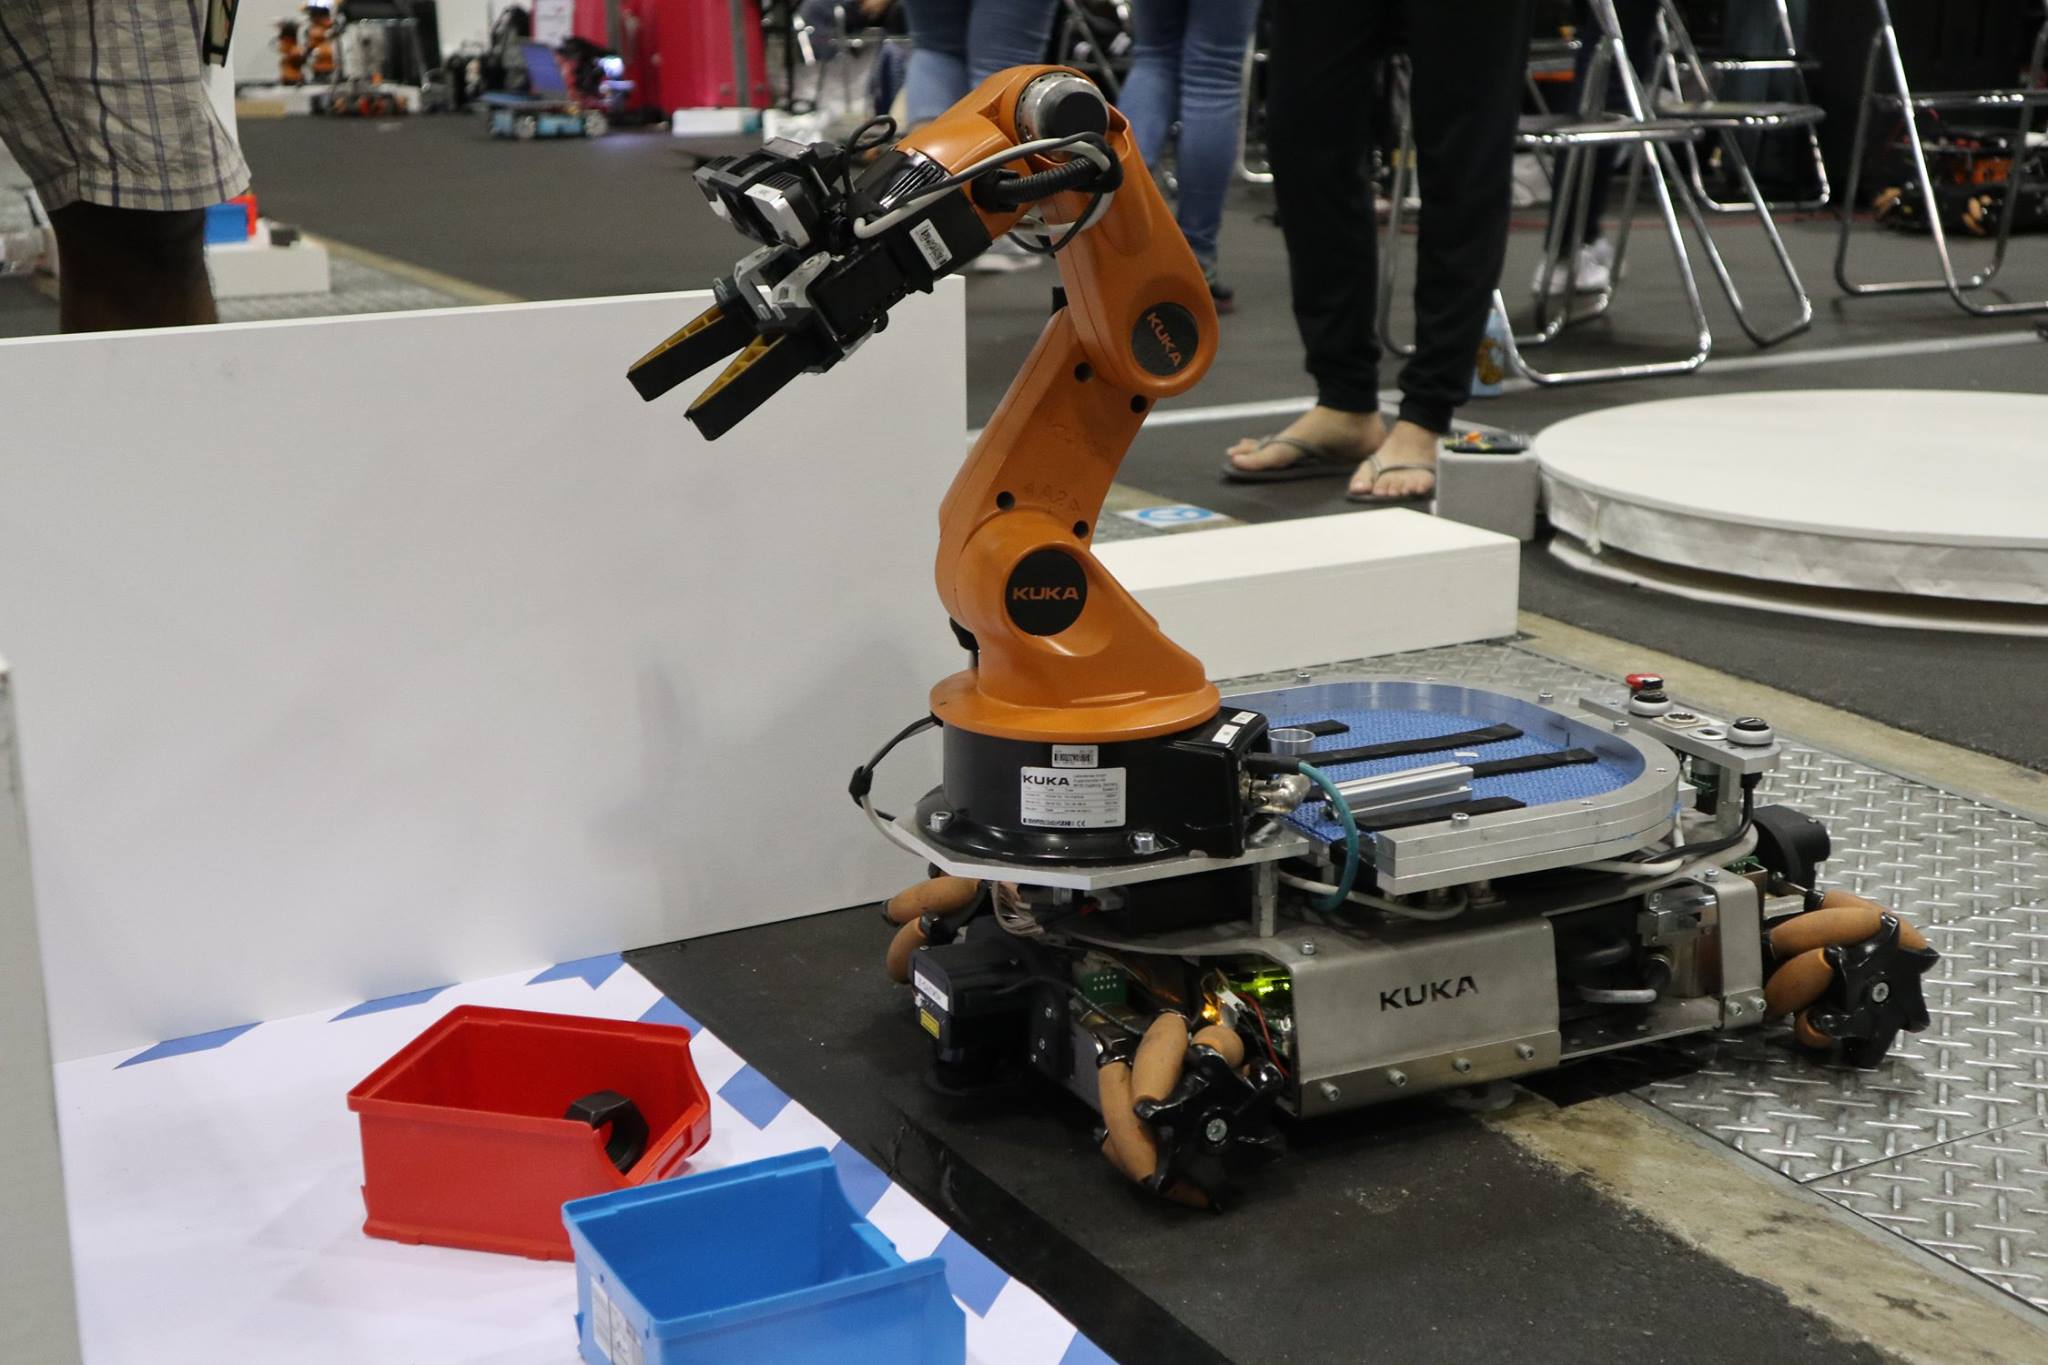
\includegraphics[width=0.45\textwidth]{./fig/FBM/atwork/place_object.jpg}
			\label{fig:MarkerSetEndEffectorWithFrame}
	\caption{Manipulation Place Functionality.}
		\label{fig:ManipulationPlace} 
	\end{center}
\end{figure}
%--------------------------------------------------------------------
\subsubsection{Feature Variation}
\label{sssec:FBMManipulationPlaceVariation}

The objects used in the benchmark will be selected from the list of parts to manipulate as presented in Section \ref{ssec:Objects}.
Additionally, the precise position of the object placement differes in each test.
%--------------------------------------------------------------------
\subsubsection{Input Provided}
\label{sssec:FBMManipulationPlaceInput}

The team will be provided with the following information:
\begin{itemize}
	\item The list of possible objects used in the functionality benchmark.
	\item Possible placement of each object used in the functionality benchmark.
\end{itemize}

%--------------------------------------------------------------------
\subsubsection{Expected Robot Behaviour or Output}
\label{sssec:FBMManipulationPlaceOutput}

The robot is placed in front of the test area (a planar surface).
One object will be placed on the robot or in its gripper.
The robot now has to look the test area for any container to be placed.
The robot performs the placing motion of the object and places the object in particular container in front of it.
After placement it notifies the CFH.



%--------------------------------------------------------------------
\subsubsection{Procedures and Rules}
\label{sssec:FBMManipulationPlaceProcedures}

The maximum time allowed for one functionality run is 4 minutes (30 seconds for preparation and 210 seconds for execution). A run consists of (1) a preparation phase where the robot is going to its initial configuration and  grasp object and (2) an execution phase in which the robot detects, localizes, recognizes and manipulates one object.

\begin{description}
\item[Step 1] An object of known class and known instance will be placed on the robot.
\item[Step 2] The robot must scan the test area and find a container.
\item[Step 3] The robot must place the object inside the container and notify that placing has occurred.
\item[Step 5] The preceding steps are repeated with five different objects.
\end{description} 


\subsubsection{Communication with CFH}
\label{sssec:FBMManipulationPlaceCommCFH}

For this functionality benchmark the robot does not have to control any networked device in the environment. Only the communication as described below is necessary:

\begin{description}
\item[Step 1] The robot sends a \textbf{BeaconSignal} message at least every second.
\item[Step 2] The robot waits for a \textbf{BenchmarkState} message. It starts the preparation procedure when the \emph{phase} field is equal to PREPARATION and the \emph{state} field is equal to RUNNING.
\item[Step 3] As soon as the robot finishes the preparation phase, it sends a message of type \textbf{BenchmarkFeedback} to the CFH with the \emph{phase\_to\_terminate} field set to PREPARATION. The robot should do this until the \textbf{BenchmarkState}'s \emph{phase} and \emph{state} fields have changed.
\item[Step 4] The robot waits for a \textbf{BenchmarkState} message. It starts the benchmark execution when the \emph{phase} field is equal to EXECUTION and the \emph{state} field is equal to RUNNING.
\item[Step 5] As soon as the robot has finished manipulating the object, it sends a message of type \textbf{BenchmarkFeedback} to the CFH with the required results and the \emph{phase\_to\_terminate} field set to EXECUTION. The robot should do this until the \textbf{BenchmarkState}'s \emph{phase} and \emph{state} fields have changed.
\item[Step 6] The robot continues with Step 2.
\item[Step 7] The functionality benchmark ends when the \textbf{BenchmarkState}'s \emph{phase} field is equal to EXECUTION  and the \emph{state} field is equal to FINISHED.

\end{description}
\noindent
The messages to be sent and to be received can be seen on the Github repository located at \cite{rockin:CFHMessages}.


%--------------------------------------------------------------------
\subsubsection{Acquisition of Benchmarking Data}
\label{sssec:FBMManipulationPlaceData}

General information on the acquisition of benchmarking data is described in Section \ref{sec:TbmAcquisitionOfData}. There, the \textbf{offline} part of the benchmarking data can be found.
%
\paragraph{Online data}
In order to send online benchmarking data to the CFH, the robot has to use the \textbf{BenchmarkFeedback} message. The message contains:

\begin{itemize}
	\item grasp\_notification (type: bool)
\end{itemize}

The \textbf{BenchmarkFeedback} message can be found at \cite{rockin:CFHMessages}.

\paragraph{Offline data} 
The additional information described in the following table has to be logged:
\begin{table}[h]
	\centering
	\begin{footnotesize}
		\begin{tabular}{|l|l|l|l|}
			\hline
			Topic				 					&	Type		&	Frame Id		&	Notes \\ \hline\hline
			/rockin/grasping\_pose\tablefootnote{Pose of the grasping position on the object.} 	& geometry\_msgs/PoseStamped & /base\_link & 10 Hz \\ \hline
			/rockin/gripper\_pose\tablefootnote{Pose of the gripper.}	& geometry\_msgs/PoseStamped & /base\_link & 10 Hz \\ \hline
			/rockin/arm\_joints\tablefootnote{Joints data}	& geometry\_msgs/JointState & /base\_link & 10 Hz \\ \hline
		\end{tabular}
	\end{footnotesize}
\end{table}

%--------------------------------------------------------------------
\subsubsection{Scoring and Ranking}
\label{sssec:FBMManipulationPlaceScoring}

Evaluation of the performance of a robot according to this functionality benchmark is based on:
%
\begin{enumerate}
\item Number and percentage of correctly grasped objects (the object stops touching the table, see definition below);
\item Execution time (if less than the maximum allowed for the benchmark).
\end{enumerate}
The scoring of teams is based on the number of objects correctly placed. 
A correct place is defined as the object being completely inside the container.
In case of ties the overall execution time will be taken into account.

%--------------------------------------------------------------------
% EOF
%--------------------------------------------------------------------

%%!TEX root = ./ERL Industrial Robots.tex


%--------------------------------------------------------------------
%--------------------------------------------------------------------
\subsection{Control Functionality}
\label{ssec:Control}
%--------------------------------------------------------------------
\subsubsection{Functionality Description}
\label{sssec:ControlDescription}
This functionality benchmark assesses the robot's capability to control the manipulator's (and the mobile platform's) motion in a continuous manner. This functionality is essential for precise placement of objects (see TBM2 in Section \ref{ssec:TaskPlateDrilling}) or following a given line in common industrial applications like welding or gluing.
A marker set is attached to the robot's manipulator. With the tip of this marker set, the robot has to follow a given path in Cartesian space. The external ground truth system measures the deviation between the given path and the path executed by the robot using this marker.
Only for visualization purposes, the path is displayed on the table (see Figures \ref{fig:FBM3_line_example} and \ref{fig:FBM3_sine_example}).


%--------------------------------------------------------------------
\subsubsection{Feature Variation}
\label{sssec:ControlVariation}

The path is a segment of either a straight line or a sine function.
In future competitions the path can be given as a trajectory including velocities and accelerations.
The path can be limited to the workspace for a manipulator or of a size that forces the mobile platform to move as well (future competitions).

%--------------------------------------------------------------------
\subsubsection{Input Provided}
\label{sssec:ControlInput}

\paragraph{Marker set}
An image of the marker set is depicted in Figure~\ref{fig:MarkerSetEndEffector}. The rod of this marker set is attached either directly to the end-effector or to the tool on the robot's manipulator. The tip of the marker set is defined as the center of the spherical cap nut at the end of the rod. This tip is indicated by the coordinate frame in Figure \ref{fig:MarkerSetEndEffector}. Note that in this FBM only the origin of the coordinate frame is important, while the orientation is irrelevant!
\begin{figure}[!htbp]
	\begin{center}
		\subfigure[]{
			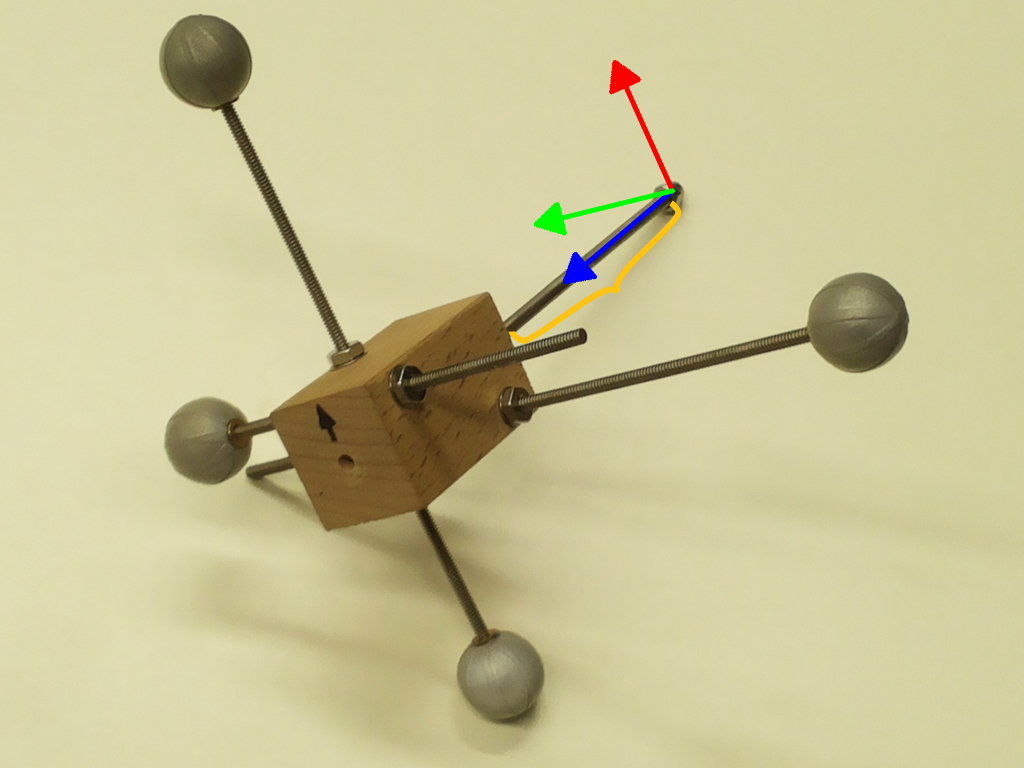
\includegraphics[width=0.45\textwidth]{fig/marker_set/marker_set_with_frame}
			\label{fig:MarkerSetEndEffectorWithFrame}
		}
		\subfigure[]{
			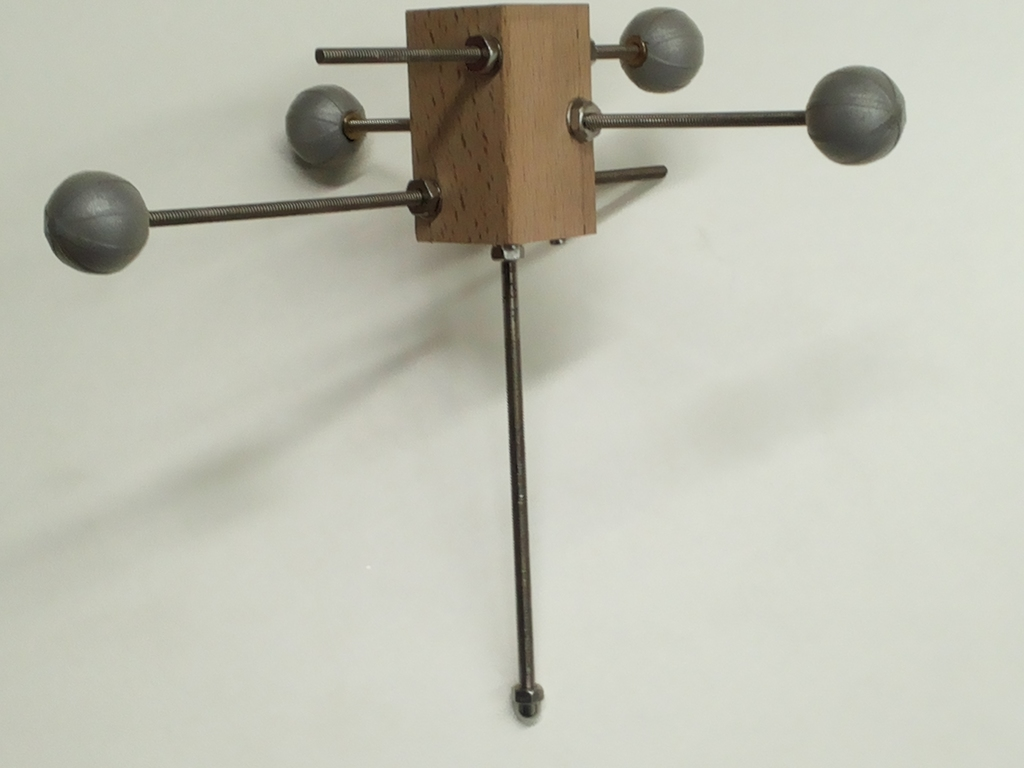
\includegraphics[width=0.45\textwidth]{fig/marker_set/marker_set_side}
			\label{fig:MarkerSetEndEffectorSide}
		}
		\caption{The marker set used in FBM3. The rod is marked by the yellow brace. The tip of the marker set is marked by the origin of the coordinate frame (the orientation of the coordinate frame is irrelevant here).}
		\label{fig:MarkerSetEndEffector}
	\end{center}
\end{figure}

\paragraph{Path specification}
The path to be executed by the robot is specified by:
\begin{itemize}
\item a mathematical description of a line in 2D space (see Figure~\ref{fig:FBM3_line_example} for an example):
    \begin{displaymath}
    f(x) = m \cdot x
    \end{displaymath}
    where
    \begin{itemize}
    \item $x$ is a distance in metres [$m$] along the x-axis of the robot-selected coordinate system
    \item $f(x)$ is a distance specified in metres [$m$] along the y-axis of the robot-selected coordinate system
    \item $m$ is the slope specified as a dimensionless scalar
    \end{itemize}
\item a mathematical description of a sine in 2D space (see Figure~\ref{fig:FBM3_sine_example} for an example):
    \begin{displaymath}
    f(x) = a \cdot \sin(c \cdot x)
    \end{displaymath}
    where
    \begin{itemize}
    \item $x$ is a distance in metres [$m$] along the x-axis of the robot-selected coordinate system
    \item $f(x)$ is a distance specified in metres [$m$] along the y-axis of the robot-selected coordinate system
    \item $a$ is the amplitude specified in metres [$m$]
    \item $c$ is a conversion from a distance to an angle specified in radians per metre [$\frac{rad}{m}$].
    \end{itemize}
\item distance between the calibration point and starting point specified in metres [$m$].
\item start of the path, specified in the domain of the mathematical description.
\item end of the path, specified in the domain of the mathematical description.
\item the concrete selection of the parameters for each benchmark will be announced before the competition.
\end{itemize}
\noindent
To exemplify the definition of start and end of the path assume a sine with $a = 0.1\;m$ and $c = 12.5\cdot\pi\;\frac{rad}{m}$. Let the start of the path be given as $start = 0\;m$ and the end of the path be given as $end = 0.2\;m$. Then the start point is $f(start = 0\;m) = 0\;m$ and the end point is $f(end = 0.2\;m) = 0.1 \;m$.

\begin{figure}[!htbp]
	\begin{center}
		\frame{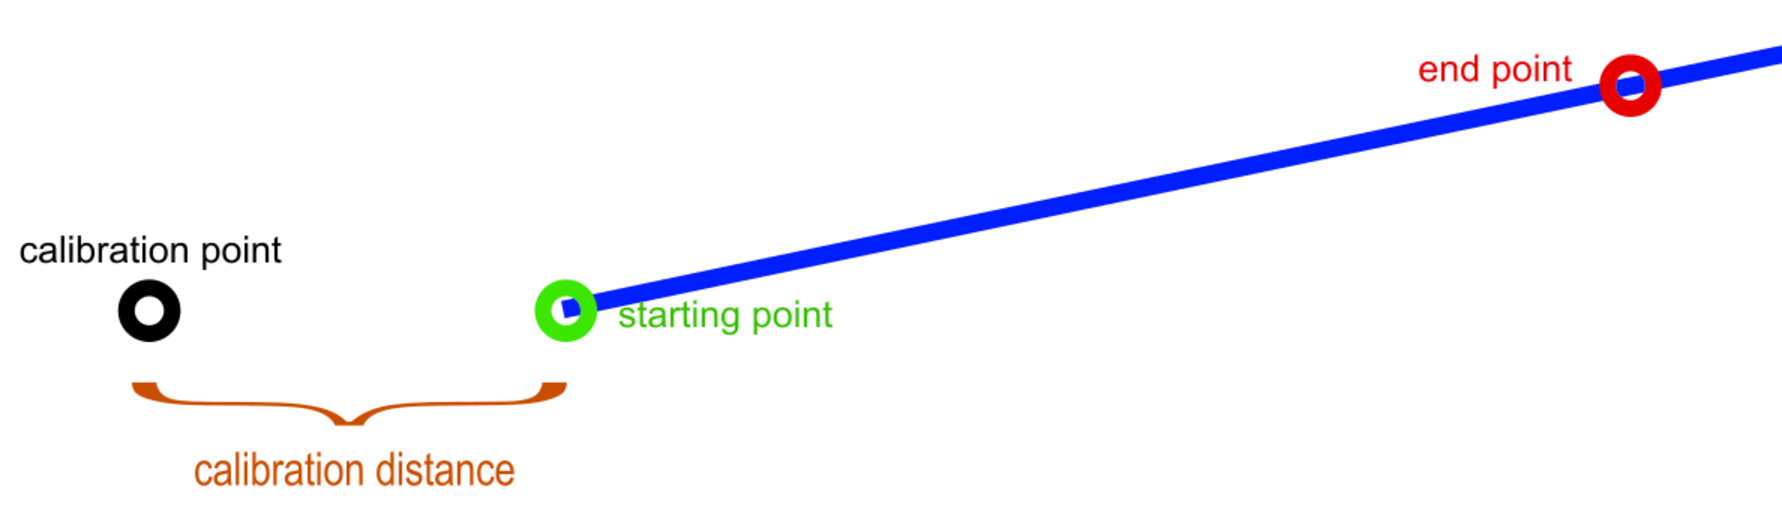
\includegraphics[scale=0.5,angle=0]{fig/FBM/atwork/fbm3/fbm3_line_example.pdf}}
		\caption{Example of a path on a straight line.}
		\label{fig:FBM3_line_example}
	\end{center}
\end{figure}

\begin{figure}[!htbp]
	\begin{center}
		\frame{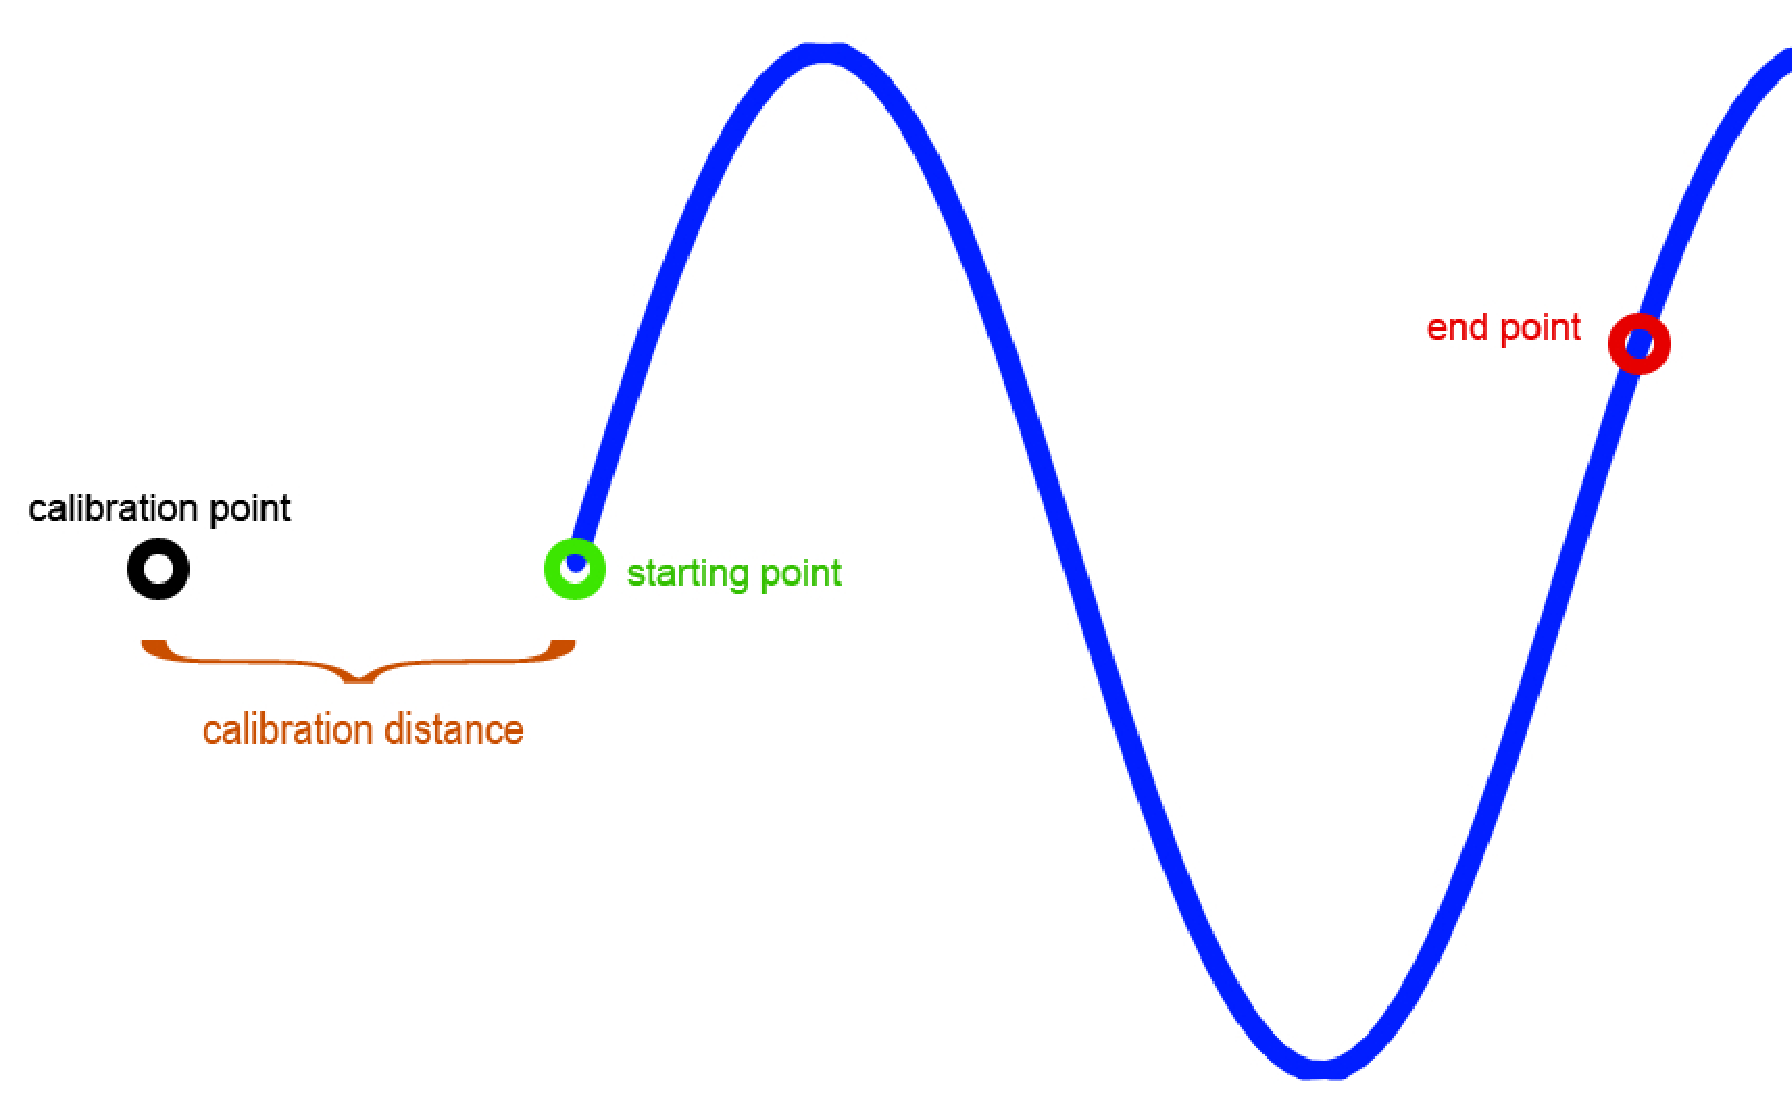
\includegraphics[scale=0.4,angle=0]{fig/FBM/atwork/fbm3/fbm3_sine_example.pdf}}
		\caption{Example of a path on a sine.}
		\label{fig:FBM3_sine_example}
	\end{center}
\end{figure}

\begin{figure}[!htbp]
	\begin{center}
		\frame{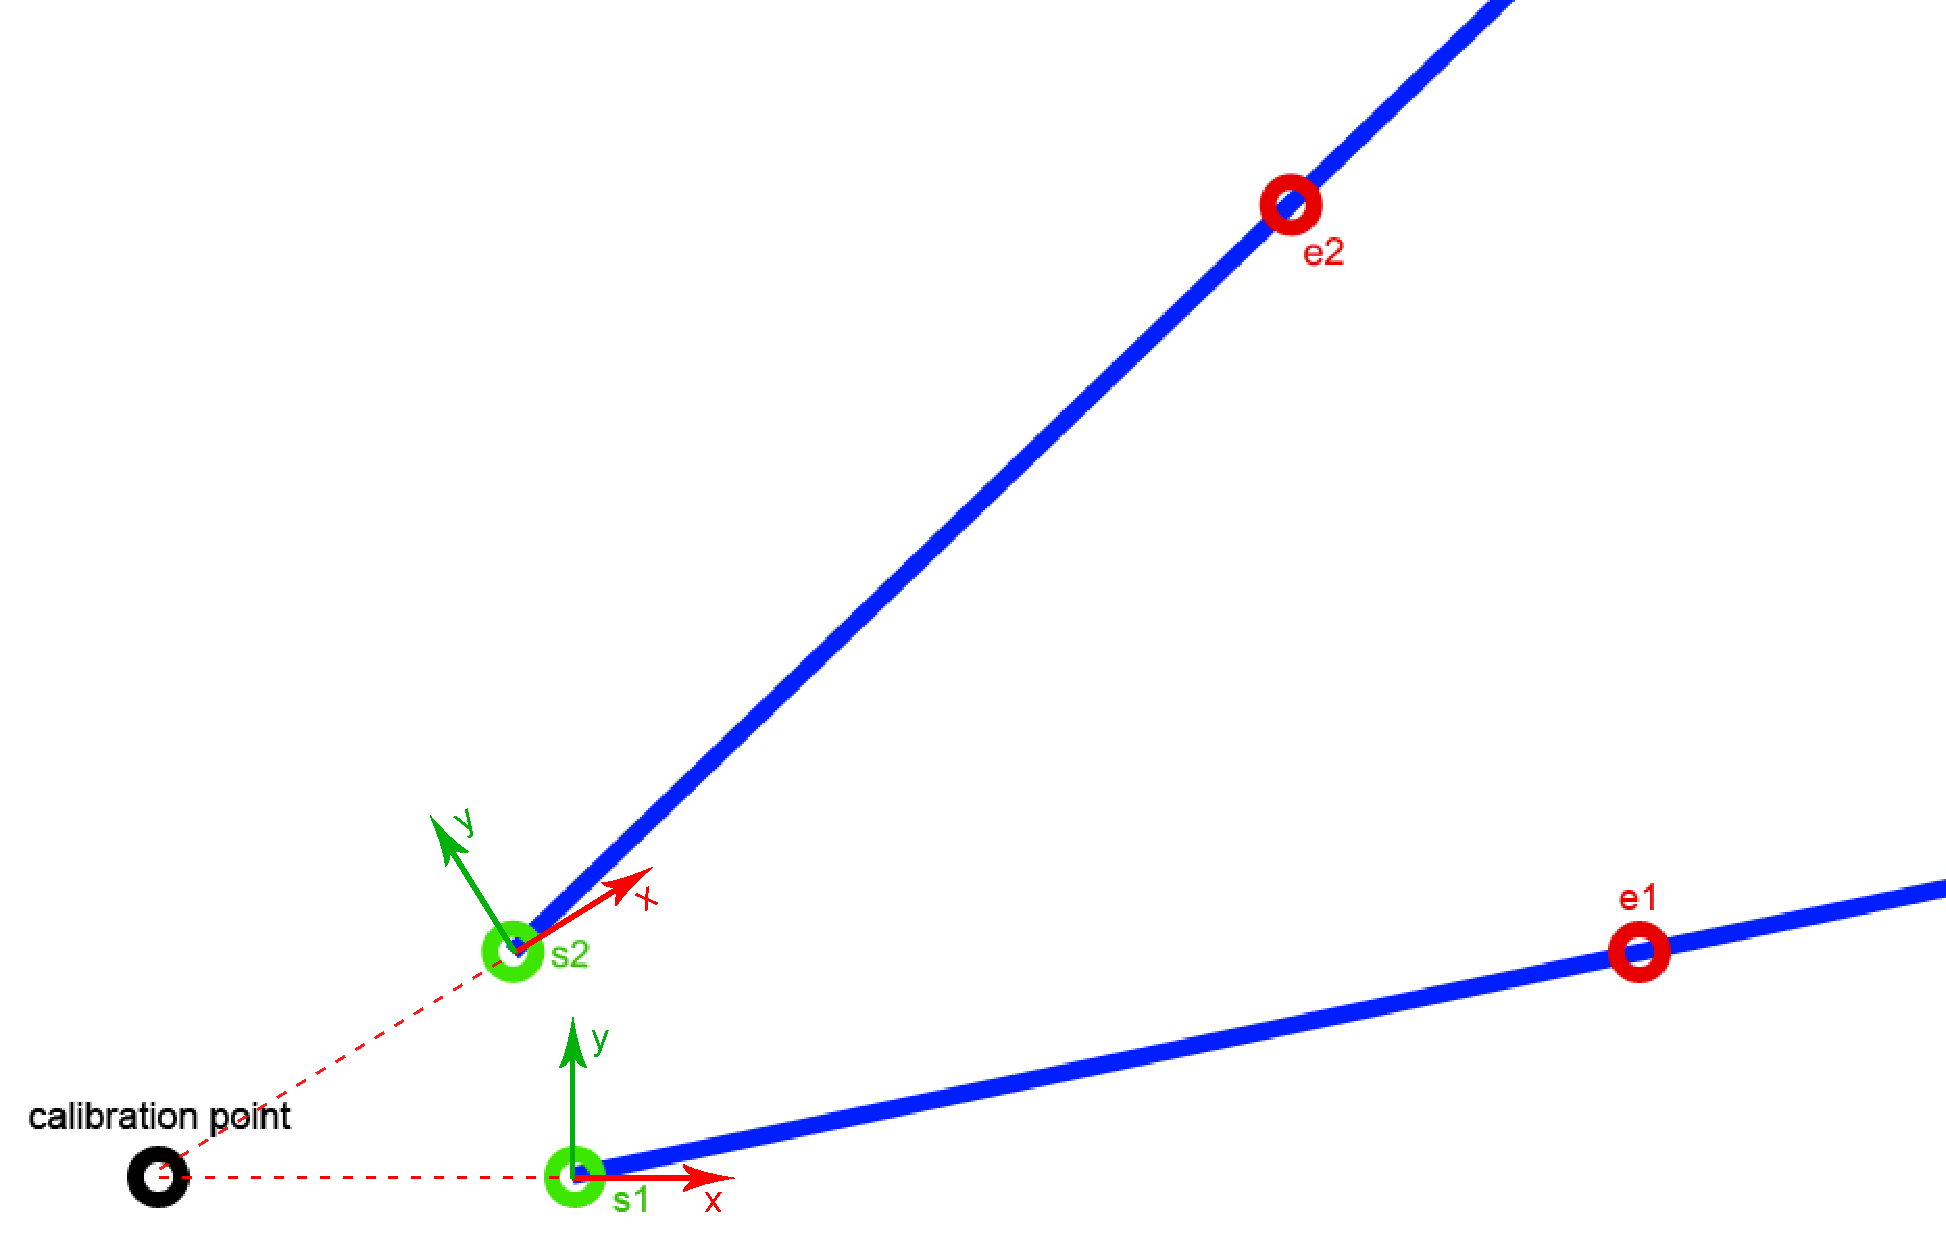
\includegraphics[scale=0.4,angle=0]{fig/FBM/atwork/fbm3/fbm3_rotation_example.pdf}}
		\caption{Example of two different starting points, $s1$ and $s2$. Note that the orientation of the path depends on the starting point.}
		\label{fig:FBM3_rotation_example}
	\end{center}
\end{figure}

%--------------------------------------------------------------------
\subsubsection{Expected Robot Behaviour or Output}
\label{sssec:ControlOutput}

The robot is placed in front of the test area (a planar surface). The robot is required to execute the provided path in a plane above the test area that is parallel to the ground, where the height above the ground is selected by the robot. Because the robot is free to select the reference frame w.r.t. which the path is executed, it must synchronize its internal reference frame with the benchmarking system's reference frame. This is achieved by a two-step calibration procedure as described below.

Each benchmark run consists of three different phases, namely \emph{calibration}, \emph{preparation} and \emph{execution}. In the calibration phase the robot moves the tip of the marker set to an arbitrary point on top of the test area which will be used as the \emph{calibration point}. Afterwards, in the preparation phase, the robot must move the tip of the marker set by the predefined \emph{calibration distance} (see Figure \ref{fig:FBM3_line_example} and Figure \ref{fig:FBM3_sine_example}) in a self-selected direction. The position reached after that motion is defined as the \emph{starting point} of the path. Finally, in the execution phase, the robot follows the path until the end point is reached or the time runs out. After each phase, the robot notifies the CFH that it has completed the phase.

The robot-selected coordinate system is derived based on the calibration procedure in the following way:
\begin{enumerate}
	\item The \emph{x-axis} is defined as the vector from the calibration point to the starting point.
	\item The \emph{z-axis} points upwards from the test area.
	\item The \emph{y-axis} complements the right-handed coordinate system.
\end{enumerate}
Figure~\ref{fig:FBM3_rotation_example} depicts two examples of such robot-selected coordinate systems.

Notice: this task is NOT executed with a feedback from any vision sensor from the team, but only testing a pre-planned path and the online continuous path control ability of the robot!

%--------------------------------------------------------------------
\subsubsection{Procedures and Rules}
\label{sssec:ControlProcedures}

Maximum time allowed for one functionality run is 4 minutes (60 seconds for calibration, 60 seconds for preparation and 120 seconds for execution). A run consists of (1) a calibration phase where the robot moves the tip of the marker set to the calibration point; (2) a preparation phase in which the tip of the marker set travels the calibration distance and (3) an execution phase where the robot follows the path.

Note: The tip of the marker set must maintain the height of the calibration point throughout a complete run. Only the position of the marker set's tip is considered, but not the orientation of the marker set.

\begin{description}
\item[Step 1] The robot is provided with the selection of the specific path and calibration distance in advance.
\item[Step 2] The CFH tells the robot to start the calibration phase.
\item[Step 3] The robot moves the tip of the marker set to its preferred calibration point. The robot reports to the CFH that it has finished the calibration phase.
\item[Step 4] The referee manually adjusts a sheet of paper such that the calibration point on the sheet coincides with the projection of the marker set to the test area.
\item[Step 5] The CFH tells the robot to start the preparation phase.
\item[Step 6] The robot moves the tip of the marker set until the calibration distance has been traveled. The robot reports to the CFH that it has finished the preparation phase.
\item[Step 7] The referee rotates the sheet of paper (with the calibration point acting as the pivot) such that the starting point coincides with the projection of the marker set to the test area.
\item[Step 8] The CFH tells the robot to start the execution phase.
\item[Step 9] The robot follows the path with the tip of the marker set and stops at the end point of the path. The robot reports the termination of the execution phase to the CFH.
\end{description} 

%--------------------------------------------------------------------
\subsubsection{Communication with CFH}
\label{sssec:CommCFHControl}

For this task benchmark the robot does not have to control any networked device in the environment. Only the communication as described below is necessary:

\begin{description}
\item[Step 1] The robot sends a \textbf{BeaconSignal} message at least every second.
\item[Step 2] The robot waits for a \textbf{BenchmarkState} message. It starts the calibration procedure when the \emph{phase} field is equal to CALIBRATION and the \emph{state} field is equal to RUNNING.
\item[Step 3] As soon as the robot reaches the calibration position, it sends a message of type \textbf{BenchmarkFeedback} to the CFH with the \emph{phase\_to\_terminate} field set to CALIBRATION. The robot should do this until the \textbf{BenchmarkState}'s \emph{phase} and \emph{state} fields have changed.
\item[Step 4] The robot waits for a \textbf{BenchmarkState} message. It starts the preparation procedure when the \emph{phase} field is equal to PREPARATION and the \emph{state} field is equal to RUNNING.
\item[Step 5] As soon as the robot reaches the preparation position, it sends a message of type \textbf{BenchmarkFeedback} to the CFH with the \emph{phase\_to\_terminate} field set to PREPARATION. The robot should do this until the \textbf{BenchmarkState}'s \emph{phase} and \emph{state} fields have changed.
\item[Step 6] The robot waits for a \textbf{BenchmarkState} message. It starts the benchmark execution when the \emph{phase} field is equal to EXECUTION and the \emph{state} field is equal to RUNNING.
\item[Step 7] As soon as the robot reaches the goal position, it sends a message of type \textbf{BenchmarkFeedback} to the CFH with the \emph{phase\_to\_terminate} field set to EXECUTION. The robot should do this until the \textbf{BenchmarkState}'s \emph{phase} and \emph{state} fields have changed.
\item[Step 8] The robot continues with Step 2.
\item[Step 9] The functionality benchmark ends when the \textbf{BenchmarkState}'s \emph{phase} field is equal to EXECUTION  and the \emph{state} field is equal to FINISHED.
\end{description}
\noindent
The messages to be sent and to be received can be seen on the Github repository located at \cite{rockin:CFHMessages}.

%--------------------------------------------------------------------
\subsubsection{Acquisition of Benchmarking Data}
\label{sssec:ControlData}

General information on the acquisition of benchmarking data is described in Section \ref{sec:TbmAcquisitionOfData}. There the \textbf{offline} part of the benchmarking data can be found.

\paragraph{Online Data} No online benchmarking data has to be sent to the CFH during this task benchmark.

\paragraph{Offline data} 
The additional information described in the following table has to be logged:
\\
\begin{table}[h]
	\centering
	\begin{footnotesize}
		\begin{tabular}{|l|l|l|l|}
			\hline
			Topic				 					&	Type		&	Frame Id		&	Notes \\ \hline\hline
			/rockin/reference\_pose\tablefootnote{Pose of the gripper at the reference point.} & geometry\_msgs/PoseStamped & /base\_link & -- \\ \hline
			/rockin/starting\_pose\tablefootnote{Pose of the gripper at the starting point.} 	& geometry\_msgs/PoseStamped & /base\_link & When starting \\ \hline
			/rockin/ending\_pose\tablefootnote{Pose of the gripper at the end of the trajectory.} 	& geometry\_msgs/PoseStamped & /base\_link & When ending \\ \hline
			/rockin/gripper\_pose\tablefootnote{Pose of the gripper during the whole trajectory.} & geometry\_msgs/PoseStamped & /base\_link & 10 Hz \\ \hline
			/rockin/arm\_joints\tablefootnote{Joints data}	& geometry\_msgs/JointState & /base\_link & 10 Hz \\ \hline
		\end{tabular}
	\end{footnotesize}
\end{table}

%--------------------------------------------------------------------
\subsubsection{Scoring and Ranking}
\label{sssec:ControlScoring}

Evaluation of the performance of a robot according to this functionality benchmark is based on:

\begin{enumerate}
	\item Accuracy of following the given path with the tip of the marker
	\item Number of completely executed path movements (maximum 5);
	\item Execution time (if less than the maximum allowed for the benchmark).
\end{enumerate}

The accuracy is evaluated as follows. Given the recorded marker path executed by the robot $r(l)$, the actual ground truth path $t(l)$ and $l$ as a parameter in $[0:1]$ with
\begin{itemize}
	\item $r(l) = ( x_{r(l)}, y_{r(l)} )$ the parametric representation of the robot path
	\item $t(l) = ( x_{t(l)}, y_{t(l)} )$ the parametric representation of the target path
\end{itemize}

\noindent the accuracy is computed by

\begin{equation}
\frac{1}{N} * \sum\nolimits_{l \in L_{sampled}} d(r(l), t(l))
\end{equation}

\noindent where $L_{sampled}$ is a subset of $L_{gt}$ and $L_{gt}$ are the values of $l$ to which corresponds a measure of the robot's path from the ground truth system, $N = |L_{sampled}|$ and $d()$ is the Euclidean distance. A more detailed analysis of this measure is available in the \roaw Wiki \cite{rockin:wiki:2015}.\\

The scoring of teams is based on the accuracy with which the robot follows the given path. In case of ties the overall execution time will be taken into account.

%--------------------------------------------------------------------
% EOF
%--------------------------------------------------------------------

%!TEX root = ./ERL Industrial Robots.tex

%--------------------------------------------------------------------
%--------------------------------------------------------------------
\subsection{Exploration Functionality (Shared with RoboCup@Work)}
\label{ssec:Exploration}

%--------------------------------------------------------------------
% IST-ID
\subsubsection{Functionality Description}
\label{sssec:FooOMDescription}

This benchmark evaluates the robot exploration and navigation capability.

%--------------------------------------------------------------------
% IST-ID
\subsubsection{Feature Variation}
\label{sssec:FooOMVariation}

This benchmark has the following feature variation:
\begin{itemize}
  \item{Distinct starting points, waypoints, and goal positions.}
  \item{Different number of waypoints to reach the goal.}
  \item{Different number of obstacles blocking the path.}
  \item{Different arena setup}
\end{itemize}

%--------------------------------------------------------------------
% IST-ID
\subsubsection{Input Provided}
\label{sssec:FooOMInput}

The robot will receive the following information:
\begin{itemize}
  \item{The starting position.}
  \item{A single location the robot must visit.}
  \item{The landmark for identifying the location the robot has to visit (QR code or color coding)}
  %\item{The maximum time allowed for the robot to go from each waypoint to the next waypoint, without penalization.} 
\end{itemize}

%--------------------------------------------------------------------
% IST-ID
\subsubsection{Expected Robot Behavior or Output}
\label{sssec:FooOMOutput}

Teams are required to set their robot on a specific starting position (that will be given to the teams before each run). Then, the robot receives, through the CFH, the start signal, as well as a location name that it must reach. The robot must notify the CFH when it has reached the location. The evaluation of the navigation will take into account the following two points:
\begin{itemize}
  \item The time spent by the robot to locate the location. 
  \item The number of times that the robot hits each obstacle. If the robot hits the same obstacle more than once, it will count as multiple hits.
\end{itemize}

The functionality benchmark ends as soon as one of the following situations occurs:
\begin{itemize}
  \item The robot reaches the specified location.
  \item The time available for the functionality benchmark expires.
  \item The robot damages any of the obstacles.
  \item The robot pushes or continually touches an obstacle for more than 3 seconds.
  \item The robot forces its path through an obstacle.
\end{itemize}

%--------------------------------------------------------------------
% IST-ID
\subsubsection{Procedures and Rules}
\label{sssec:FooOMProcedures}
All teams are required to perform this functionality benchmark according to the steps mentioned below. The task must be performed exclusively in autonomous mode. No teleoperation is allowed. Teams will have up to ten minutes to complete the functionality benchmark. Two minutes to move the robot to the correct starting position plus eight minutes to do the benchmarking.

\begin{description}
  \item [Step 1] The team is required to start their robot on a pre-defined starting position. This starting position will be given to the teams before each run.
  \item [Step 2] When the procedure starts, the robot receives a the location it has to go.
  \item [Step 3] Robot explores the arena and when it reaches the desired location sends back a signal to the CFH. The robot must avoid hitting any obstacle it encounters in its path.
  \item [Step 3] The procedure stops when the robot notifies it has reached the goal position, when the time given to complete the test expires, or when the robot hard-hits an obstacle.
\end{description}


%The obstacles can be of three types: 
%\begin{itemize}
%  \item \textbf{Static and previously mapped}: Hardware already present in the house such as furniture, doors, walls, defined in \ref{sssec:NRObjects}. The teams should already have this obstacles mapped from set-up days. These items will not change during this functionality benchmark.
%  \item \textbf{Static}: Items Granny Annie left lying on the ground. The obstacles may be of different shapes and sizes, are not previously known by the teams, and may be different in between runs.
%  \item \textbf{Dynamic}: Granny Annie's visitors. People moving inside the house. Obviously, the movement people will do is unpredictable.
%\end{itemize}



%--------------------------------------------------------------------
% POLIMI
\subsubsection{Acquisition of Benchmarking Data}
\label{sssec:FooOMData}
This functionality benchmark will be fully automated (no human operation will be allowed) and, for that, the robot has to communicate with the CFH. It will receive the target location from the CFH and it must send back a signal, each time it reaches a waypoint.
\begin{table}[h]
\centering
\begin{footnotesize}
\begin{tabular}{|l|l|p{5cm}|}
\hline
 Topic	&	Type  	  &	Notes \\ \hline\hline
 /roaw\_cfh/goal & geometry\_msgs/Pose2D & List of waypoints, sent by the CFH to the robot, when starting the task. \\ \hline
 /roaw\_cfh/reached\_waypoint & roaw\_cfh\_comm\_ros/UInt8 & Message sent by the robot to the CFH, when reaching a point. It must include the number of the respective waypoint in the sequence (starting from zero). \\ \hline
\end{tabular}
\end{footnotesize}
\end{table}


%--------------------------------------------------------------------
% IST-ID + ROME + POLIMI
\subsubsection{Scoring and Ranking}
\label{sssec:FooOMScoring}

Evaluation of the performance of the robot(a.k.a scoring) in the benchmark is based on:
\begin{enumerate}
 \item Time taken by the robot to find the location.
\end{enumerate}
%--------------------------------------------------------------------
% EOF
%--------------------------------------------------------------------


%%!TEX root = ./ERL Industrial Robots.tex

%--------------------------------------------------------------------
%--------------------------------------------------------------------
%--------------------------------------------------------------------
\section{\erlir Organization}
\label{sec:RoawOrganization}

%--------------------------------------------------------------------
%--------------------------------------------------------------------
\subsection{\erlir Management}
\label{ssec:RoawManagement}

The management structure of \erlir has been divided into three committees, namely \emph{Executive Committee}, \emph{Technical Committee} and the \emph{Organization Committee}. 
Pedro Lima (acting as the overall Coordinator of the challenges execution, within his role as \erl coordinator) is acting as \textbf{Supra-Chair}.
The roles and responsibilities of those committees are described in the following paragraphs.

%--------------------------------------------------------------------
\subsubsection{\erlir Executive Committee}
\label{sssec:RoawEC}

The Executive Committee (EC) is represented by the coordinators of each \erlir partner related to the respective activity area. 
The committee is mainly responsible for the overall coordination of \erlir activities and especially for dissemination in the scientific community. 
%	
\begin{itemize}	\topsep-12pt\itemsep-2pt\parsep0pt
\item Pedro Lima (Instituto Superior T\'ecnico, Portugal)
\item Daniele Nardi (Sapienza Universit\`a di Roma, Italy)
\item Gerhard Kraetzschmar (Bonn-Rhein-Sieg University, Germany)
\item Rainer Bischoff (KUKA Roboter GmbH, Germany)
\item Matteo Matteucci (Politecnico di Milano, Italy)
\end{itemize}


%--------------------------------------------------------------------
\subsubsection{\erlir Technical Committee}
\label{sssec:RoawTC}

The Technical Committee (TC) is responsible for the rules of the league. Each member of the committee is involved in maintaining and improving the current rule set and in the adherence of these rules. Other responsibilities include the qualification of teams, handling general technical issues within the league, deciding about giving awards in case the number of participants is lower than the thresholds specified in Section~\ref{sec:AwardCategories}, as well as resolving any conflicts inside the league during an ongoing competition. The members of the committee are further responsible for maintaining the \erlir infrastructure. 

The Technical Committee currently consists of the following members:
%
\begin{itemize}	\topsep-12pt\itemsep-2pt\parsep0pt
\item Alberto Pretto (Sapienza Universit\`a di Roma, Italy)
\item Rhama Dwiputra (Bonn-Rhein-Sieg University, Germany)
\item Tim Friedrich (KUKA Roboter GmbH, Germany)
\item Matteo Matteucci (Politecnico di Milano, Italy)
\end{itemize}
%
This committee can include members of the Executive Committee.

%--------------------------------------------------------------------
\subsubsection{\erlir Organizing Committee}
\label{sssec:RoawOC}

The Organizing Committee (OC) is responsible for the actual implementation of the competition, i.e.~providing everything what is required to perform the various tests. 
Specifically, this means providing setting up the test arena(s), providing any kind of objects (e.g.~manipulation objects), scheduling the tests, assigning and instructing referees, recording and publishing (intermediate) competition results and any other kind of management and advertisement duties before, during and after the competition. 

The Organizing Committee currently consists of the following members:
%
\begin{itemize}	\topsep-12pt\itemsep-2pt\parsep0pt
\item \textbf{Chair:} Tim Friedrich (KUKA Roboter GmbH, Germany)
\item Francesco Amigoni (Politecnico di Milano, Italy)
\item Tiago Veiga (Instituto Superior T\'ecnico, Portugal)
\item Frederik Hegger (Bonn-Rhein-Sieg University, Germany)
\item Graham Buchanan (InnoCentive EMEA, U.K.)
\end{itemize}
%

%--------------------------------------------------------------------
%--------------------------------------------------------------------
\subsection{\erlir Infrastructure}
\label{ssec:RoawInfrastrcuture}

%--------------------------------------------------------------------
\subsubsection{\erlir Web Page}
\label{sssec:RoawWeb}

The official \erlir website can be reached at
%
\begin{flushleft}
	\hspace*{1cm}\url{http://erl.rocks/} 
\end{flushleft}
%
On this web page, teams can find introductory information about the league itself as well as relevant information about upcoming events, the most recent version of the rule book, videos and pictures of past competitions and links to further resources like the official mailing list or wiki. 


%--------------------------------------------------------------------
\subsubsection{\erlir Mailing List}
\label{sssec:RoawMailingList}

The official \erlir mailing list maintained by the league is as follows
%
\begin{flushleft}
	\hspace*{1cm}\url{laber} 
\end{flushleft}
%
Anyone can subscribe by using the following subscription page.
%
\begin{flushleft}
	\hspace*{1cm}\url{bla}\\ 
\end{flushleft}
%
Every subscriber is requested to register either with an email address which already encodes the real name or alternatively specify it in the provided field at the subscription page. In order to prevent the mailing list from spammers, this mailing list is moderated. 

The mailing list will be used for any kind of official announcement, e.g.~upcoming \erlir competitions, rule changes, registration deadlines or infrastructure changes. Teams are welcome to raise any kind of question regarding the league on this list.

\subsection{\erlir Competition Organization}
\label{ssec:CompOrg}

%--------------------------------------------------------------------
\subsubsection{Qualification and Registration}
\label{sssec:CompQualReg}

Participation in \erlir requires successfully passing a qualification procedure. This procedure is to ensure a well-organized competition event and the safety of participants.
Depending on constraints imposed by a particular site or the number of teams interested to participate, it may not be possible to admit all interested teams to the competition.

All teams that intend to participate at the competition have to perform the following steps (using the forms at the web site \url{http://erl.rocks/}):
%
\begin{enumerate}	\topsep-12pt\itemsep-2pt\parsep0pt
	\item Preregistration (deadline: 31 May 2015) -- optional
	\item Submission of qualification material (e.g.~team description paper and video; deadline: 31 August 2015) -- mandatory
	\item Final registration (between 9 and 30 September 2015) -- mandatory, and for qualified teams only
\end{enumerate} 

%--------------------------------------------------------------------
\paragraph{Preregistration}
\label{par:CompPreregistration}

A team must provide the following information during the preregistration process:
%
\begin{itemize}	\topsep-12pt\itemsep-2pt\parsep0pt
	\item Team name + Affiliation
	\item Team leader name
	\item Team leader email address
	\item Expected number of team members
	\item Whether the team plan to bring their own robot or not
	\item Middleware used for software development
\end{itemize}
%
This step can be considered as an \emph{Intention of Participation} declaration and serves as planning basis for the Organizing Committee.

%--------------------------------------------------------------------
\paragraph{Qualification}
\label{par:CompQualification}

The qualification process serves a dual purpose: It should allow the Technical Committee to assess the safety of the robots a team intents to bring to a competition, and it should allow to rank teams according to a set of evaluation criteria in order to select the most promising teams for a competition, if not all interested teams can be permitted. The TC will select the qualified teams according to the qualification material provided by the teams. 

The evaluation criteria will include:
%
\begin{itemize}	\topsep-12pt\itemsep-2pt\parsep0pt
  \item Team description paper
  \item Team web site
  \item Relevant scientific contribution/publications
  \item Professional quality of robot and software
  \item Novelty of approach
  \item Relevance to industrial service robotics
  \item Performance in other competitions
  \item Contribution to \erlir league (e.g.~by organization of events or provision and sharing of knowledge)
\end{itemize}
%
The Team Description Paper (TDP) is a central element of the qualification process and has to be provided by each team as part of the qualification process. 
The TDP should at least contain the following information in the author/title section of the paper:
%
\begin{itemize}	\topsep-12pt\itemsep-2pt\parsep0pt
  \item Name of the team (title)
  \item Team members (authors), including the team leader
  \item Link to the team web site
  \item Contact information
\end{itemize}
%
The body of the TDP should contain information on the following:
focus of research/research interests:
%
\begin{itemize}	\topsep-12pt\itemsep-2pt\parsep0pt
  \item Description of the hardware, including an image of the robot(s)
  \item Description of the software, especially the functional and software architectures
  \item Main involved research areas in the team work
  \item Innovative technology (if any)
  \item Reusability of the system or parts thereof
  \item Applicability and relevance to industrial robotics
\end{itemize}
%
The team description paper should cover in detail the technical and scientific approach, while the team web site should be designed for a broader audience. Both the web site and the TDP have to be written in English.

The length of the team description paper is limited to 6 pages and has to be to submitted in the IEEE Conference Proceedings format\footnote{\url{http://www.ieee.org/conferences_events/conferences/publishing/templates.html}}.


%--------------------------------------------------------------------
\paragraph{Registration}
\label{par:CompRegistration}

Only if a team has passed the qualification procedure successfully it is allowed to register officially for the competition and has to provide additional information e.g.~the exact number of team members.
Please be advised that this year, a team participating in TBM(s) for one of the Challenges (\roah or \roaw) must participate in all FBMs for that Challenge.
Further information about the registration procedure will be communicated through the mailing list of qualified teams.
The number of people to register per team may be unlimited, but during the competition the organizers will provide space only for 6 persons to work at tables in the team area. 
During the final registration, each team has to designate one member as team leader.  A change of the team leader must be communicated to the Organizing Committee. 

%--------------------------------------------------------------------
\subsubsection{Setup and Schedule}
\label{sssec:CompSetupSchedule}

\erlir competition will take place in the main science museum Pavilion of Knowledge and Portugal Pavilion of Lisboa, from 17-23 November 2015.
%26-30

17--18 November will be the assembly days, during which the arenas, team areas, power, audiovisual equipment and other infrastructure will be put in place.

19--20 November will be setup days, that the teams can use to unpack their robots, calibrate the robot systems, and get information about the test bed, important objects and other relevant details. The site will be closed to the public.

There will be three competition days: 21, 22 and 23 November. During those days, the competitions will occur following the procedures and rules described in the subsections of this document with the same title. The site will be accessible to the public during the actual competitions.

The award and closing ceremony will take place in the evening of the last day, 23 November 2015.

Several satellite events, with the participation of industry and academia stakeholders, will take place during the five days of the main event. These include talks by members of RoCKIn's Advisory Board, and the assessment of the Competition by the members of RoCKIn's Experts Board.


\noindent
\begin{description}
	\item[Schedule:] For the scheduling of particular stages, tests, and technical challenges of the competition the following applies:
	%
	\begin{itemize}
	  	\item The exact schedule of task-functionality tests will be announced one week before the actual competition by the OC on both the website and the mailing list of qualified teams.
	  	\item In order to avoid excess of "traffic" inside the testbed, an additional schedule only for test slots will be established on site by the OC.
	  	\item A set of test slots will be assigned to each team between the official test slots, where a team has exclusive access to the testbed without any other team/robot inside the arena.
	\end{itemize}
	\item[Setup:] For the arrival, setup, and preparation of teams participating in the competition, the following procedures apply: 
	%	
	\begin{itemize}
	  	\item A first draft of the rule book will be made public on June 30th 2015.
		\item Revisions will be possible and updated in the online versions of the document, based on suggestions of all relevant stakeholders (including pre-registered and registered teams) until July 31th 2015.
		\item The final version of the rule book will be made public, no later than eight weeks before the actual event, by the TC, including all the items referred as open in this document (e.g., some benchmarking and scoring items) and revisions resulting from the discussion referred in the previous item.
	  	\item The competition side will be divided into a competition arena and a team area.
	  	\item The competition arena consists of one or more testbeds (the arena) and is open for public.
	  	\item The arena must be kept clean and in a presentable condition all the time.
	  	\item The team area is a dedicated area only for team members, no public access here.
	  	\item Each team will be assigned to a designated area with tables and chairs (based on the number of team members), with power sockets, a shelf internet connection and a reasonable area to park their robot and other equipment.
	\end{itemize}  
\end{description}

%--------------------------------------------------------------------
\subsubsection{Competition Execution}
\label{sssec:CompExec}

\begin{itemize}
\item Referees will be determined by the OC out of the group of team leaders and TC members.
\item The referees ensure the correct execution of a benchmark, are in charge of keeping the time and counting the scores, being always helped by a TC or OC member.
\item In case of any dangerous situation the referees are allowed to immediately stop a benchmark and trigger the emergency stop functionality of the respective robot.
\item The official language for all kind of communication within the league is English (e.g.,~team leader meetings, announcements, schedule).
\item The order in which the teams have to perform a particular benchmark will be determined by a draw through the OC.
\item The order will be announced on the day \underline{before} the actual benchmark.
\item No team members or other persons are allowed to be in the arena during an official benchmark (only if the rule book explicitly allows/requires this).
\item Regular team leader meetings (every day) will be organized and announced by the TC/OC during the competition in order to discuss open issues for upcoming benchmarks.
\end{itemize}

%--------------------------------------------------------------------
\subsubsection{Measurements Recording}
\label{par:CompMeasurements}

Several variables of interest will be recorded by the EC, TC and OC during the actual benchmarks of the teams during the competition, while performing their \emph{task} and \emph{functionality benchmarks}. Some of these will be performed by \erlir equipment, though requiring the installation of markers on the team robots. Other logging will require the teams to accommodate, in their software, modules that respond to solicitations from test bed-installed software. 
Details on these procedures will be provided closer to the competition dates, but the teams must be ready to commit to such requirements as one of the key requirements to be selected for the \erlir competitions.
%--------------------------------------------------------------------
% EOF
%--------------------------------------------------------------------


%--------------------------------------------------------------------
% EOF
%--------------------------------------------------------------------
